\documentclass[final]{fhnwreport}       	%[mode] = draft or final
                                        	%{class} = fhnwreport, article, 
                                        	%          report, book, beamer, standalone
%%---Main Packages-----------------------------------------------------------------------
\usepackage[english, ngerman]{babel}	%Mul­tilin­gual sup­port for LaTeX
\usepackage[T1]{fontenc}				%Stan­dard pack­age for se­lect­ing font en­cod­ings
\usepackage[utf8]{inputenc}				%Ac­cept dif­fer­ent in­put en­cod­ings
\usepackage{lmodern}                    %The newer Font-Set
\usepackage{textcomp}					%LaTeX sup­port for the Text Com­pan­ion fonts
\usepackage{caption}					%Customising captions in floating environments
\usepackage{graphicx} 					%En­hanced sup­port for graph­ics
\usepackage{float}						%Im­proved in­ter­face for float­ing ob­jects
\usepackage{ifdraft}                    %Let you check if the doc is in draft mode
\usepackage{enumitem}


%%---Useful Packages---------------------------------------------------------------------
\usepackage{colortbl}	
\usepackage{color}						%Colour control for LaTeX documents
\usepackage[pdftex,dvipsnames,tabl]{xcolor}  %Driver-in­de­pen­dent color ex­ten­sions for LaTeX
\usepackage{csquotes}                   %Simpler quoting with \enquote{}
\usepackage{siunitx} 					%A com­pre­hen­sive (SI) units pack­age
%\usepackage{listings}					%Type­set source code list­ings us­ing LaTeX
\usepackage[bottom]{footmisc}			%A range of foot­note op­tions
\usepackage{footnote}					%Im­prove on LaTeX's foot­note han­dling
\usepackage{verbatim}					%Reim­ple­men­ta­tion of and ex­ten­sions to LaTeX ver­ba­tim
\usepackage[textsize=footnotesize]{todonotes} %Mark­ing things to do in a LaTeX doc­u­ment
\usepackage{titling}					%Control over the typesetting of the \maketitle command
\usepackage[euler]{textgreek}		%Allows to write greek letters without entering math-mode (\textOmega)

%%---Tikz Packages-----------------------------------------------------------------------
\usepackage{standalone}
\usepackage{tikz}
\usepackage{circuitikz}
\usetikzlibrary{arrows}
\usetikzlibrary{calc}
\usetikzlibrary{intersections}

%%---Math Packages-----------------------------------------------------------------------
\usepackage{amsmath}					%AMS math­e­mat­i­cal fa­cil­i­ties for LaTeX
\usepackage{amssymb}					%Type­set­ting symbols (AMS style)

%\usepackage{amstext}
%\usepackage{amsfonts}
%\usepackage{breqn}
%\usepackage{array}						%Ex­tend­ing the ar­ray and tab­u­lar en­vi­ron­ments
%\usepackage{amsthm}					%Type­set­ting the­o­rems (AMS style)

%%---Table Packages----------------------------------------------------------------------
\usepackage{tabularx}					%Tab­u­lars with ad­justable-width columns
%\usepackage{longtable}
%\usepackage{multirow}					%Create tab­u­lar cells span­ning mul­ti­ple rows
\usepackage{multicol}					%In­ter­mix sin­gle and mul­ti­ple columns



%%---PDF / Figure Packages---------------------------------------------------------------
\usepackage{pdfpages}					%In­clude PDF doc­u­ments in LaTeX
%\usepackage{pdflscape}					%Make land­scape pages dis­play as land­scape
%\usepackage{subfig}					    %Fig­ures di­vided into sub­fig­ures

%%---Other Packages----------------------------------------------------------------------
%\usepackage{xargs}                     %De­fine com­mands with many op­tional ar­gu­ments


%%---Bibliography------------------------------------------------------------------------
\usepackage[style=ieee,urldate=comp,backend=biber]{biblatex}
\addbibresource{literature/bibliography.bib}

%%---Main Settings-----------------------------------------------------------------------
\graphicspath{{./graphics/}}			%Defines the graphicspath
\geometry{twoside=false}				    %twoside=false disables the "bookstyle"
\setlength{\marginparwidth}{2cm}
\overfullrule=5em						%Creates a black rule if text goes over the margins => debugging




%%---User Definitions--------------------------------------------------------------------
%%Tabel-Definitions: (requires \usepackage{tabularx})
\newcolumntype{L}[1]{>{\raggedright\arraybackslash}p{#1}}    %column-width and alignment
\newcolumntype{C}[1]{>{\centering\arraybackslash}p{#1}}
\newcolumntype{R}[1]{>{\raggedleft\arraybackslash}p{#1}}
\usepackage{subcaption}


%%---Optional Package Settings-----------------------------------------------------------
%Listings-Settings: (requires \usepackage{listings}) => Example with Matlab Code
%\lstset{language=Matlab,%
%    basicstyle=\footnotesize\ttfamily,
%    breaklines=false,%
%    morekeywords={switch, case, otherwise},
 %   keywordstyle=\color{Blue},%
 %  tabsize=2,
    %morekeywords=[2]{1}, keywordstyle=[2]{\color{black}},
%    identifierstyle=\color{Black},%
%    stringstyle=\color{Purple},
%    commentstyle=\color{Green},%
%    showstringspaces=false,%without this there will be a symbol in the places where there is a space
%    numbers=left,%
%    numberstyle={\tiny \color{black}},% size of the numbers
%    numbersep=9pt, % this defines how far the numbers are from the text
    %emph=[1]{word1, word2,...},emphstyle=[1]\color{red}
%}							

%Hurenkinder und Schusterjungen verhindern (kein Scherz, Google es)
\clubpenalty10000
\widowpenalty10000
\displaywidowpenalty=10000	



%Titel mit Mathematik immer fett drucken
\usepackage{sectsty}
\allsectionsfont{\boldmath}



			               	%loads all packages, definitions and settings											
\title{Fachbericht}  		        		%Project Title
\author{Team Schenk \& Aebi}      				    %Document Type => Technical Report, ...
\date{\today}          				   	%Place and Date

\begin{document}

%%---TITLEPAGE---------------------------------------------------------------------------------
\thispagestyle{empty}
%	\ohead{\includegraphics[scale=0.5]{Bilder/Logo_FHNW.jpg}}
	\begin{figure}
		 \vspace*{-\topskip}\vspace*{-\headsep}
		
\includegraphics[scale=1]{graphics/fhnw_ht_logo_de.pdf}
	\end{figure}
	\begin{center}
		\vspace*{2cm}
		{\huge{\textbf{\thetitle}}}\\
		\vspace*{0.5cm}
		
		{\scshape\Large Projekt 6 Cocktailmaschine - \theauthor \\} \Large{\today}
		\vfill
		\begin{normalsize}
			{\begin{tabbing}
					\textbf{Betreuender Dozent:} \hspace{5cm}\= Prof. Dr. Schleuniger, Pascal\\[0.8cm]		
					\textbf{Team:} \>Schenk, Kim \\ \>Aebi, Robin\\[0.8cm]
					\textbf{Studiengang:} \>Elektro- und Informationstechnik
					\\[0.8cm]	\textbf{Semester:} \>Frühlingssemester 2020
			\end{tabbing}}
		\end{normalsize}
		\vfill
	\end{center}
\clearpage
			
%%---ABSTRACT----------------------------------------------------------------------------
\selectlanguage{english}				%ngerman or english
\thispagestyle{empty}
\paragraph{Danksagung}\mbox{}

Da diese Arbeit zur Zeit des Corona bedingten Lockdowns entstanden ist und keine Möglichkeit bestand in den Schulwerkstätten zu arbeiten, konnte nicht auf externe Hilfe verzichtet werden. Vor allem auch weil die Arbeit ein voll umfängliches Produkt darstellt, welches nicht nur elektrotechnische sondern auch mechanische Komponenten beinhaltet wurde eine gesamte Werkstatt benötigt. Diese wurde und von Claudia und Thomas Aebi zur Verfügung gestellt. Weiter wurden einige mechanische Komponenten auf der Drehbank angefertigt, was spezielles Equipment voraus setzte. Dabei wurden wir von Peter Aebi fachkräftig unterstützt. Im weiteren konnten wir uns jeder Zeit auf Herrn Christoph Biel verlassen, welcher die Studenten mit viel Herzblut jeder Zeit unterstützt. Sei es wenn man Messgeräte benötigt, Bestellungen erfassen oder Geld zurückfordern muss. Zu guter Letzt wurden wir durch das ganze Projekt hindurch von unserem Fachcoach Herrn Schleuniger unterstützt. Bei all diesen Personen wollen wir uns herzlichst bedanken. Ohne diese Mithilfe wäre es uns nicht möglich gewesen dieses Projekt auf diese Weise zu vollenden.     

\newpage




\begin{abstract}

Der technologische Fortschritt ist seit Jahren am explodieren. Das Internet der Dinge, oder auf Englisch auch Internet of things, kurz IoT, ist ein Produkt aus diesem Fortschritt. Es beschreibt ein Netz aus physikalischen und virtuellen Komponenten, welche miteinander kommunizieren, um einem Grösseren ganzen zu dienen. Im Zentrum steht nebst der Interaktion zwischen Mensch und elektronischen Systemen die Interaktion zwischen verschiedenen Systemen. In dieser Bachelorthesis wird anhand der Entwicklung einer IoT-Cocktailmaschine demonstriert, welche Teilsysteme wie genutzt werden können, um ein fertiges Produkt zu entwickeln.
Die Herausforderung liegt im gesamten Produktentwicklungsprozess und umfasst:\\

\begin{itemize}
\item die Projektauswahl, -Planung und -Abgrenzung
\item das Erstellen der Anforderungen an das Gesamtsystem und der darin enthaltenen Teilsysteme
\item die Wahl, das Testen, Implementieren der Komponenten
\item die Evaluation des Gesamtsystems
\end{itemize}
\mbox{}\\

Für die Umsetzung benötigt es einen Software- , einen elektronischen und einen mechanischen Teil.
Der mechanische Teil beinhaltet die Unterbringung der Zutaten und der Elektronik, der Beförderung und Messung der Flüssigkeiten mittels Pumpen und Durchflusssensoren sowie die Bewegung des Glases mit einem bürstenlosen Gleichstrommotor. Die Verschalung rundet die Maschine ab und verhindert, dass sensible Teile angefasst oder nass werden können.
Zum elektrotechnischen Teil gehört unter anderem ein Display, über welches der Benutzer die Cocktails auswählen, erstellen oder bearbeiten kann. Eine mikroSD-Karte ermöglicht Cocktails, Zutaten und maschinenspezifische Zustände zu speichern. Ein RFID-Reader liest Tags aus, was es ermöglicht Lieblingsgetränke zu hinterlegen und direkt in der Maschine anzuwählen.
Für die Verbindung zwischen Android-Applikation und Cocktailmaschine wird ein Wireless-/Bluetoothmodul verwendet. Mittels MOSFET-Schaltungen werden während der Erstellung von Cocktails die Pumpen vom Mikrocontroller ein- und ausgeschaltet. Die Ansteuerung und Regelung des bürstenlosen Gleichstrommotors ergibt sich aus einem FOC-Treiber und einem Gate-Treiber. Der ABN-Encoder liefert das Feedback zur Lage des Rotors, welches benötigt wird als Regelparameter für den FOC-Treiber.
Die entwickelte Leiterplatine gehört zum Elektronikteil und bildet das Bindeglied zwischen Mechanik und Elektronik.
Der Softwareteil wird in vier Teilsoftwares geteilt. Alle Teile werden in verschiedenen Sprachen geschrieben. Die Firmware auf dem Mikrocontroller, welche in C geschrieben wurde, regelt den Programmfluss der gesamten Maschine. Die Firmware auf dem Wireless-/Bluetoothmodul, welche in Arduino geschrieben wurde, bildet die Schnittstelle zwischen den Signalen der Android-Applikation und der Firmware. Die Android-Applikation wurde mit dem Online-Tool App-Inventor entwickelt und ermöglicht dem Anwender Cocktails über Fernzugriff zu erstellen und einem RFID-Tag zu zu weisen. Bei der letzten Programmierumgebung handelt es scih um den Nextion Editor, mit welchem Nextion Displays Programmiert werden können.


Damit alle Komponenten ansteuerbar sind, mussten einige Anpassungen an der Hardware vorgenommen werden. Dazu gehören aufgrund von Störungen auf dem SPI-Bus das Umlegen der SPI-Leitungen des RFID-Readers vom Mikrocontroller auf das Wireless-/Bluetoothmodul und das Umlegen der SPI-Leitungen des FOC-Treibers auf ein separates Software-SPI. Die Motorengruppe läuft aufgrund von Defekten auf der Leiterplatine mit externen Boards. Die Firmware läuft bis auf wenige Punkte sauber. Dazu gehört zum Beispiel, dass der Abbruchprozess beim Erstellen eines Getränkes nicht wunschgemäss Funktioniert. Die gesetzten Ziele wurden alle erreicht werden. Ausserdem wurden fast alle Pflichtziele erfüllt.





%Die in dieser Bachelorthesis entwickelte Cocktailmaschine ist ein IoT\footnote{\textbf{I}nternet \textbf{o}f \textbf{T}hings}-Produkt. Die Elemente sind eingebettet in Sensoren, Software und andere Technologien, welche es erlauben mit anderen Geräten zu kommunizieren. Zu den Elementen gehören ein Mikrocontroller mit zugehöriger Programmierschnittstelle, zwölf Pumpen sowie zugehörige Durchflusssensoren, ein RFID-Transponder, ein WiFi/Bluetooth-Modul mit zugehöriger Programmierschnittstelle, eine SD-Karte, ein FOC-Motorentreiber mit zugehörigem Kraft-Teil, ein Display und eine RGBW-LED-Regelung. Anhand der ersten Erfahrungen im Projekt 5 wurde eine Leiterplatine gelayoutet, welche die erwähnten Elemente verbindet. Über eine Android-Applikation wird den Benutzern die Möglichkeit geboten, einen neuen Cocktail zu erstellen oder das Lieblingsgetränk auszuwählen. Das gewählte Getränk kann dann vor Ort über den RFID-Tag bestellt werden. Die Mechanik besteht aus einem Aluminiumgerüst, welches verschalt wurde. Zusätzlich wurde zur Kühlhaltung eine Styroporbox um die Zutaten gebaut. Ein durch einen Motor angetriebener Schlitten fährt das Glas unter den gewünschten Flüssigkeitsauslass, wo das Glas befüllt wird. Die Dokumentation enthält eine Beschreibung der Platine und der darauf befindenden Elementen, eine Anleitung zur Inbetriebnahme der Elemente und einen Software-Teil. Das Produkt wurde physikalisch abgegeben und ist voll funktionsfähig.

\end{abstract}


%%---TABLE OF CONTENTS-------------------------------------------------------------------
\pagenumbering{Roman}		
\selectlanguage{ngerman}				%ngerman or english
\setcounter{tocdepth}{2}
\tableofcontents
\clearpage

%%---TEXT--------------------------------------------------------------------------------
\pagenumbering{arabic}
\clearpage
\section{Einleitung}
\label{sec:Einleitung}

Eine gelungene Party auf die Beine zu stellen verlangt einem einiges ab. Vor allem kostet es eine Menge Aufwand und Zeit. Dies gilt besonders, wenn es darum geht mit vielen Freunden zusammen zu feiern. Neben der gelungenen Musikauswahl und den Snacks darf eines auf gar keinen Fall fehlen, die Getränke. Um diese sicherzustellen, gibt es mehrere Möglichkeiten. Einerseits könnte jeder seine eigenen Getränke mitbringen, was jedoch bedeutet, dass es unter Umständen eine riesige Sauerei gibt oder viele Flaschen in der Gegend rumstehen. Anderseits könnte man als Gastgeber selber anbieten Cocktails zu mixen und so den Getränkenachschub zu gewährleisten. Da gibt es jedoch ein grosses Problem. Denn wären wir die Gastgeber, so würden wir nicht den ganzen Abend hinter der Bar stehen wollen, sondern lieber bedenkenlos mitfeiern. Damit genau dies möglich ist haben wir uns in diesem und dem nächsten Projekt (5\&6) dazu entschieden eine automatisierte Cocktailmaschine zu entwerfen. Diese soll vollkommen autonom arbeiten und sollte problemlos von jeder beliebigen Person und in fast jedem Zustand bedient werden können. 

In den folgenden Kapiteln ist dokumentiert, wie die Cocktailmaschine aussehen soll und aus welchen Teilsystemen diese bestehen wird. Ausserdem werden die einzelnen Teilsysteme genauer unter die Lupe genommen und in einem systemspezifischen Testverfahren evaluiert. Dieses Projekt bietet demnach die Basis des Projekt 6 und soll dieses so gut wie möglich vorbereiten.

\pagebreak
\section{Ausgangslage}
\label{sec:Ausgangslage}

Die Basis für das Projekt 6 hat das Projekt 5 gebildet, in welchem ein Konzept erstellt wurde, welches die Hauptkomponenten der Maschine festlegte und deren Arbeitsweise. Aus dieser Entscheidungsfindung wurde dann ein Blockschaltbild erstellt, welches in Abbildung \ref{fig:P5_Blockschaltbild_Partymixer} zu sehen ist. Ein weiterer Teil des Projekt 5 war es, die gewählten Komponenten und die daraus entstandenen Teilsysteme in einem Testaufbau aufzubauen und zu evaluieren. Dazu gehörten die Speisungen (48V, 12V, 5V und 3.3V), der Mikrocontroller, das Display, der Motor, die Pumpenansteuerung und die Durchflussmessgeräte.

\begin{figure}[H]
\center
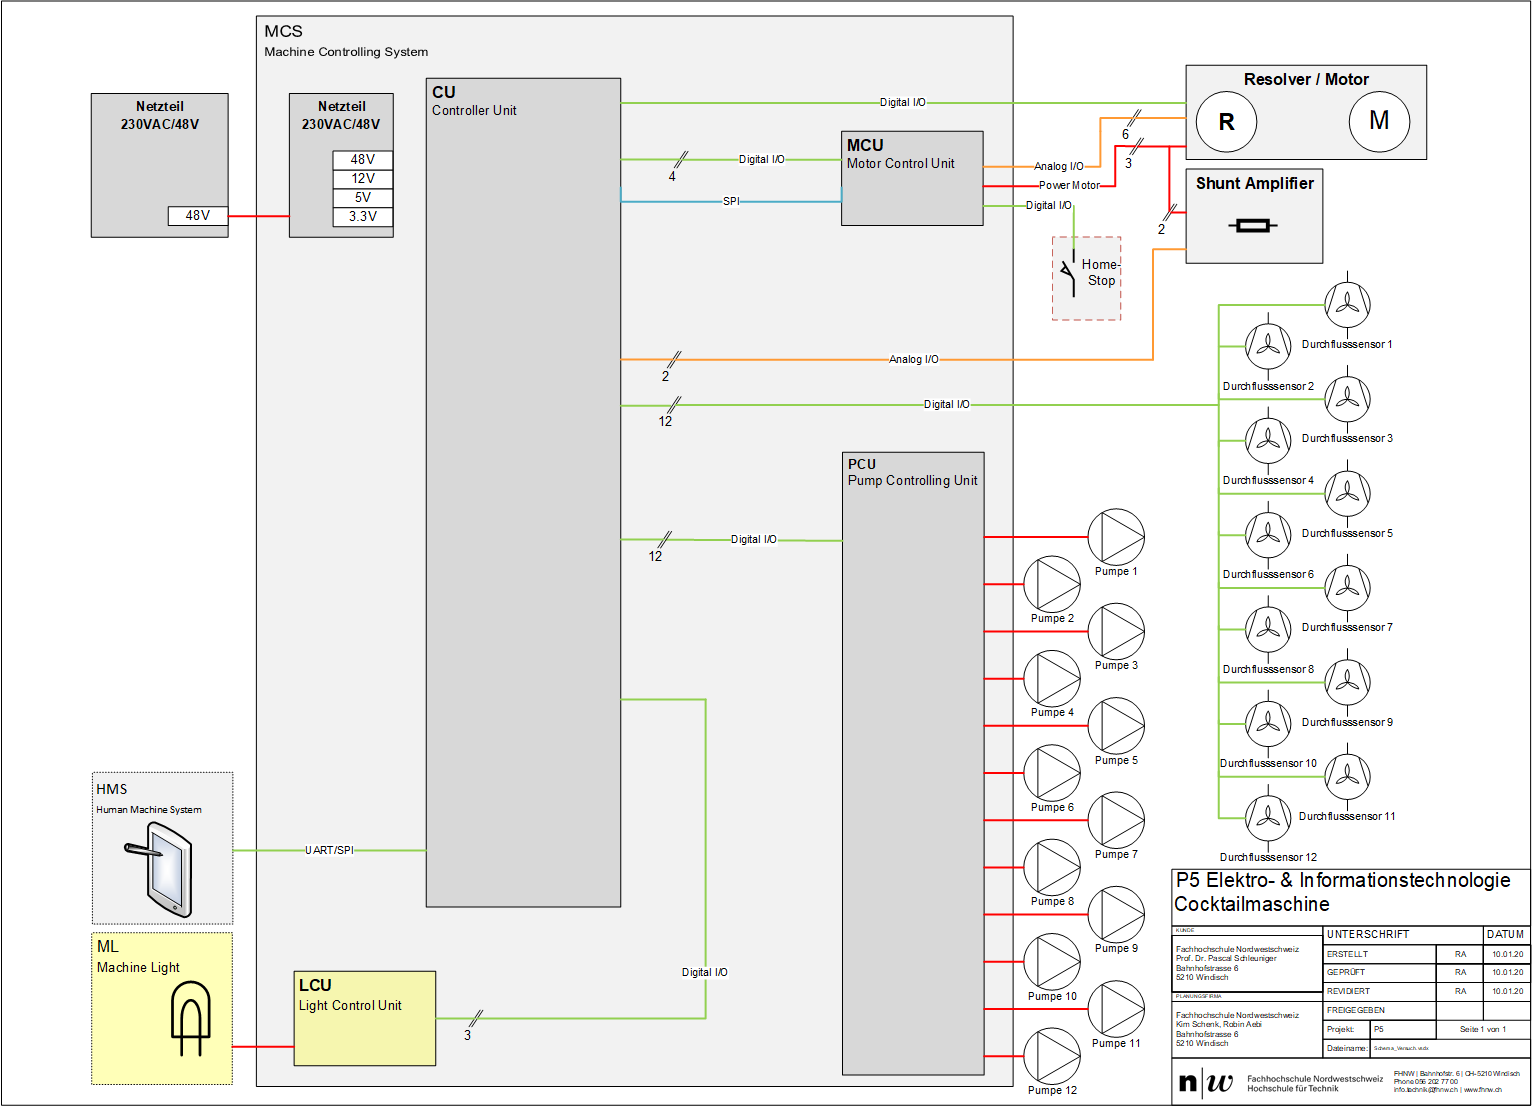
\includegraphics[angle=90, width = 0.82\textwidth]{graphics/P5-Blockschema}
\caption{Blockschaltbild des PartyMixer's gemäss Projekt 5.}
\label{fig:P5_Blockschaltbild_Partymixer}
\end{figure}

\newpage



\subsection{Blockschaltbild}
\label{subsec:Blockschaldbild}



%\subsection{Komponentenauswahl}
\label{subsec:Komponentenauswahl}

Um die Anforderungen gemäss Blockschaltbild erfüllen zu können sind neue Komponenten implementiert worden. Diese sollen nun genauer unter die Lupe genommen werden.

Speisungen: 
\begin{itemize}
\item Sorgen für die notwendigen Betriebsspannungen
\end{itemize}

Mikrocontroller: 
\begin{itemize}
\item Sorgen für die notwendigen Betriebsspannungen
\end{itemize}



\newpage

\section{Neue Hardware}
\label{sec:Neue Hardware}

Im folgenden Kapitel werden die Hardware-Teile beschrieben, welche im Projekt 5 noch nicht erarbeitet wurden. Zuerst werden grundlegende Anforderungen und Inhalte beschrieben, welche zur Auswahl der Bauteile feführt hat.

\subsection{Wirelessmodul}
\label{subsec:Wirelessmodul}

Über einen Web-Host soll der User die Möglickeit haben, Getränke auszuwähen und seinem RFID-Chip zuzuordnen, sowie diverse kleinere Einstellungen an der Maschine vorzunemen. Dazu wird ein WiFi-Modul benötigt.

Aufgrund schon bestehender Erfahrungen wurde ein Espressif ESP-Modul ausgewählt. Grundsätzlich standen zwei Modelle zur Auswahl. Das ESP8266 und das ESP32. Für die Cocktailmaschine wurde das ESP32 ausgewählt, da dies einfach Leistungsstärker ist. Die genauen Datenvergleiche sind in Tabelle \ref{tab:ESP} ersichtlich.

\begin{table}[!h]
\begin{tabularx}{\textwidth}{l|X|X}
MCU                    & Xtensa Single-core 32-bit L106 & Xtensa Dual-Core 32-bit LX6 \\ \hline
802.11 b/g/n     		& HT20                           & HT40                                       \\
Bluetooth              	& No                             & Bluetooth 4.2 and BLE                      \\
Arbeitsfrequenz			& 80 MHz                         & 160 MHz                                    \\
SRAM                   	& No                             & Yes                                         \\
Flash                  	& No                             & Yes                                          \\
GPIO                   	& 17                             & 36                                         \\
SPI/I2C/I2S/UART       	& 2/1/2/2                        & 4/2/2/2                                    \\
ADC                    	& 10-bit                         & 12-bit                                     \\
Ethernet Interface 		& No                             & Yes                                          \\
Touchsensor           	& No                             & Yes                                          \\
Temperatursensor     	& No                             & Yes                                          \\
Hall-Sensor     		& No                             & Yes \\
Arbeitstemperatur    	& -40ºC to 125ºC                 & -40ºC to 125ºC                             \\
Price                  	& \$ (3\$ - \$6)                   & \$\$ (\$6 - \$12)                             
\end{tabularx}
\caption{Vergleich ESP8266 zu ESP32.}
\label{tab:ESP}
\end{table}

Wichtig ist, dass ein ESP ausgewählt wird, welches einen Anschluss für eine abgesetzte Antenne hat, da die Leiterplatte im Gehäuse verbaut wird. Dazu eignet sich der Espressif ESP32-32U. Dieser ist in Abbildung \ref{fig:Produktbild_ESP32_32U_Wroom} als Wroom dargestellt und in Abbildung \ref{fig:Produktbild_ESP32_32U_DevKit} als Development Kit.

\begin{figure}[!h]
\center
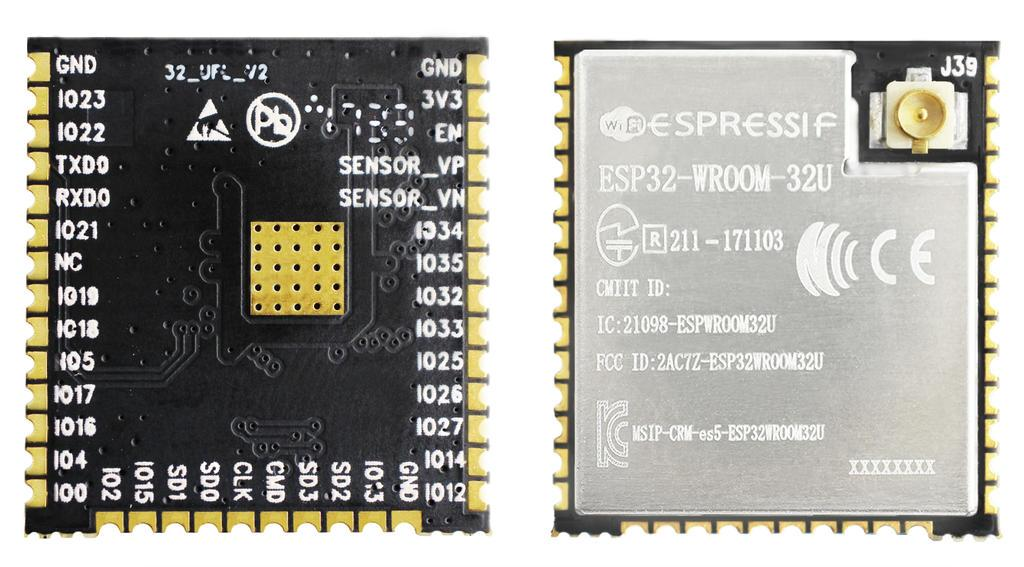
\includegraphics[width = 0.4\textwidth]{graphics/Produktbild_ESP32}
\caption{ESP32-32U Wroom.}
\label{fig:Produktbild_USB_UART_ESP}
\end{figure}

\begin{figure}[!h]
\center
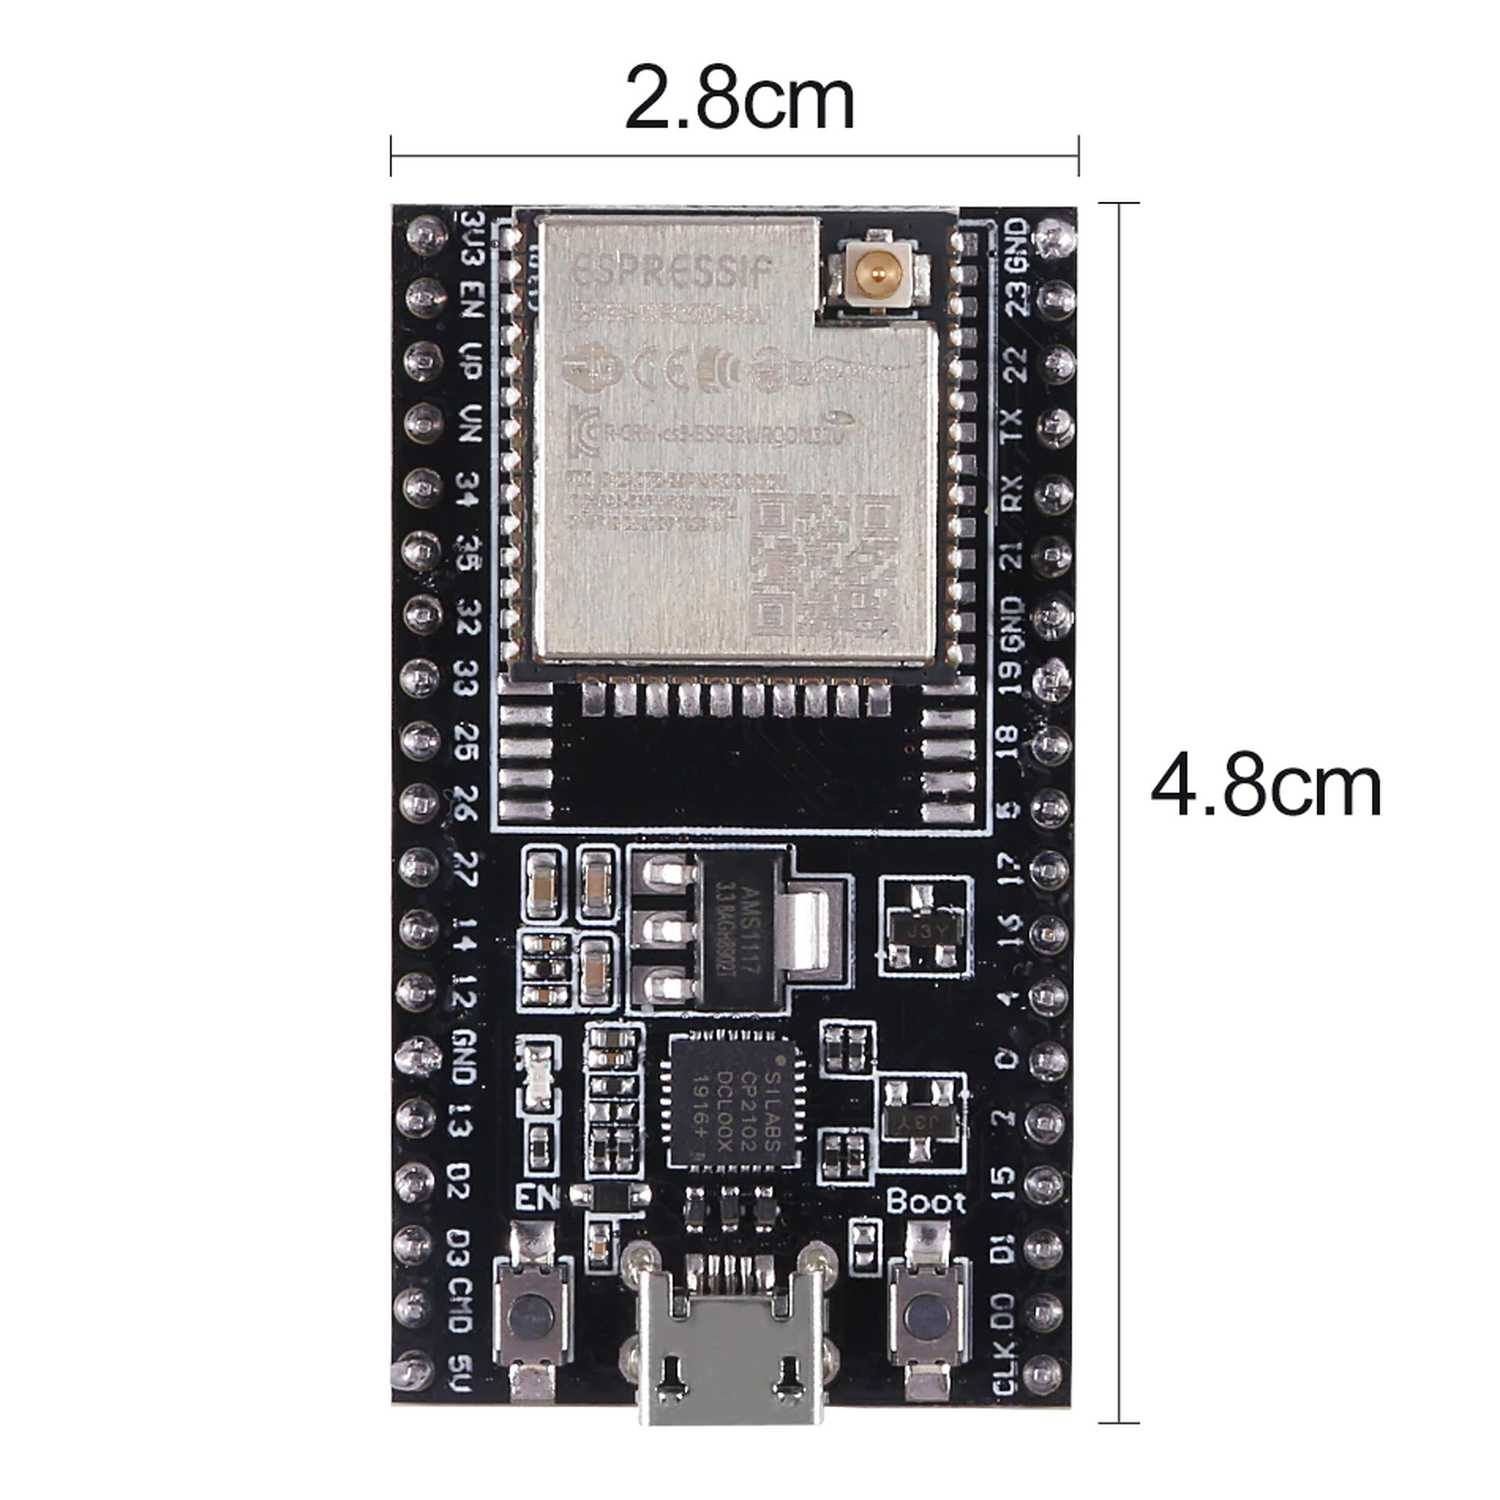
\includegraphics[width = 0.4\textwidth]{graphics/Produktbild_ESP32_2}
\caption{ESP32-32U DevKit.}
\label{fig:Produktbild_ESP32_32U_DevKit}
\end{figure}

\subsection{USB-B}
\label{subsec:USB-B}

Auf der Leiterplatte des PartyMixer's gibt es zwei Komponenten, welche programmiert werden müssen. Der Mikrocontroller und das WiFi-Modul. Um diese zu programmieren braucht es eine entsprechende Schnittstelle, welche mit einer USB-B-Schnittstelle realisiert wird.

Die USB-B-Schnittstelle benötigt nur zwei Kommunikationsleitungen (D+ und D-). Die zu programmierenden Komponenten (ESP32 und ATMega2560) benötigen zusätzliche Steuerleitungen um in einen Programmiermodus zu kommen und statt einem differenziellen Verfahrens ein serielles Verfahren. Deswegen benötigt es einen USB-UART-Converter.

Die beiden Kommunikationsschnittstellen (ATMega2560 und ESP32) benötigen unterschiedlich viele Steuerleitungen, da sie sich im Verfahren zum Aufruf des Download-Boot-Modus unterscheiden. In Tabelle \ref{tab:USB_uC} und \ref{tab:USB_ESP} wird dargestellt, welche Leitungen für das jeweilige Flash-Interface benötigt werden.
%Die USB-B-seitige Schnittstelle wird an den Computer angeschlossen und muss nicht häher betrachtet werden.

\begin{table}[h!]
\center
\begin{tabular}{|c|lcl|c|}
\hline
\textbf{Mikrocontroller} & & & & \textbf{USB-Flash-Device} \\ \hline
RX & <== & direkt & === & TX  \\
TX & === & direkt & ==> & RX  \\
Reset & <== & Kondensator & === & DTR \\
\hline
\end{tabular}
\caption{Verbindung zwischen USB und Mikrocontroller.}
\label{tab:USB_uC}
\end{table}

\begin{table}[h!]
\center
\begin{tabular}{|c|lcl|c|}
\hline
\textbf{ESP} & & & & \textbf{USB-Flash-Device} \\ \hline
RX & <== & direkt & === & TX  \\
TX & === & direkt & ==> & RX  \\
EN & <== & über Transistor & === & RTS \\
IO\_0 & <== & über Transistor & === & DTR \\
IO\_13 & <== & über Widerstand & === & RTS \\
IO\_15 & <== & über Widerstand & === & CTS \\
\hline
\end{tabular}
\caption{Verbindung zwischen USB und ESP.}
\label{tab:USB_ESP}
\end{table}

%Um in den automatischen Programmiermodus zu kommen, muss folgender Handshake zwischen den Geräten stattfinden:


%Auch hier wurde vom Arduino Uno-Board abgekpufert und der selbe Chip verwendet, um die USB-Signale in UART-Signale zu konvertieren. Das vorkommende Bauteil ist der CP2102N. Da dieser Chip ein TQFP-28-Gehause hat, könnte es auch schwierigkeiten geben beim Löten. Deswegen wird auch ein Breakout-Board (BOB) mitgeplant, damit es eine Ausweichmöglickeit gibt falls die Bauteile zu klein sind.

%\begin{figure}[!h]
%\center
%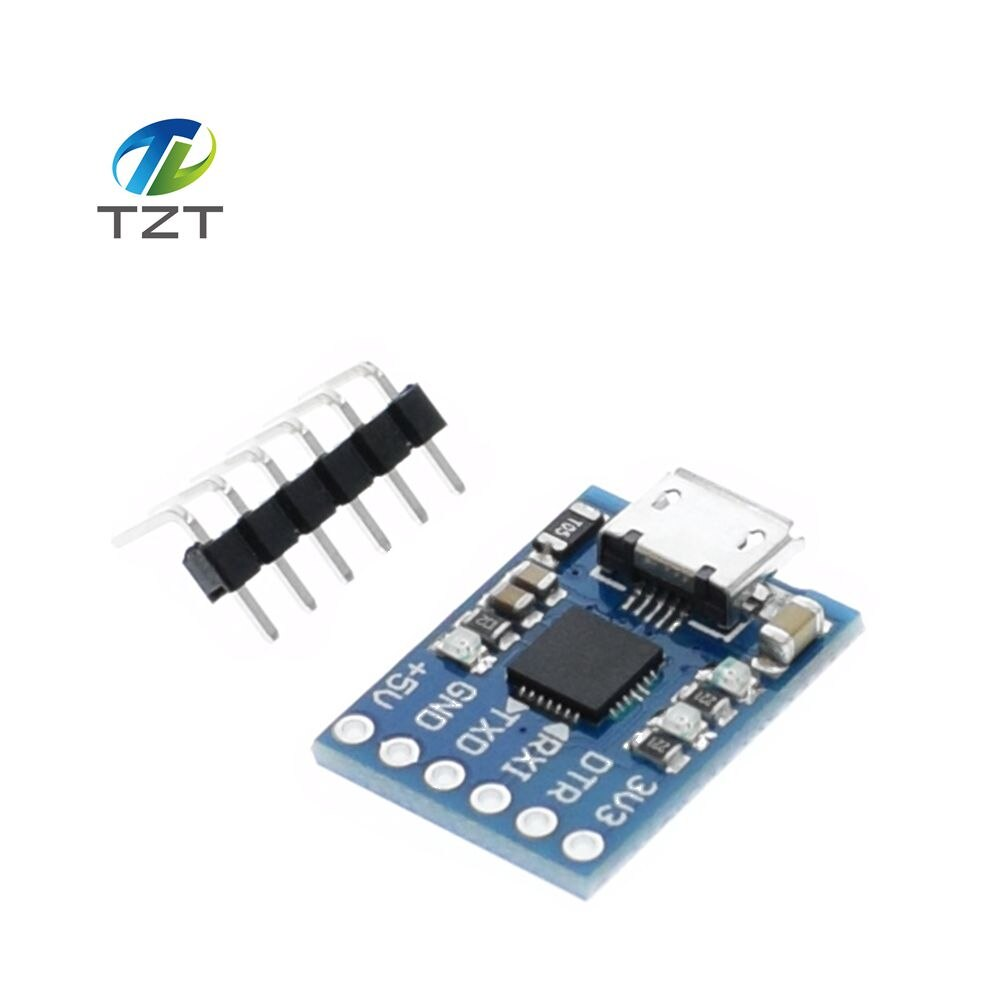
\includegraphics[width = 0.5\textwidth]{graphics/Produktbild_USB_UART_uC}
%\caption{CP2102N-BOB für uC.}
%\label{fig:Produktbild_USB_UART_uC}
%\end{figure}
%
%\begin{figure}[!h]
%\center
%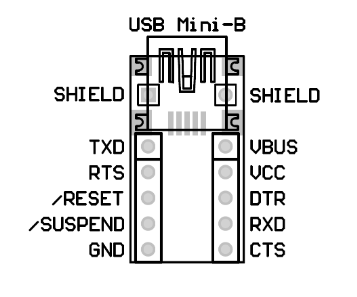
\includegraphics[width = 0.5\textwidth]{graphics/Produktbild_USB_UART_ESP}
%\caption{CP2102N-BOB für ESP.}
%\label{fig:Produktbild_USB_UART_ESP}
%\end{figure}
	
\subsection{RFID}
\label{subsec:RFID}

Eine vorgesehene Funktion der Maschine ist, dass der User ohne Suchen sein Lieblingsgetränk zubereiten lassen kann. Dafür wird auf ein System zurückgegriffen, was öfters für Zutrittskontrollen oder Ähnliches verwendet wird. Nämlich RFID \footnote{Radio Frequency IDentification}.

Um schnell ein funktionierendes Teilsystem testen zu können, soll ein Breakout-Board verwendet werden. Eine Recherche hat ergeben, dass es nicht allzu viele Produkte gibt. Ein Eingenzungskriterium war, dass es es für den Ausgewählten IC eine vorgeschriebene Library gibt, welche sich mit Arduino bewährt hat. Der Chip, welcher diese Anforderungen erfüllt, ist der \textbf{Mifare MFRC522}. Er ist in Abbildung \ref{fig:Produktbild_RFID_MFRC522} abgebidet. Dieses Brakeout-Board kann ausserdem an der Verschalung der Maschine angeschraubt werden. Somit kann er sich an einer Stelle befinden, welche weiter weg von der Hauptsplatine ist.
Das Modul arbeitet auf 13.56MHz und gilt somit als kurzwelliges System (HF).

Der MFRC522 ist der Reader im RFID-System. Er kann Daten lesen und ggf. auch schreiben. Er erzeugt ein hochfrequentes, elektromagnetisches Wechselsignal mit einer Frequenz von 13.56MHz. Der RFID-Tag wird von der Energie des Wechselsignals gespiesen. Durch Kurzschliessen der Tag-Antenne wird ein Teil der Energie des vom Reader ausgehenden Wechselfeldes verbraucht. Diese Energiedifferenz kann ein Reader detektieren. Die Reichweite für ein solches System beträgt weniger als 10cm.

Alternativ könnte ein Tag mit einer Batterie gespiesen werden. Somit erhöht sich die Reichweite des Readers, die Latenzzeiten werden kürzer und der Anwendungsbereich würde grösser.

%\begin{figure}[!h]
%\center
%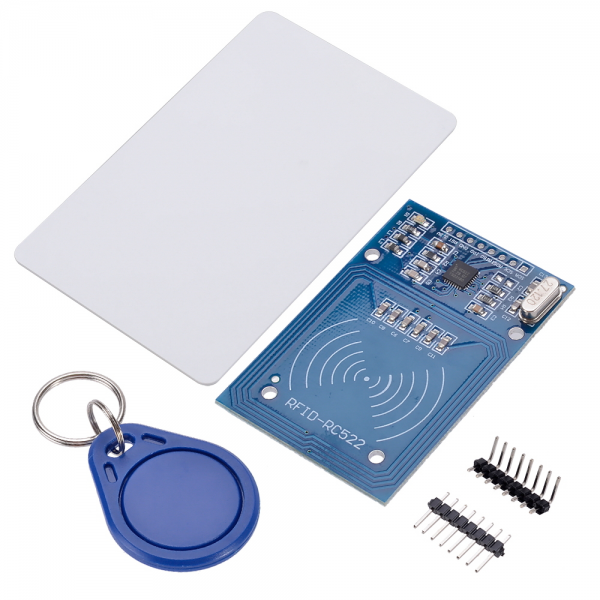
\includegraphics[width = 0.6\textwidth]{graphics/Produktbild_RFID_MFRC522}
%\caption{MFRC522.}
%\label{fig:Produktbild_RFID_MFRC522}
%\end{figure}



\subsection{SD-Karte}
\label{subsec:SD_Karte}

Damit gespeicherte Getränke, Zutaten und Maschinenzustände bei einem Neustart der Cocktailmaschine erhalten bleiben, werden diese auf der SD-Karte abgelegt. Nest dem Erhalten der Informationen ist die SD-Karte wichtig für den Betrieb der Maschine. Werden zu viel Getränke und Zutaten gespeichert, so führt dies zu einem Absturz des Mikrocontrollers. Es wurde entschieden, eine mikroSD zu verwenden. Im Folgenden wird erklärt, was es Hard- und Softwaretechnisch zu beachten gibt.

Abbildung \ref{fig:micro_sd_pinout} zeigt die Pinbelegung einer mikroSD-Karte. Es ist erkennbar, dass sie über SPI kommuniziert. Für den Anschluss wird nur ein mikroSD-Sockel benötigt. So kann die mikroSD über den Level-Shifter vom Mikrocontroller angesteuert werden.

\begin{figure}[h!]
	\centering
	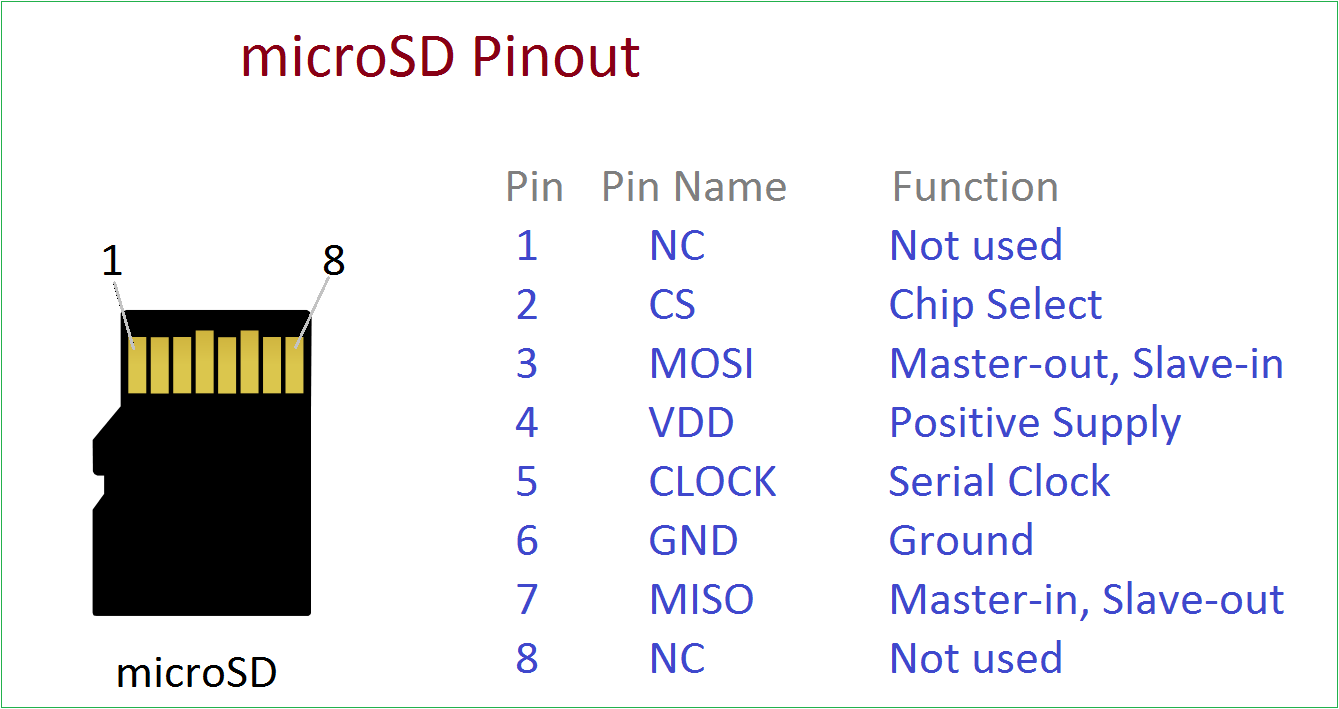
\includegraphics[width=0.55\textwidth]{graphics/micro-sd-pinout}
	\caption{Codeausschnitt aus dem Programmier-Tool. Auf diese Weise werden der DTR- und der RTS-Pin angesteuert während dem Programmiervorgang.}
	\label{fig:micro_sd_pinout}
\end{figure}

\todo{cite: https://www.ecosia.org/images?q=mikroSD+pinout\#id=F8E296D6DF751D79D199FC7711B8A9D178456B6F}

Als Dateisystem wird FAT32 verwendet. FAT32 steht für File Allocation Table mit 32Bit Datenbreite. Es ist ein von Micosoft entwickeltes System, dessen Wurzeln bis ins Jahr 1977 zurückreichen und heute noch der Industriestandard unter den Dateisystemen ist.

\todo{cite: https://www.ionos.de/digitalguide/server/knowhow/fat32/}

Der Speicherbereich einer FAT32-formatierten Partition besteht aus fünf Bereichen.
\begin{enumerate}
\item Master Boot Record (LBA Sektor 0 des Laufwerks)
\item Volume Boot Record, Partition Boot Sektor (LBA Sektor 0 der Partition)
\item File Allocation Table (i.d.R 2 mal hintereinander vorhanden, direkt nach dem PBR)
\item Directory Table (mit den Ordner und Fileeinträgen)
\item Datenbereich (Fileinhalt)
\end{enumerate}

\todo{cite: https://docplayer.org/78333139-Aufbau-des-fat32-dateisystems.html}

Im Master Boot Record ist ein Startprogramm vorhanden, welches für BIOS baseierte Computer geschrieben wurde.
Darin enthalten sind der Boot-Code in Assembler, Fehlermeldungen je nach Landessprache, Darstellungen der Fehlermeldungen, die Disk Signature, für die Organisation des Laufwerks wichtige Partitionstabelle und die Signature ID oder auch Magic Number 0x55 0xAA. Hier wird die aktive Partition ausgewählt und der Boot Sektor geladen. Da nicht über die SD-Karte gebootet wird, besteht dieser Teil nur aus Gründen der Kompatibilität.

\todo{cite: https://www.german-sales.com/datenstruktur.htm}

\todo{cite: https://docplayer.org/78333139-Aufbau-des-fat32-dateisystems.html}

Im Volume Boot Record befinden sich 3 Sektoren. Der erste Sektor enthält einen Sprungbefehl und einen ''tu nichts'' Befehl (''nop''), den Systemname (OEM ID), den BIOS Parameter Block, den Boot Code, der Bootloader File Name, Fehlermeldungen, Darstellung der Fehlermeldungen und ebenfalls die Magic Number 0x55 0xAA. Der zweite Sektor enthält den Anfang des erweiterten Volume Boot Records eines FAT32 Systems, den Anfang der Daten und das nächste verfügbare Cluster sowie die Magic Number. Hier kann kalkuliert werden, wieviel freier Speicher noch verfügbar ist. Der dritte Sektor ist eine Erweiterung des ersten Sektors, falls der Speicher für den Bootcode nicht ausreicht. Unter FAT32 wird für die drei Sektoren eine Sicherheitskopie abgelegt, welche zur Wiederherstellung des Volume Boot Records dient.

Im File Allocation Table wird organisiert, welche Cluster auf der Partition belegt oder frei sind und wo die Folgecluster eines Files sind. Die Clustergrösse kann selbst bestimmt werden und beträgt bei SD-Karten mit kleinen Dateien optimalerweise 512Bytes. Dies ist die minimale Grösse, da ein Cluster aus mehreren Sektoren besteht und ein Sektor 512 Bytes gross ist. Für die Cocktailmaschine weden pro File ca. 100 Bytes verwendet, wodurch pro File ca. 412 Bytes unnutzbar werden. Der Nachteil ist, dass die FAT so grösser wird und grosse Dateien mehr zerstückelt werden. Die Cluster sind fortlaufend nummeriert, wobei sich die Nummerierung in der FAT immer auf den Ort innerhalb der FAT bezieht, nicht auf den realen Ort auf der Partition. Ist ein File grösser als 512 Bytes, so ergibt sich eine Clusterkette, welche einen Verweis auf das nächste Cluster enthält und ein Verweis, falls die Kette zu ende ist. Jeder Eintrag der FAT ist 32 Bit lang (4 x 8 Bytes = 4 Doppelwörter). Ein Cluster kann z.B den Wert 0x0E 00 00 00 haben, wobei der Verweis 0E auf das nächste Cluster zeigt. Ein Endcluster ist mit dem Doppelwort 0xFF FF FF 0F gekennzeichnet. Ist eine Datei Fragmentiert, ist die Nummerierung nicht fortlaufend, sonder spring hin und her. Konklusion: Die Werte innerhalb des FAT zeigen an, ''wo sich relativ gesehen die Daten eines Files auf der Partition finden lassen. Dabei sind die Werte entweder das Zeichen für ein Clusterende oder sie zeigen auf den nächsten Cluster der Clusterkette innerhalb der FAT'' \todo{cite: https://docplayer.org/78333139-Aufbau-des-fat32-dateisystems.html}. Um jedoch das Anfangscluster auf der Partition finden zu können, muss das Directory Table angeschaut werden.

Im Directory Table sind alle Files und alle Ordner der Partition beschrieben. Der Startsektor errechnet sich aus der letzten FAT und der Grösse der FAT (Addition). In diesem Bereich befindet sich das Root Directory, oder auch Wurzelverzeichnis genannt. Es hat eine hiararchische Baumstruktur, was bedeutet, dass ''das Wurzelverzeichnis das oberste mögliche Verzeichnis ist unter dem sich weitere Verzeichnisse befinden können'' \todo{cite: https://docplayer.org/78333139-Aufbau-des-fat32-dateisystems.html}. Bis auf das Wurzelverzeichnis haben alle anderen Verzeichnisse ein einziges Elternverzeichnis, können aber mehrere Unterverzeichnisse haben.

\todo{cite: http://www.informatik.uni-ulm.de/ni/Lehre/WS01/TI2/folienmb/fat32slide.pdf}

\newpage
\subsection{Beleuchtung}
\label{subsec:Beleuchtung}

Damit die Maschine optisch etwas hergibt, wurde entschieden die ganze Maschinerie mit LED-Streifen zu verzieren. Dazu ist einerseits das LED-Band von nöten und die geeignete Ansterung dazu. Für die Cocktailmaschine wurde festgelegt, dass der LED-Streifen die benötigten Wirderstände für die LED's schon aufgeklebt hat und die Ansteuerung folglich direkt über FET's geschehen kann. Der Aufbau ähnelt dann dem in Abbildung \ref{fig:LED1} gezeigten Schaltung. Der Streifen wäre Rot eingerahmt, die LED's und Widerstände befinden sich auf dem Band und die zu sehenden Fähnchen für R, G, B und W führen zum Mikrocontroller. Es können auch mehrere Bänder parallel geschaltet werden, wie auf dem Bild.

\begin{figure}[h!]
\center
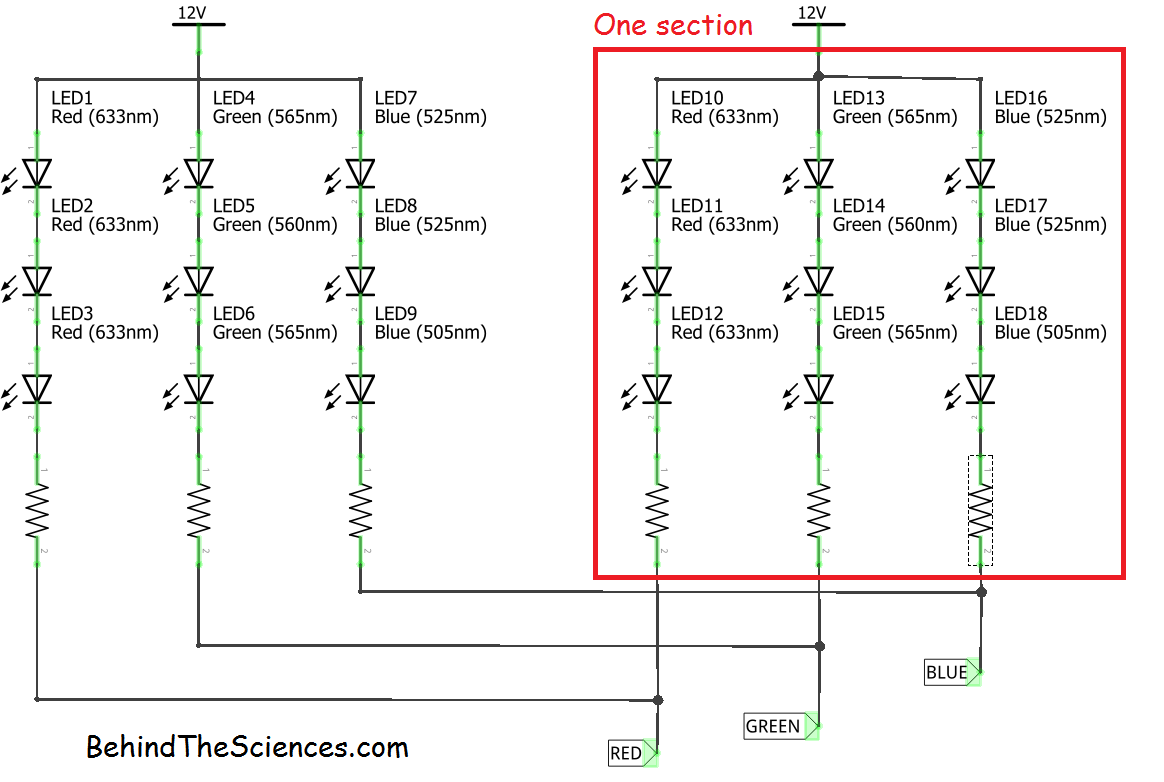
\includegraphics[width = 0.6\textwidth]{graphics/Schema_LED1}
\caption{LED Beispiel.}
\label{fig:LED1}
\end{figure}

\section{Printaufbau}
\label{sec:Printaufbau}



\newpage
\section{Teilsysteme}
\label{sec:Teilsysteme}

Da der Partymixer aus vielen kleineren und grösseren Teilsystemen besteht, werden diese in diesem Kapitel einzeln aufgelistet und im Detail angeschaut.
Es wird dabei bei jedem Teilsystem auf drei Punkte eingegangen, die Problemstellung (Was ist der Zweck der Teilschaltung und wesshalb wird sie benötigt?), das Schema und der Funktionsbeschrieb der Schaltung. Das komplette Schema kann in  \textcolor{red}{\textbf{Anhang Schema}} begutachtet werden.

\todo{Schema richtig Referenzieren und in Anhang machen}

\subsection{Speisungen}
\label{subsec:Speisungen}

Die Speisung, welche das System mit Strom versorgt, ist ein essentieller Bestandteil des PartyMixer's. Im System befinden sich vier verschiedene Speisungen auf verschiedenen Spannungsniveaus. Die Eingangsspannung, womit zwei andere Speisespannungen erzeugt werden und der Motor betrieben wird, wird von einem 48V Netzteil erzeugt. Mittels Step-Down Reglern wird aus der 48V Eingangsspannung eine 12V und eine 5V Speisung erzeugt. Bei der vierten Speisung handelt es sich um einen einfachen Linearregler, welcher aus den 5V eine 3.3V Speisung realisiert. In den folgenden Unterkapitel können die Details der einzelnen Spannungsquellen entnommen werden und deren Aufgabengebiet. Die Grundlage sämtlicher Berechnungen der 5V und 12V Speisungen sind dem Datenblatt entnommen \cite[S.10]{monolithic_power_systems_mp24943_2011}.

\subsubsection{48V Speisung}
\label{subsubec:48V Speisung}

\paragraph{Problemstellung}\mbox{}\\

Der Motor wird mit einer Spannung von 48V betrieben. Dies ist zugleich auch die höchste verwendete Speisespannung. Um diese Speisung gewährleisten zu können, wird ein fertiges Netzteil gemäss  \textcolor{red}{\textbf{Fachbericht 5}} eingesetzt.

\paragraph{Schema}\mbox{}\\

Es wurde im Projekt 5 entschieden, dass die 48V Speisung extern als fertiges Netzteil eingekauft wird. Somit entfällt das Schema für diesen Speisungsteil.  

\begin{figure}[h!]
	\centering
	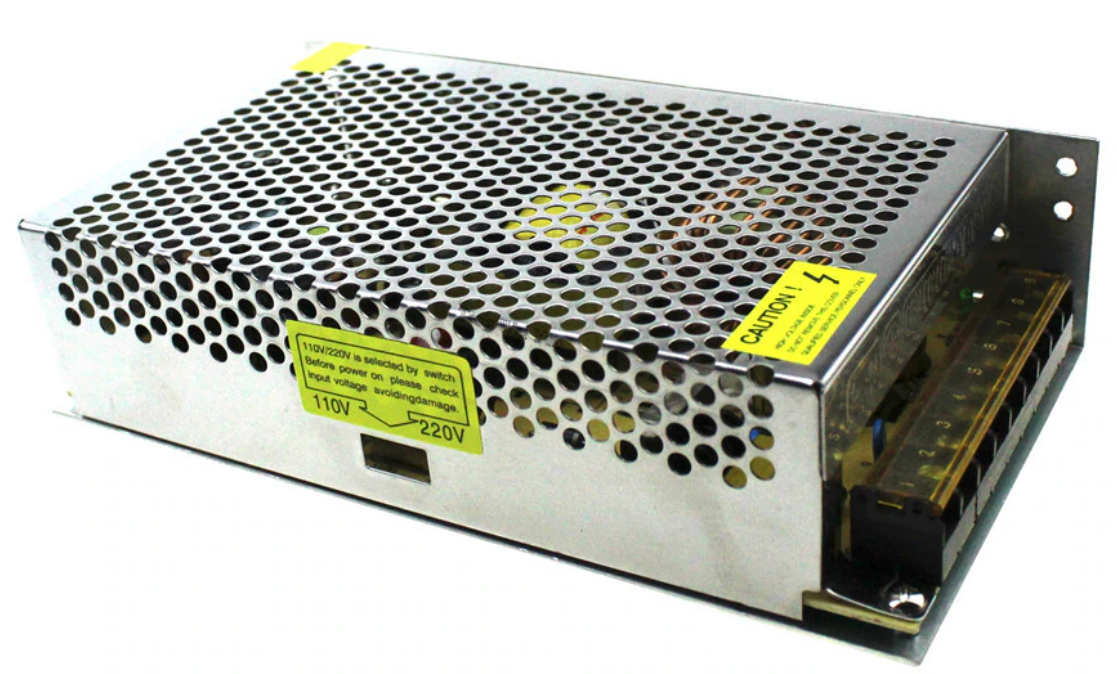
\includegraphics[width=0.8\textwidth]{graphics/Netzteil_48V.png}
	\caption{Anschauungsbild des 48V Netzteils}
	\label{fig:Netzteil_48V}
\end{figure} 


\paragraph{Funktionsbeschrieb}\mbox{}\\

Es musste jedoch unbedingt eine Leistungsabschätzung gemacht werden. Auch diese wurde im Projekt 5 durchgeführt. Unter Berücksichtigung der Schaltungsteile welche noch im Projekt 6 ergänzt werden, wurde dieses dann ausgewählt und eingekauft. Die Leistungsabschätzung kann im \textcolor{red}{\textbf{Fachbericht 5}} eingesehen werden. 

\subsubsection{12V Speisung}
\label{subsubsec:12V Speisung}

Die Pumpen werden mit 12V betrieben, was zur folge hat, dass eine 12V Speisung implementiert werden musste. Dazu wird ein Schaltspannungsregler verwendet. Dieser wandelt mittels Step-Down Prinzip die 48V des Netzteils in eine Konstantspannungsquelle von 12V. Es handelt sich hierbei um einen Regler von Monolithic Power Systems. Genauer gesagt um den MP24943DN-LF. Die Auswahl ist auf dieses Bauteil gefallen, da mit 48V eine relativ hohe Eingangsspannung verarbeitet werden muss. Der MP24943DN-LF kann am Eingang mit Spannungen von 4.5-55V arbeiten und dabei eine Ausgangsspannung von 0.8-45V erzeugen. Dies bei einem maximalen Strom von bis zu 3A. Die Realisierung der 12V Speisung kann in Abbildung \ref{fig:Schema_Speisung_12V} betrachtet werden.\\

\paragraph{Schema}\mbox{}\\

Das Schema in Abbildung \ref{fig:Schema_Speisung_12V} kann in fünf Teile unterteilt werden. Da wäre zuerst der Eingangsfilter, welcher mit C32, C34 \& C36 realisiert ist. Dieser Eingangsfilter wird gefolgt von einem Spannungsteiler, welcher den Enable auf aktiv setzt. Der eigentliche Regler wird mittels des IC7, D6 \& L3 realisiert. Mittels zweier Spannungsteiler, wird die gewünschte Ausgangsspannung, sowie die "Overvoltage-Protection" eingestellt. Vor dem Ausgang der Schaltung ist dann erneut eine Filterstufe implementiert, welche das Ausgangssignal glättet.

\begin{figure}[h!]
	\centering
	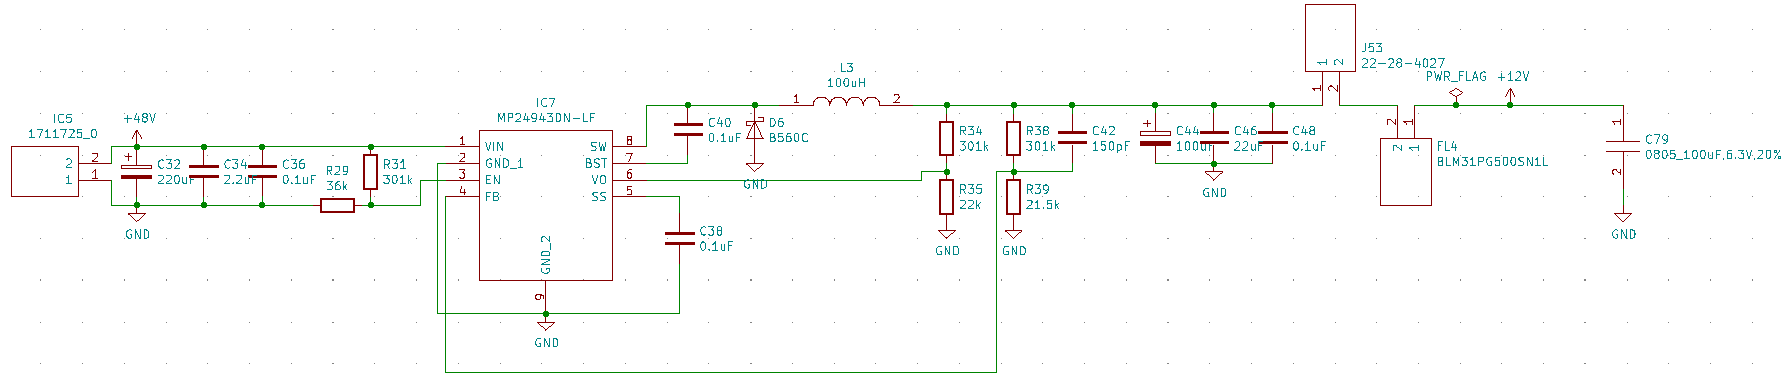
\includegraphics[width=\textwidth]{graphics/Schema_Speisung_12V.png}
	\caption{Schema der 12V Speisung}
	\label{fig:Schema_Speisung_12V}
\end{figure} 

\paragraph{Funktionsbeschrieb der Schaltung}\mbox{}\\

Um den MP24943DN-LF auf aktiv zu setzen, wird eine minimale Spannung von 1.8V vorausgesetzt. Fällt diese unter 0.4V, so wird dieser auf inaktiv gesetzt. Damit der Spannungsregler immer eingeschaltet ist, wird mittels zweier Widerstände R29 \& R31 ein Spannungsteiler realisiert, welcher den Enable (EN) Pin auf 5V und somit auf aktiv setzt. Dieser Spannungsteiler musste implementiert werden, da alle Eingangspins ausser dem V$_{in}$ einen maximale Eingangspegel von 6.5V verkraften können.

Die gewünschte Ausgangsspannung wird mittels Spannungsteiler R39 \& R40 eingestellt, welche auf den Feedback Eingang (FB) rückgekoppelt werden. Diese berechnet sich laut Datenblatt gemäss Formel \ref{equ:Ausgangsspannung_12V}. 

\begin{align}
R40 &= \frac{R39}{\frac{Vout}{0.8}-1}
\label{equ:Ausgangsspannung_12V}
\end{align}

Bei einem Widerstandsverhältnis von R39=301k$\Omega$ \& R40=21.5k$\Omega$ entspricht dies einer Ausgangsspannung von 12V.

Um einer Überspannung vorbeugen zu können, wird am Eingang Voltage-Overshoot (VO) ein Spannungsteiler implementiert. Diese wird am VO-Eingang mit einer Referenzspannung von 0.9V verglichen. Übersteigt die Spannung an VO die Referenzspannung von 0.9V, so wird der Regler ausgeschaltet, bis die Spannung wieder unter 0.9V fällt. Als maximale Ausgangsspannung wurde hierbei eine Spannung von 13V gewählt. Diese Wahl wurde getroffen, da die 12V ausschliesslich für die Ansteuerung der Pumpen verwendet wird und diese eine Spannung von 13V verkraften können ohne Schaden zu nehmen. Der Spannungsteiler wird gemäss Datenblatt mit der Formel \ref{equ:Vovp_12V} berechnet. 

\begin{align}
R35 &= \frac{R34}{\frac{Vovp}{Vovref}-1}
\label{equ:Vovp_12V}
\end{align}

Bei einem Widerstandsverhältnis von R34=301k$\Omega$ \& R35=22k$\Omega$ entspricht dies einer Überspannungsschutzschwelle von 13.21V. 

Der Rippel des Spulenstroms lässt sich gemäss Formel \ref{equ:12V_Spulenberechnung} berechnen. Dieser sollte gemäss Datenblatt ca. 30\% des maximalen Ausgangsstroms von 3A betragen. 

\begin{align}
L3 &= \frac{Vout \cdot (Vin-Vout)}{Vin \cdot \Delta IL \cdot fosc}
\label{equ:12V_Spulenberechnung}
\end{align}

Der interne Oszillator läuft dabei bei einer Frequenz von 100kHz. Bei der ausgewählten Spule von 100$\mu$H erhalten wir ein $\Delta$I$_{L}$ von 0.9A. Ausserdem wird im Datenblatt darauf hingewiesen, dass die gewählte Spule auf mindestens 125\% des maximalen Ausgangsstroms von 3A ausgelegt werden soll. Auch der Gleichstromwiederstand der Spule sollte $ \leq \ $ 200m$\Omega$  sein. 

Mit den Kondensatoren C45, C47 \& C49 wird die Ausgangsspannung zum Abschluss noch geglättet. Bei den Eingangskondensatoren, sowie den Ausgangskondensatoren sollte es sich um low ESR Typen handeln. Um die restlichen hochfrequenten Störungen herauszufiltern, ist zum Abschluss ein Ferrit implementiert worden.

Um die Schaltung einfacher in Betrieb nehmen zu können, wurde mittels Jumper sichergestellt, dass die Speisung vom System abgekoppelt werden kann. Ein LED zeigt an, ob die Speisung funktioniert oder nicht. So ein LED ist jeweils vor und nach dem Jumper implementiert worden. Der Ferrit FL2 soll noch letzte Störungen herausfiltern.



\subsubsection{5V Speisung}
\label{subsubsec:5V Speisung}

Der Mikrocontroller, sowie die Durchflussmessgeräte und das Display  werden mit 5V betrieben. Aus diesem Grund wurde eine 5V Speisung implementiert. Dazu wird der selbe Schaltspannungsregler wie bei der 12V Speisung in Kapitel \ref{subsubsec:12V Speisung} verwendet. Die Realisierung der 5V Speisung kann in Abbildung \ref{fig:Schema_Speisung_5V} betrachtet werden.\\

\paragraph{Schema}\mbox{}\\

Das Schema in Abbildung \ref{fig:Schema_Speisung_5V} kann wie bei der 12V Speisung gemäss Kapitel \ref{subsubsec:12V Speisung}in fünf Teile unterteilt werden. Da wäre zuerst der Eingangsfilter, welcher mit C31, C33 \& C35 realisiert ist. Dieser Eingangsfilter wird wiederum gefolgt von einem Spannungsteiler, welcher den Enable auf aktiv setzt. Der eigentliche Regler wird auch hier mittels des IC6, D5 \& L4 realisiert. Mittels zweier Spannungsteiler, wird die gewünschte Ausgangsspannung, sowie die "Overvoltage-Protection" eingestellt. Vor dem Ausgang der Schaltung ist dann erneut eine Filterstufe implementiert, welche das Ausgangssignal glättet.

\begin{figure}[h!]
	\centering
	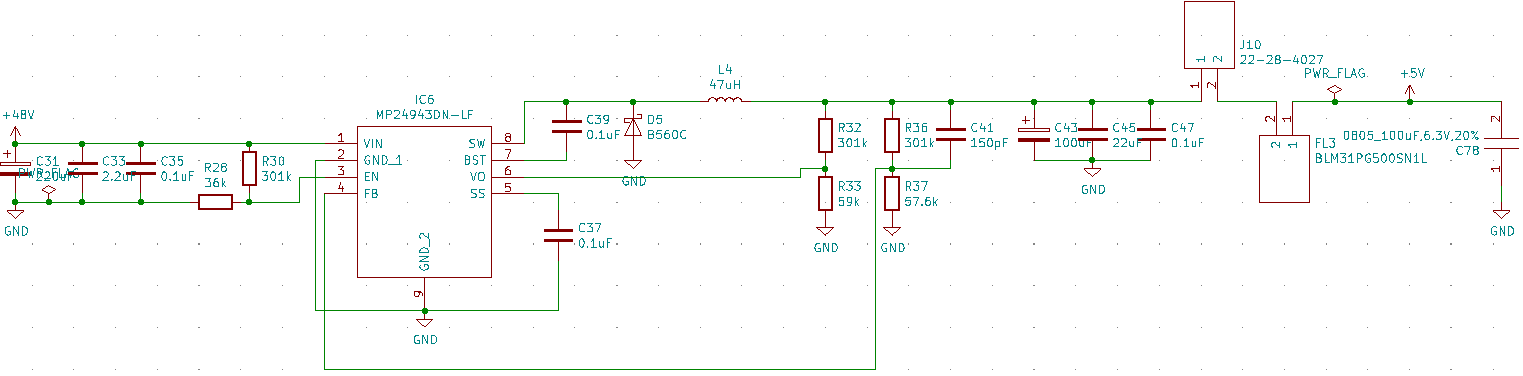
\includegraphics[width=\textwidth]{graphics/Schema_Speisung_5V.png}
	\caption{Schema der 5V Speisung}
	\label{fig:Schema_Speisung_5V}
\end{figure} 

\paragraph{Funktionsbeschrieb der Schaltung}\mbox{}\\

Auch bei der 5V Speisung wurde mittels R29 \& R31 ein Spannungsteiler realisiert, welcher das IC gemäss Kapitel \ref{subsubsec:12V Speisung} auf aktiv setzt.

Das Widerstandsverhältnis von R41 \& R42, welches die Ausgangsspannung definiert, wurde gemäss Formel \ref{equ:Ausgangsspannung_12V} berechnet. Somit ergeben sich für R41=301k$\Omega$ und für R42=57.6k$\Omega$, Was einer Ausgangsspannung von 4.98V entspricht. 

Beim Überspannungsschutz musste darauf geachtet werden, dass der Mikrokontroller AtMega2560-16AU nur in einem Spannungsbereich von 4.5V-5.5V betrieben werden darf. Die maximal verträgliche Eingangsspannung liegt laut Datenblatt bei 6V. Somit muss der Überspannungsschutz so gestaltet werden, dass die Schwelle von 6V nicht überschritten werden kann. Um dies erreichen zu können, wurde für R36=301k$\Omega$ und R37=53k$\Omega$ gewählt. Gemäss Formel \ref{equ:Vovp_12V} erhält man so eine Überspannungsschutzschwelle von 6V. 

Der interne Oszillator läuft wiederum bei einer Frequenz von 100kHz. Bei der ausgewählten Spule L4 von 47$\mu$H erhält man mittels Formel \ref{equ:12V_Spulenberechnung} ein $\Delta$I$_{L}$ von 0.953A. Auch hier gilt gemäss Datenblatt, dass die gewählte Spule auf mindestens 125\% des maximalen Ausgangsstroms von 3A ausgelegt werden soll. Auch der Gleichstromwiederstand der Spule sollte $ \leq \ $ 200m$\Omega$  sein. 

Mit den Kondensatoren C46, C48 \& C50 wird die Ausgangsspannung zum Abschluss auch noch geglättet. Bei den Eingangskondensatoren, sowie den Ausgangskondensatoren sollte es sich um low ESR Typen handeln. Auch hier wurde noch zum Abschluss ein Ferrit implementiert, welcher allfällige hochfrequente Störungen herausfiltern soll.

Auch bei der 5V Speisung wurde ein Jumper zu Testzwecken und zwei LED's implementiert. Ausserdem findet sich auch hier wieder ein Ferrit FL3, welcher letzte Störungen beseitigen soll. 




\subsubsection{3.3V Speisung}
\label{subsubsec:3.3V Speisung}

Um die Treiber der Motorenansteuerung, das Wireless-/Bluetoothmodul, die SD-Karte und die RFID-Schaltung zu betreiben, wird zusätzlich eine 3,3V-Speisung verbaut. Da es sich dabei nicht um  Leistungstreibende Elemente handelt, genügt ein einfacher Linearregler, der von der 5V-Speisung aus betrieben wird. 

\paragraph{Schema}\mbox{}

Bei dem Linearregler handelt es sich konkret um den LF33CDT-TRY von STMicroelectronics. Dieser hat eine fixe Ausgangsspannung von 3.3V bei einem maximalen Strom von 1A. Das dazugehörige Schema kann in Abbildung \ref{fig:Schema_Speisung_3.3V} begutachtet werden.

\begin{figure}[h!]
	\centering
	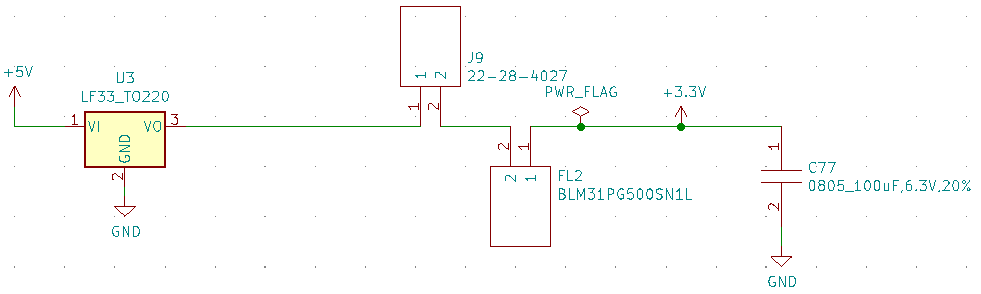
\includegraphics[width=0.5\textwidth]{graphics/Schema_Speisung_3,3V.png}
	\caption{Schema der 3.3V-Speisung}
	\label{fig:Schema_Speisung_3.3V}
\end{figure} 


\paragraph{Funktionsbeschrieb der Schaltung}\mbox{}

Der Linearregler benötigt keine spezielle Beschaltung. Er wird lediglich an die 5V Speisung angeschlossen. Am Eingang und am Ausgang ist ein Entstörkondensator implementiert. 

Wie bei der 12V-Speisung in Kapitel \ref{subsubsec:12V Speisung} und der 5V-Speisung in \ref{subsubsec:5V Speisung} wurde ein Jumper, sowie zwei LED's implementiert. Ein Ferrit FL1 filtert letzte Störungen heraus.

\clearpage
\subsection{Motor}
\label{subsec:Motor}

Um ein Glas während der Zubereitung hin- und her zu bewegen, wird eine Antriebsgruppe benötigt. Die Auswahl der Motorengruppe wurde mit dem Dozenten ausgewählt. Der Entscheid fiel dabei auf den Brushless DC-Motor AKM22h von Sigmatec. Auch dessen Ansteuerung ergab sich durch die schon vorhandenen EVAL-Boards mit dem FOC-Treiber (TMC4671) und der universal H-Brücke (UPS 10A70V). Im Projekt 6 wird anstelle der universellen H-Brücke ein Gate-Treiber (TMC6200) verwendet, welcher gemäss Kapitel \ref{subsubsec:Gate-Treiber} diverse Vorzüge hat. Das benötigte Feedback über die Lage des Rotors wird vom ABN-Encoder (AMT332S-V) geliefert. Zwei Shunts geben Auskunft über die Bestromung der Spulen. Auf die erwähnten Komponenten wird im Folgenden eingegangen. Abbildung \ref{fig:Blockdiagramm_TMC4671_und_TMC6200} zeigt, wie die Komponenten zusammenhängen.

\begin{figure}[H]
	\centering
	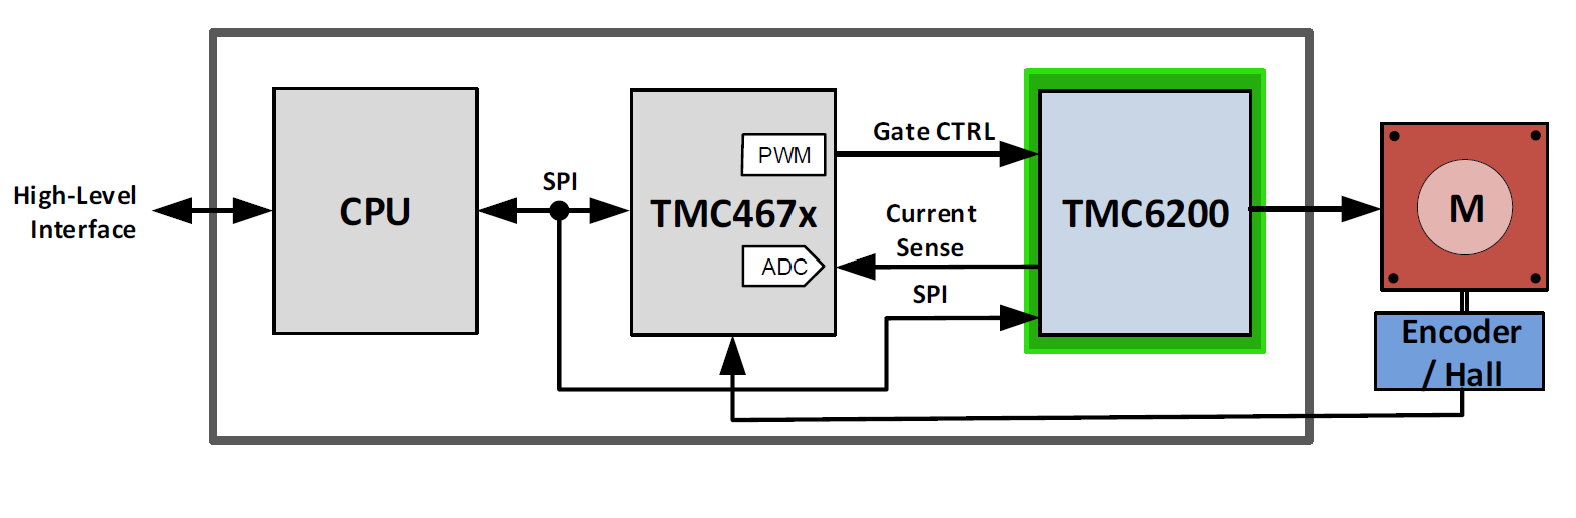
\includegraphics[width=0.8\textwidth]{graphics/Blockdiagramm_TMC4671_und_TMC6200}
	\caption{Blockschaltbild Konfiguration IC's mit BLDC und Encoder. \cite[S.1]{trinamicmotion_control_gmbh__co_kg_tmc6200_2019}}
	\label{fig:Blockdiagramm_TMC4671_und_TMC6200}
\end{figure}

%Es wurde darauf geachtet, dass der Aufbau des Prints dem Testaufbau entspricht. In Abbildung \ref{fig:Blockdiagramm_Motorengruppe} wird ein detaillierteres Blockschaltbild gezeigt, welches den Aufbau eher nach Funktionen beschreibt.

%\begin{figure}[H]
%	\centering
%	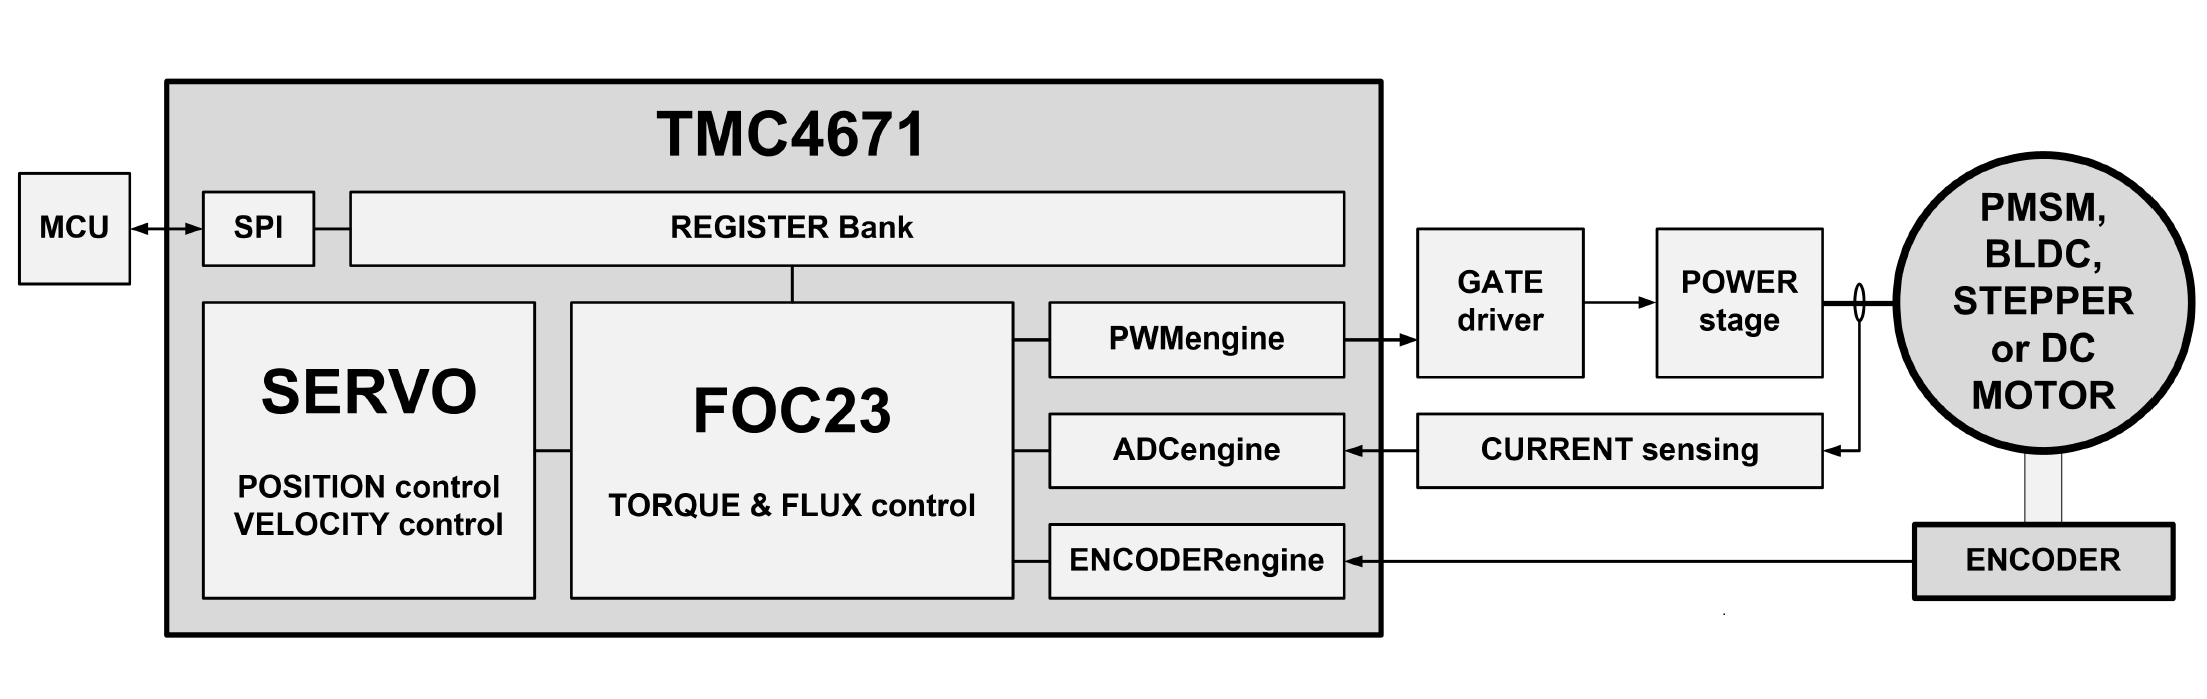
\includegraphics[width=0.8\textwidth]{graphics/Blockdiagramm_Motorengruppe}
%	\caption{Blockschaltbild Motorengruppe nach Funktionen. \cite[S.1]{trinamicmotion_control_gmbh__co_kg_tmc4671_2019}}
%	\label{fig:Blockdiagramm_Motorengruppe}
%\end{figure}

%\begin{table}[H]
%\center
%\begin{tabular}{|lll|l|}
%\hline
%\textbf{Kennzeichnung} & & \textbf{Bauteil} & \textbf{Funktion} \\
%\hline
%TMC4671 & = & Trinamic TMC4671 & FOC-Treiber \\
%GATE driver & = & Trinamic TMC6200 & Gate-Treiber \\
%POWER stage & = & Trnamic UPS 10A70V & H-Brücke \\
%Current sensing & = & UPS 10A70V ==> TMC6200 & Messung Phasenströme \\
%PMSM/BLDC & = & Sigmatec AKM22h & BLDC \\
%ENCODER & = & CUI devices ATS33 & ABN-Encoder \\
%\hline
%\end{tabular}
%\end{table}
%\newpage

\subsubsection{BLDC}
\label{subsubsec:BLDC}

Ein Brushless DC-Motor\footnote{Bürstenloser Gleichstrommotor} (BLDC) zeichnet sich dadurch aus, dass der Rotor mit Permanentmagneten bestückt ist. Somit ähnelt er vom Aufbau her einer Synchronmaschine mit permanent erregten Rotorwicklungen. Zur Ansteuerung hat der BLDC drei Phasenleitungen, die auf die Spulen führen. Die Spulen sind innerhalb des BLDC in Stern geschaltet. Der Motor hat drei Polpaare, womit die magnetische Winkelgeschwindigkeit drei Mal schneller ist als die mechanische.
%Ein Nachteil von BLDC-Motoren ist, dass bei Drehgeschwindigkeiten über Nenndrehzahl nur mit einer geeigneten Regelung der Statorwicklungen in Feldschwächung gefahren werden kann, anstelle dass der Erregerstrom verringert wird. Ansonsten zeichnet sich ein BLDC durch ein besseres Leistungs-/Gewichtsverhältnis aus als herkömmliche Motoren.

\paragraph{Schema}\mbox{}

Zum BLDC gibt es kein Schema. Die Anschlusspins für die Motorleitungen sind in Abbildung \ref{fig:Schema_H_Bruecke_und_BLDC} zu sehen.

\paragraph{Funktionsbeschrieb der Schaltung}\mbox{}

Im Folgenden werden die Eigenschaften des verwendeten BLDCs aufgelistet. So wurde beispielsweise die Versorgungsspannung nach der Nennspannung $V_M$ ausgewählt, das Limit des Geschwindigkeitsregelkreis auf 1500min$^{-1}$ gesetzt, der Strom auf 5A begrenzt \cite[S.36]{akm_servomotoren_2020}

\begin{table}
\begin{tabularx}{\textwidth}{|lllllX|}
\hline
\textbf{Beschreibung} & \textbf{Var} & & \textbf{Wert} & \textbf{Einheit} & \textbf{Benötigt für} \\
\hline
Nennnetzspannung & $V_M$ & = & 48 & [V] & Versorgungsspannung\\
Stillstanddrehmoment & $M_0$ & = & 0.88 & [Nm] & -\\
Nenndrehmoment & $M_n$ & = & 0.85 & [Nm] & -\\
Spitzendrehmoment & $M_{max}$ & = & 2.8 & [Nm] & -\\
Nenndrehzahl & $n_n$ & = & 1500 & [min$^{-1}$] & Limit: Geschwindigkeit (PI-Regler)\\
Nennleistung & $P_n$ & = & 0.13 & [kW] & Power Management\\
Stillstandstrom & $I_0$ & = & 5.41 & [A] & -\\
Nennstrom & $I_N$ & = & 5.21 & [A] & Limit: Strom (PI-Regler)\\
Spitzenstrom & $I_{max}$ & = & 21.6 & [A] & -\\
Drehmomentkonstante & $k_T$ & = & 0.1632 & [Nm/A] & Reglerauslegung\\
Rotorträgheitsmoment & $J$ & = & 0.16 & [kg$\cdot$cm$^2$] & Reglerauslegung\\
Gewicht & $m$ & = & 1.1 & [kg] & Mechanik\\
\hline
\end{tabularx}
\caption{Charakteristische Eigenschaften des BLDC}
\end{table}


\subsubsection{H-Brücke}
\label{subsubsec:H-Brücke}

Das Bindeglied zwischen Kraft (Motor) und Steuersignalen wird von der H-Brücke gebildet. Durch Laden-/Entladen der MOSFET-Gates wird die Spannung am Motor kommutiert.

\paragraph{Schaltungsaufbau}\mbox{}

Für den Aufbau und die Dimensionierung wurde das Referenzschema des Evaluationsboard verwendet, welches schon im Projekt 5 zum Einsatz gekommen ist (Trinamic UPS 10A70V) \cite{trinamicmotion_control_gmbh__co_kg_tmc-ups-xaxv-eval_2017}.  Das Schema ist im Anhang Kapitel \ref{Appendix:H_Bruecke_Referenzschema} zu finden. Die Dimensionierung der Shunts wurde in Kapitel \ref{subsubsec:Gate-Treiber} abgehandelt.

Der Schltungsaufbau ergibt sich durch den dreiphasigen Aufbau des BLDCs. Es werden so drei Stränge gebildet, woran jeweils eine Spule verbunden wird. Der Energiefluss führt dabei über einen Strommesswiderstand. Die Eingänge der H-Brücke werden zusätlich mit Stützkondensatoren bestückt, um eine saubere 48V-Netzspannung zu gewährleisten.

\begin{figure}[H]
	\centering
	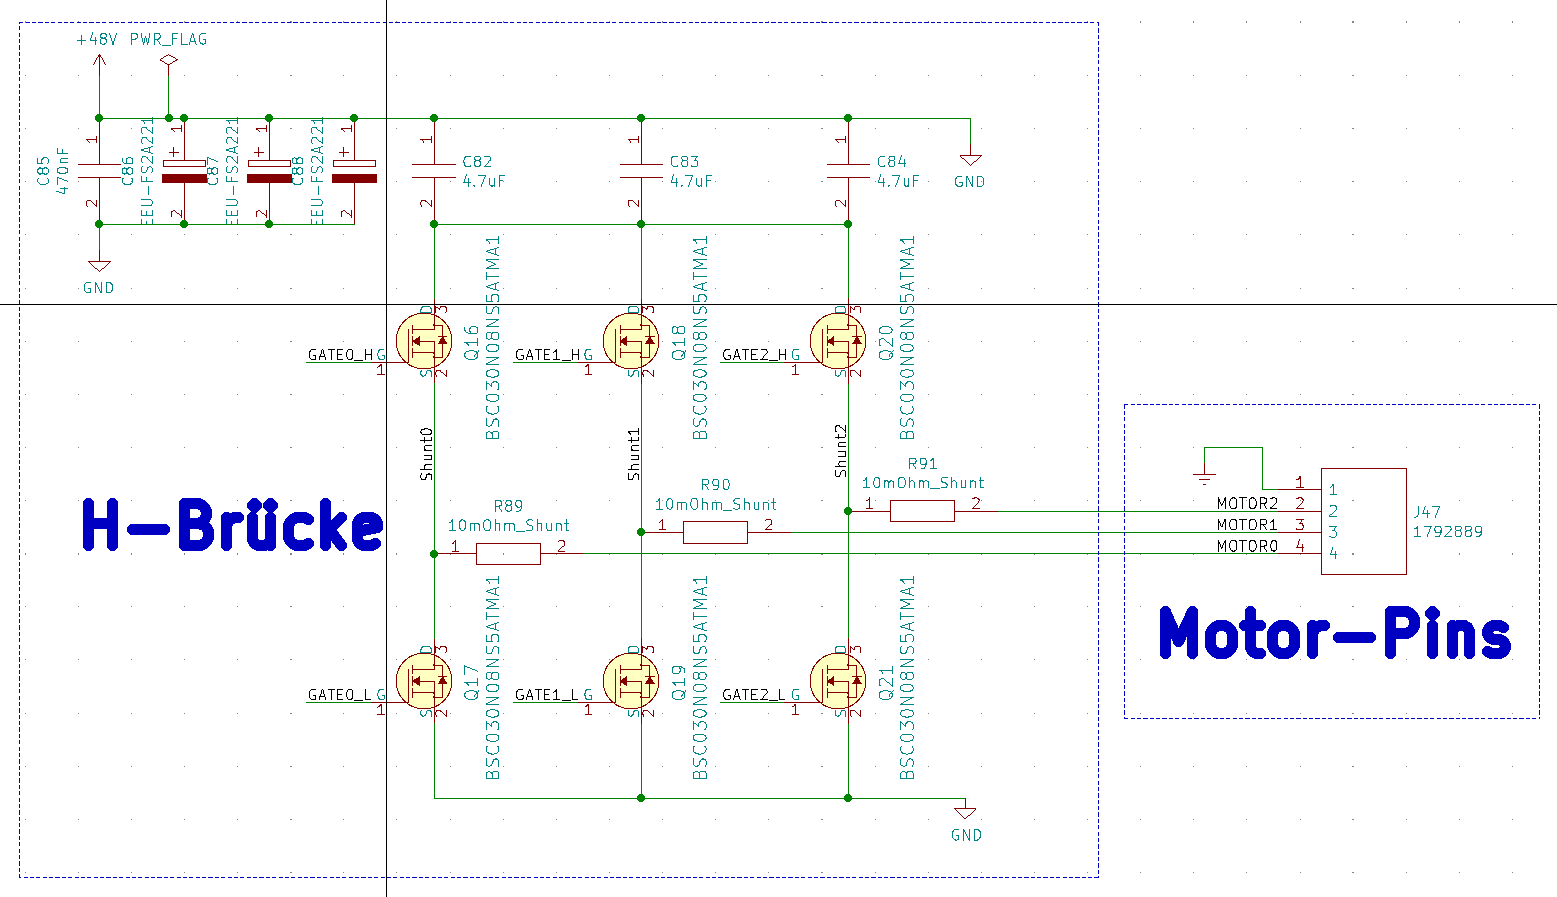
\includegraphics[width=\textwidth]{graphics/Schema_H_Bruecke_und_BLDC}
	\caption{H-Brücke.}
	\label{fig:Schema_H_Bruecke_und_BLDC}
\end{figure}

\paragraph{Funktionsbeschrieb der Schaltung}\mbox{}

Die Eingangsspannung der gesamte H-Brücke wird mit den Kondensatoren C85-C88 gestützt.
Bei C86-C88 handelt sich um Low-ESR Stützkondensatoren, jeweils ein Kondensator pro Phase.

Die Kondensatoren C82-C84 sind Kondensatoren, welche direkt zwischen Ein- und Ausgang eines H-Brücken-Strangs, nahe der MOSFETs platziert wurden.
Sie dienen auch zur Erhaltung der 48V-Versorgungsspannung.

Die MOSFETS Q16-Q21 bilden die eigentliche H-Brücke. Sie Schalten den Leistungsfluss gemäss den Gate-Ctrl-Signalen. Sie sind für 100A Nennstrom und 100V Sperrspannung ausgelegt. Die Gate-Source-Spannung beträgt $\pm$20V.

\subsubsection{ABN-Encoder}
\label{subsubsec:ABN-Encoder}

Für eine Geschwindigkeits- und Positionsregelung ist ein Positionsgeber unabdingbar. Diese Aufgabe übernimmt ein ABN-Encoder, welcher dem FOC-Treiber mittels digitalen Signalen die Positionsänderung in kleinen Schritten mitteilt. Die absolute Position wird vom FOC-Treiber berechnet. Gewählt wurde der AMT332S-V, weil er unempfindlich auf Staub, Schmutz und Öl ist, und weiler einfach zu montieren ist. Als Feature hat er eine über UART einstellbar hohe Genauigkeit, auf welche beim Funktionsbeschrieb eingegangen wird.

\paragraph{Schema}\mbox{}

Nebst der 5V-Spannungsversorgung sind die Signalleitungen (A, B und N) auf den Encoder geführt. Die Leitungen gehen auf den FOC-Treiber. Dies ist im Schema des FOC-Treibers zu sehen, welches in Abbildung \ref{fig:Schema_FOC_Treiber} dargestellt ist. Während A und B die Codierung für die relative Wegänderung sind, gibt N an, sobald eine gesamte Umdrehung erfolgte. Auf die Schaltung innerhalb des Encoders wird nicht weiter eingegangen.

\paragraph{Funktionsbeschrieb der Schaltung}\mbox{}

Die einstellbar hohe Genauigkeit zeigt sich in Form der Bitanzahl pro Umdrehung. Die maximale Auflösung liegt bei 4096 Schaltvorgänge pro Umdrehung, was einer Auflösung von 12 Bit entspricht. Der Encoder ist defaultmässig mit diesem Wert initialisiert und wird nicht verändert. Die Auflösung ist wichtig für die Implementierung in den FOC-Treiber. Die Auflösung bezieht sich auf eine Signalleitung. Für den FOC-Treiber entspricht dies einer gesamten Auflösung von 8192 Schaltvorgängen pro Umdrehung (A \& B = 2 $\cdot$ 4096Bits). Die Ausgangspins sind normale Header-Pins. Der Spannungsausgang wurde mit einem Stützkondesator C89 versehen um die Versorgungsspannung zu glätten. \cite[S.1]{cui_devices_cui_2019}

%\begin{figure}[h!]
%	\centering
%	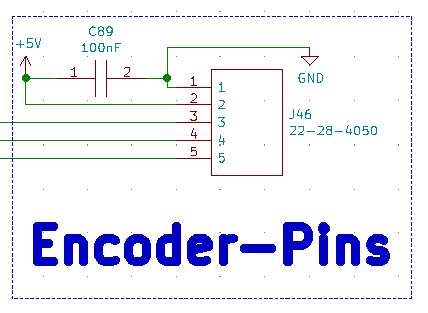
\includegraphics[width=0.5\textwidth]{graphics/Schema_ABN_Encoder}
%	\caption{Schema ABN-Encoder.}
%	\label{fig:Schema_ABN_Encoder}
%\end{figure} 

\clearpage
\subsubsection{FOC-Treiber TMC4671}
\label{subsubsec:FOC-Treiber_TMC4671}

Wie dem Grobkonzept in Kapitel \ref{subsec:Blockschaldbild} entnommen werden kann, wird für die Ansteuerung des BLDC-Motors eine Steuerlogik (Motor Control Unit) benötigt. Dabei handelt es sich um den TMC4671.
Der FOC-Treiber berechnet den Modulationsindex für die H-Brücke anhand des Drehmoments, der Geschwindigkeit oder der Position, welche der Mikrocontroller dem FOC-Treiber vorgibt. Die vom FOC-Treiber ausgehenden PWM-Leitungen gehen direkt auf den Gate-Treiber, welcher dann wiederum die MOSFETs ansteuert. Als Feedback benötigt der FOC-Treiber zwei Phasenströme. Der dritte Strom wird mit dem Knotengesetz berechnet. Da der BLDC in Stern geschaltet ist gilt:
\begin{equation}
I_U + I_V + I_W = 0
\end{equation}
Auf den FOC-Treiber und weitere für diesen Schaltkreis benötigte Komponenten wird im folgenden eingegangen.
Da das Gehäuse des IC's nur schwierig lötbar ist, wird ein Breakout-Board (BOB) verwendet.
Auf dem Board sind die Eingänge des FOC-Treibers schon geschützt mit Filtern und Überspannungsdioden. Somit entfällt eine Dimensionierung der Filter und Schutzschaltungen. Es wird jedoch die jeweilige Funktion der Schaltung beschrieben.

\paragraph{Schema}\label{par:Schaltungsaufbau_TMC4671}\mbox{}

Auf dem Breakout-Board sind diverse Anschlussmöglichkeiten vorhanden. Für den Cocktailmixer werden folgende Schnittstellen verwendet:

\begin{itemize}
\item SPI Input
\item Phasenströme Input
\item Encoder Input
\item Motorspannung Input
\item Steuersignale Output
\end{itemize}

Im Anhang \ref{Appendix:TMC4671} zeigt Abbildung \ref{fig:Blockdiagramm_TMC4671} anhand eines Blockdiagramms, welche Funktionen im Treiber vorhanden sind und wie diese zusammenhängen. Im wesentlichen kann daraus entnommen werden, dass der TMC4671 aus einer FOC-Logik\footnote{FOC= \textbf{F}ield \textbf{O}riented \textbf{C}ontrol}, einer Servo-Logik, einem SPI-Interface und diversen Engines (PWM, ADC, Encoder) besteht. In Abbildung \ref{fig:Schaltung_TMC4671} wird eine Standard-Anwendungsschaltung gezeigt, worin erkennbar ist, dass der Treiber sehr universell aufgebaut ist und für mehrere Motorentypen verwendet werden können.

\begin{figure}[h!]
	\centering
	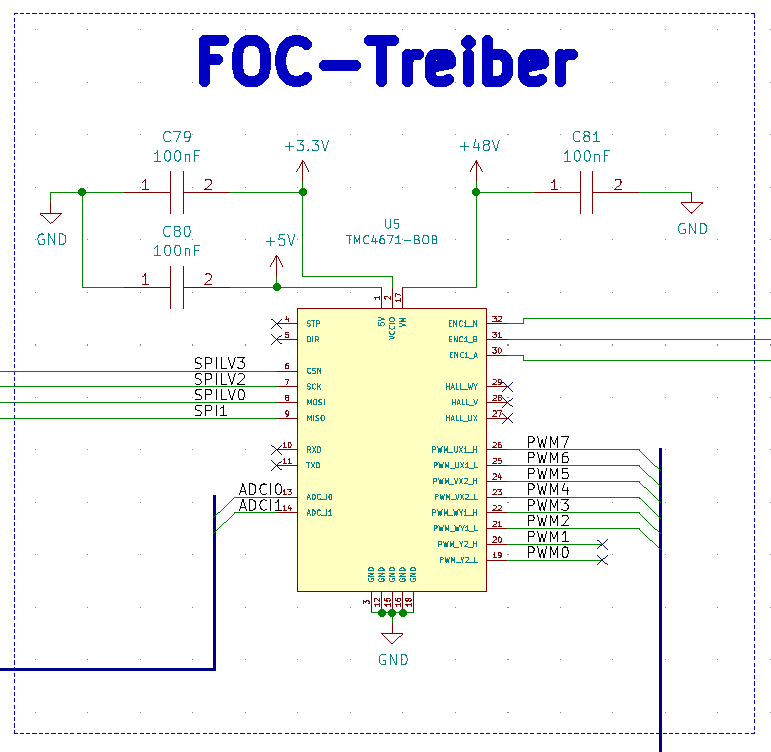
\includegraphics[width=0.5\textwidth]{graphics/Schema_FOC_Treiber}
	\caption{Schema FOC-Treiber.}
	\label{fig:Schema_FOC_Treiber}
\end{figure} 

In Abbildung \ref{fig:Schema_FOC_Treiber} ist erkennbar, welche Pins für den Cocktailmixer verwendet werden und welche Verbindungsleitungen zum Treiber führen. Es handelt sich dabei um die schon aufgelisteten Komponenten, nämlich Kommunikationsleitung zwischen Treiber und Mikrocontroller (SPI), Phasenströme (ADC), Encoder Input (ENC), Motorspannung (48V) und das PWM-Signal (PWM). Bei den SPI-Leitungen ist zu sehen, dass die Leitungen zuerst über einen Level-Shifter müssen, da der Treiber nur 3.3V verarbeiten kann ohne dabei kaputt zu gehen. Zu erkennen an der zusätlichen Leitungsbezeichnung LV (Lower Voltage). Die Leitung SPI1 geht vom Treiber zum Mikrocontroller und muss deshalb nicht geshiftet werden.

\newpage

\paragraph{Funktionsbeschrieb der Schaltung}\mbox{}

Im Folgenden werden kurz die Teilsysteme auf dem TMC4671-BOB beschrieben, welche für den Cocktailmixer gebraucht werden. Dazu wird auf das Datenblatt von Trinamic TMC4671 zurückgegriffen.

\subparagraph{Kommunikation Input (SPI)}

Der Kommunikationseingang ist nicht speziell geschützt. Hier ist für das eigene Layout darauf zu achten, dass die angelegte Spannung nicht über 3.3V steigt. Dies wird mit einem Level-Shifter zwischen Mikrocontroller und TMC4671 gewährleistet.

\begin{figure}[h!]
	\centering
	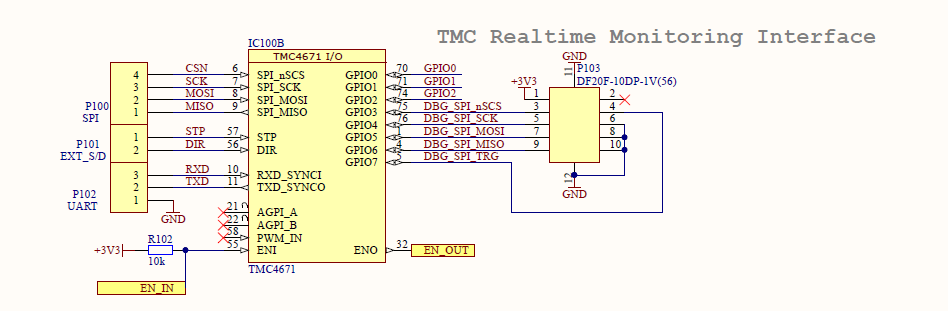
\includegraphics[width=\textwidth]{graphics/TMC4671_SPI_BOB_Schematic}
	\caption{SPI-Input des TMC4671-BOB.}
	\label{fig:Schema_SPI_FOC_Treiber}
\end{figure} 

\newpage

\subparagraph{Ströme Input (ADC)}

Der Eingang zur Strommessung ist mit einem Tiefpass geschützt. Dieser hat die Zeitkonstante:

\begin{equation}
\tau = R308 \cdot C300 = 100\Omega \cdot 100pF = 10ns
\end{equation}

\begin{figure}[h!]
	\centering
	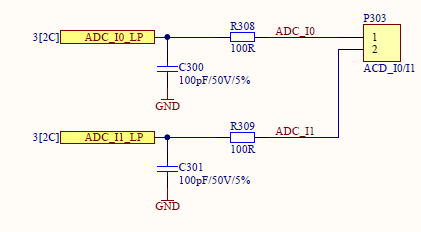
\includegraphics[width=0.5\textwidth]{graphics/TMC4671_Phasenstroeme_BOB_Schematic}
	\caption{Phasenstroeme-Input des TMC4671-BOB.}
	\label{fig:Schema_Phasenstroeme_FOC_Treiber}
\end{figure} 

\subparagraph{Encoder Input (ENC)}

Der Encoder-Input ist ziemlich clever aufgebaut. Um Überspannungen zu verhindern, wird ein Schmitt-Trigger mit eingebautem Level-Shifter verwendet. Der Level-Shifter verhindert dabei ein Anstieg der Eingangsspannung über dessen Eingangsspannung.
Zudem wird mit dem Widerstandsnetzwerk ein entprellen der Encoder-Signale erreicht. Wird der Input auf 0V gezogen, so entlädt sich der Kondensator über die Widerstände R200-R202 mit der Zeitkonstante:

\begin{equation}
\tau = R200 \cdot C204 = 1k\Omega \cdot 100pF = 100ns
\end{equation}

Fällt die Spannung über dem Kondensator während dem Entladen under einen bestimmten Wert, so wird auch der Schmitt-Trigger aktiv und springt auf 0V. Sobald der Eingang nicht mehr vom Encoder auf 0V gezogen wird, so lädt sich der Kondensator über die Widerstände R200-R202 sowie R206,R208,R210. Somit ergibt sich eine längere Zeitkonstante:

\begin{equation}
\tau = (R200 + R210) \cdot C204 = (1k\Omega + 4.7k\Omega) \cdot 100pF = 570ns
\end{equation}

Jetzt geht es bedeutend länger, bis der Kondensator wieder geladen wird. Sobald die Spannung wieder einen bestimmten Wert erreicht, wird der Schmitt-Trigger aktiv und springt auf Versorgungsspannung (3.3V).

\begin{figure}[h!]
	\centering
	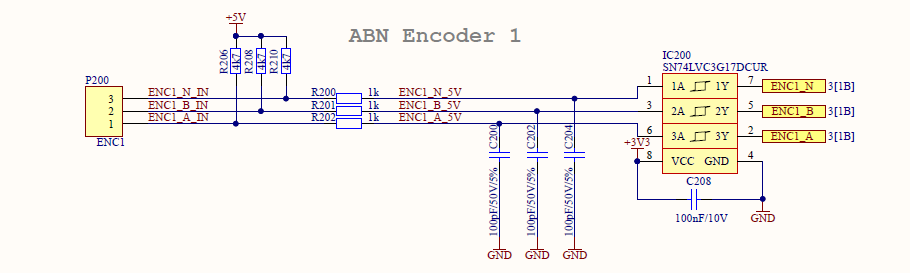
\includegraphics[width=0.7\textwidth]{graphics/TMC4671_ABN_Encoder_BOB_Schematic}
	\caption{ABN-Encoder-Input des TMC4671-BOB.}
	\label{fig:Schema_ABN_Encoder_FOC_Treiber}
\end{figure} 

\subparagraph{Motorspannung Input (48V)}

Die Motorspannung ist wichtig, um einen Kommuntierungsvorgang zu berechnen. Wichtiger als die Zeitkonstante ist hier ein Spannungsteiler, welcher die Motorspannung auf unter 3.3V bringt. Dazu wird folgende Formel angewendet:

\begin{equation}
U_{TMC} = U_M \cdot \frac{R310}{R310 + R311} = 48V \cdot \frac{1k\Omega}{1k\Omega + 100k\Omega} = 0.7V
\end{equation}

\begin{figure}[h!]
	\centering
	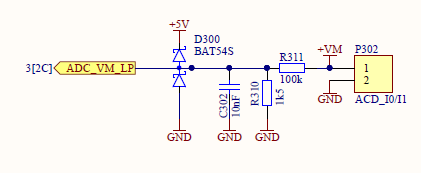
\includegraphics[width=0.7\textwidth]{graphics/TMC4671_Motorspannung_BOB_Schematic}
	\caption{Motorspannung-Input des TMC4671-BOB.}
	\label{fig:Schema_Motorspannung_FOC_Treiber}
\end{figure} 

\subparagraph{Steuersignale Output (PWM)}

Die Ausgangssignale für den Gate-Treiber gehen direkt auf die Header-Pins des MC4671-BOB. Sie werden nicht geschützt.

\begin{figure}[h!]
	\centering
	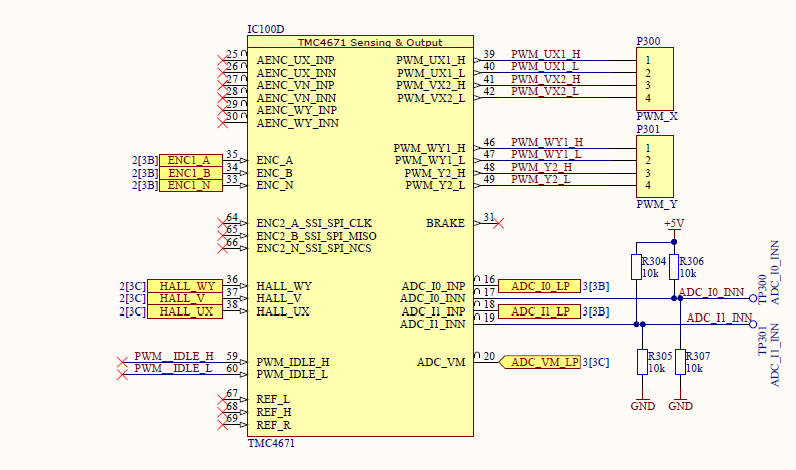
\includegraphics[width=0.7\textwidth]{graphics/TMC4671_PWM_BOB_Schematic}
	\caption{PWM-Output des TMC4671-BOB.}
	\label{fig:Schema_PWM_FOC_Treiber}
\end{figure} 

%\subsubsection{Encoder-Input}\label{subsubsec:Encoder_Input}
%
%Vor einem Analogeingang wird das Signal in der Regel mit einem Tiefpass gefiltert, um stochastische Abweichungen zu verhindern. Dafür werden die Widerstände \textbf{R700-R702} und die Kondensatoren \textbf{C700-C702} verwendet. Die Beschaltung und Dimensionierung wurde aus dem Datenblatt des TMC4671-EVAL-Board entnommen. Die Zeitkonstante des Filters beträgt gemäss Formel \ref{equ:Berechnung_Encoder_LP} 10ns. Das Schaltungsprinzip ist in Abbildung \ref{fig:Schema_Encoder_LP} dargestellt. 
%\begin{equation}
%\tau = R \cdot C = 100\Omega \cdot 100\cdot10^{-12}F = 10 \cdot 10^{-9}s = 10ns
%\label{equ:Berechnung_Encoder_LP}
%\end{equation}
%
%Der Motor hat eine Drehzahl von max. 1500rpm, dies entspricht einer maximalen Periodendauer von $\mathrm{666.\overline{6} \mu}$s. Das Eingangssignal wird deshalb nicht herausgefiltert.
%
%Die Komponenten \textbf{D700-D702} sind Bauteile, welche zwei Shottky-Dioden verbaut haben und sind dazu da, eventuell auftretende Über-/ und Unterspannungen zu verhindern. Abbildung \ref{fig:Schema_Encoder_2_LP} zeigt die Anordnung der internen Dioden an Stelle des
%verwendeten Bauteils. Jede Diode hat eine Durchlassspannung von 0.3V. Liegt in Abbildung \ref{fig:Schema_Encoder_2_LP} beim Eingangssignal eine Spannung von über 5.3V an, wird die Diode an 5V leitend und verhindert ein weiteres Ansteigen der Eingangsspannung. Das Selbe bei Unterspannung, sobald eine Spannung von -0.3V anliegt, wird die Diode an 0V leitend, und verhindert ein weiteres Absinken der Spannung.

%\begin{figure}[h!]
%	\centering	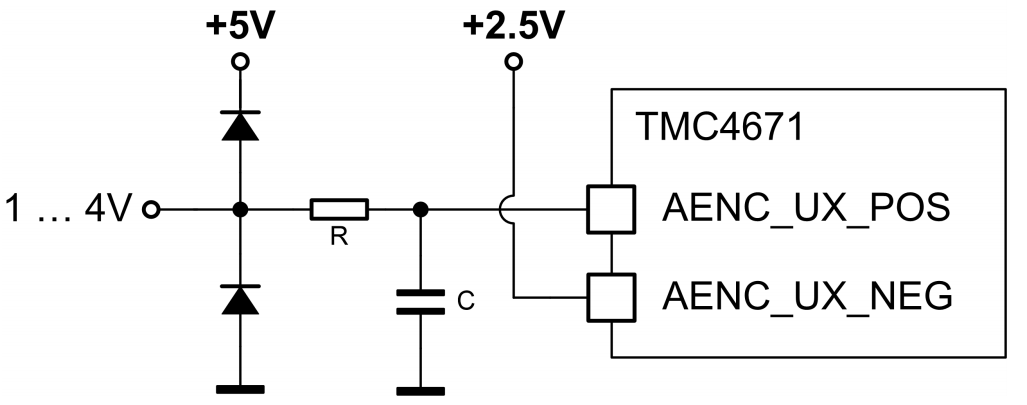
\includegraphics[width=0.5\textwidth]{graphics/Schema_Encoder_2_LP.png}
%	\caption{Teilschema aus Datenblatt TMC4671. Hier mit Shottky-Dioden anstelle IC.}
%	\label{fig:Schema_Encoder_2_LP}
%\end{figure}

%Die Widerstände \textbf{R703-R708} Stellen Spannungsteiler dar, welche gemäss Datenblatt eine benötigte Spannung von 2.5V bereitstellen.
%
%Der Kondensator \textbf{C703} ist ein Stützkondensator und dient der Speisung eines Ecoders. Die Versorgungsspannung wird jedoch nicht für den Resolver benötigt.
%
%Der Header \textbf{J6} ermöglicht, den Resolver an das PCB anzuschliessen.
%
%Abbildung \ref{fig:Schema_Encoder_LP} zeigt das Gesamte Schema mit den Komponenten, welche ein korrektes Einlesen des Resolvers ermöglichen.

%\begin{figure}[h!]
%	\centering	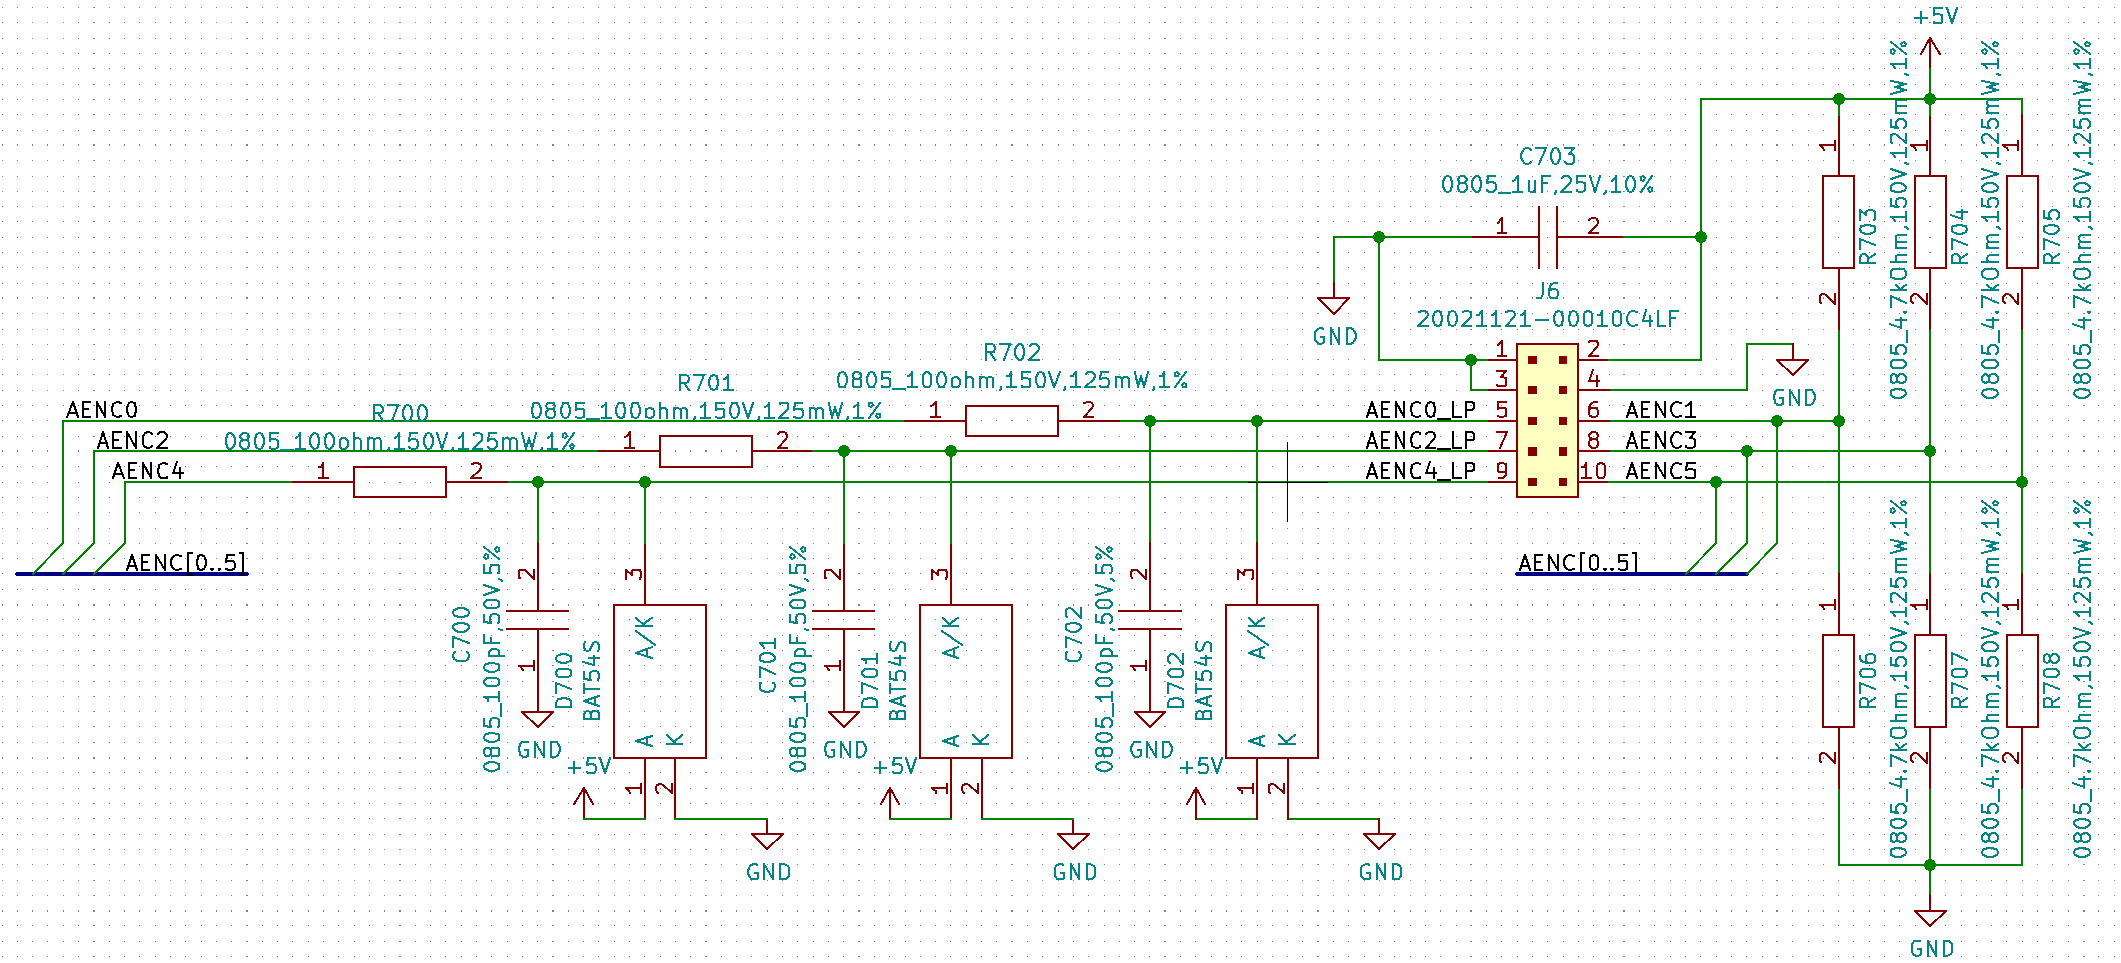
\includegraphics[width=\textwidth]{graphics/Schema_Encoder_LP.png}
%	\caption{Teilschema TMC4671. Hier Input Encoder.}
%	\label{fig:Schema_Encoder_LP}
%\end{figure}

%\subsubsection{Analog-Inputs}\label{subsubsec:Analog_Inputs}
%
%Auch hier wird das Eingangssignal mit einem Tiefpass gefiltert. Dafür werden die Widerstände R711 und R713 sowie die Kondensatoren C707 und C709 verwendet. Die Beschaltung und Dimensionierung wurde aus dem Datenblatt des TMC4671-EVAL-Board entnommen. Die Zeitkonstante des Filters beträgt gemäss Formel \ref{equ:Berechnung_Analog_LP} 400ns. Das Schaltungsprinzip ist in Abbildung \ref{fig:Schema_Analog_LP} dargestellt. \cite[PDF S.25]{trinamic_drawings_2018}
%\begin{equation}
%\tau = R \cdot C = 4\cdot 10^{3}\Omega \cdot 100\cdot10^{-12}F = 10 \cdot 10^{-9}s = 400ns
%\label{equ:Berechnung_Analog_LP}
%\end{equation}
%
%Weiter befindet sich ein zweiter Widerstand in jeder Schaltung
%\todo{Funktion zweiter Widerstand herausfinden.}
%
%Das letzte Bauteil, welches noch beschrieben werden muss, sind die Dioden D703 und D704. Diese stellen jeweils wieder einen Über- bzw. Unterspannungsschutz dar, um den Messeingang des TMC4671 zu schützen. Das Bauteil ist das selbe wie oben im Encoder-Teil, weshalb hier auf eine tiefere Beschreibung verzichtet wird.
%
%\begin{figure}[h!]
%	\centering	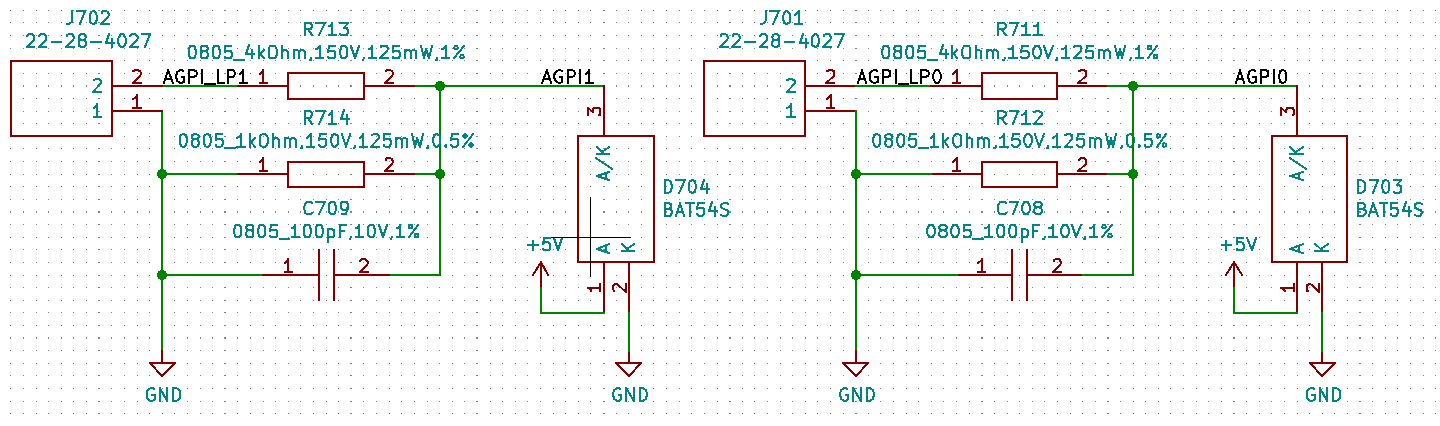
\includegraphics[width=0.8\textwidth]{graphics/Schema_Analog_Inputs_LP.png}
%	\caption{Teilschema TMC4671. Hier Inputs Analog.}
%	\label{fig:Schema_Analog_LP}
%\end{figure}
%
%
%\subsubsection{Motorspannung-Input}\label{subsubsec:Motorspannung_Input}
%
%\cite[PDF S.25]{trinamic_drawings_2018}
%\begin{figure}[h!]
%	\centering	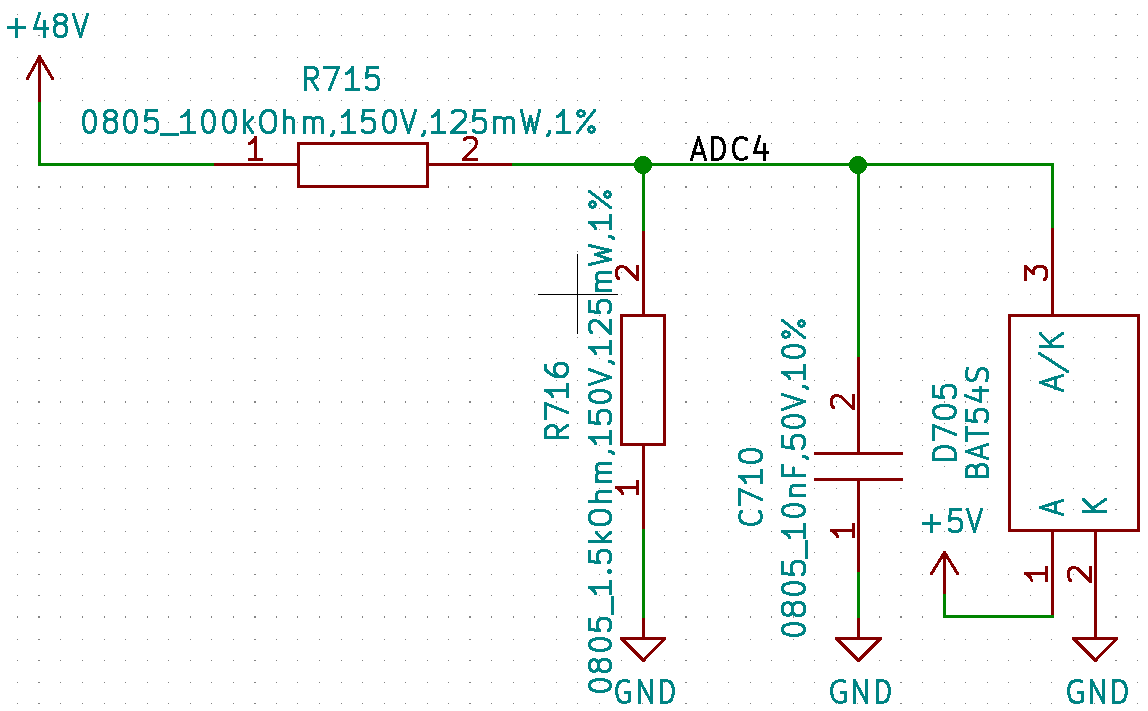
\includegraphics[width=0.45\textwidth]{graphics/Schema_VM_Input_LP.png}
%	\caption{Teilschema TMC4671. Hier Input Motorspannung.}
%	\label{fig:Schema_Encoder_LP}
%\end{figure}

\subsubsection{Gate-Treiber}
\label{subsubsec:Gate-Treiber}

%Nebst dem TMC4671, welcher für die Ansteuerung benötigt wird, braucht es für die Magnetisierung der Spulen des BLDC-Motors eine Schaltlogik. Dabei Handelt es sich um den TMC6200. Dieser ist eine umfangreiche Ergänzung zum TMC4671. Auf den TMC6200 und weitere benötigte Komponenten wird im folgenden eingegangen.
%\subsubsection{Problem}\label{subsubsec:Problem_TMC6200}

Der Motor wird über eine H-Brücke gesteuert. Dies bedingt pro Spule zwei MOSFET's, um diese entsprechend magnetisieren zu können. Um einen MOSFET in einen leitenden Zustand zu bringen, muss das Gate des MOSFET's mit einer elektrischen Ladung gefüllt werden. Während diesem Vorgang hat am Gate ein kapazitives Verhalten, was bedeutet, dass bei jedem Schaltvorgang Ströme fliessen. Um ein optimales Schaltverhalten zu erreichen, die Umschaltverluste zu verringern und somit die daraus entstehende Abwärme zu verhindern, ist es vorteilhaft die Gates so schnell wie möglich laden und entladen zu können. Da kommt der Gate-Treiber ins Spiel. Dieser ladet und entladet das Gate schnell genug und stellt die dazu benötigte Energie für das Gate zur Verfügung.

\paragraph{Schema}\mbox{}\\

Damit ein Aufbau mit mehreren Gate-Treibern vermieden werden kann und einige Zusatzfunktionen wie Strommessung, Messverstärkung, Kurzschlussdetektion etc. genutzt werden können, wurde während des Entwicklungsprozesses ein Gate-Treiber von Trinamic ausgewählt. Das entsprechende Bauteil ist der TMC6200. Das Blockdiagramm und eine Beispielschaltung befinden sich im Anhang Kapitel \ref{Appendix:Schaltung_TMC6200} und \ref{Appendix:Blockdiagramm_TMC6200}. Das Blockdiagramm zeigt, dass der TMC6200 aus einer Treiber-Logik für den Motor, einem SPI-/Pinsettings-Interface, einer Diagnosenlogik, Strommessschaltung und diversen unterstützenden Schaltungen wie Spannungsversogrung besteht. Das Schema ist in Abbildung \ref{fig:Schema_Gate_Treiber} zu sehen.


\begin{figure}[H]
	\centering
	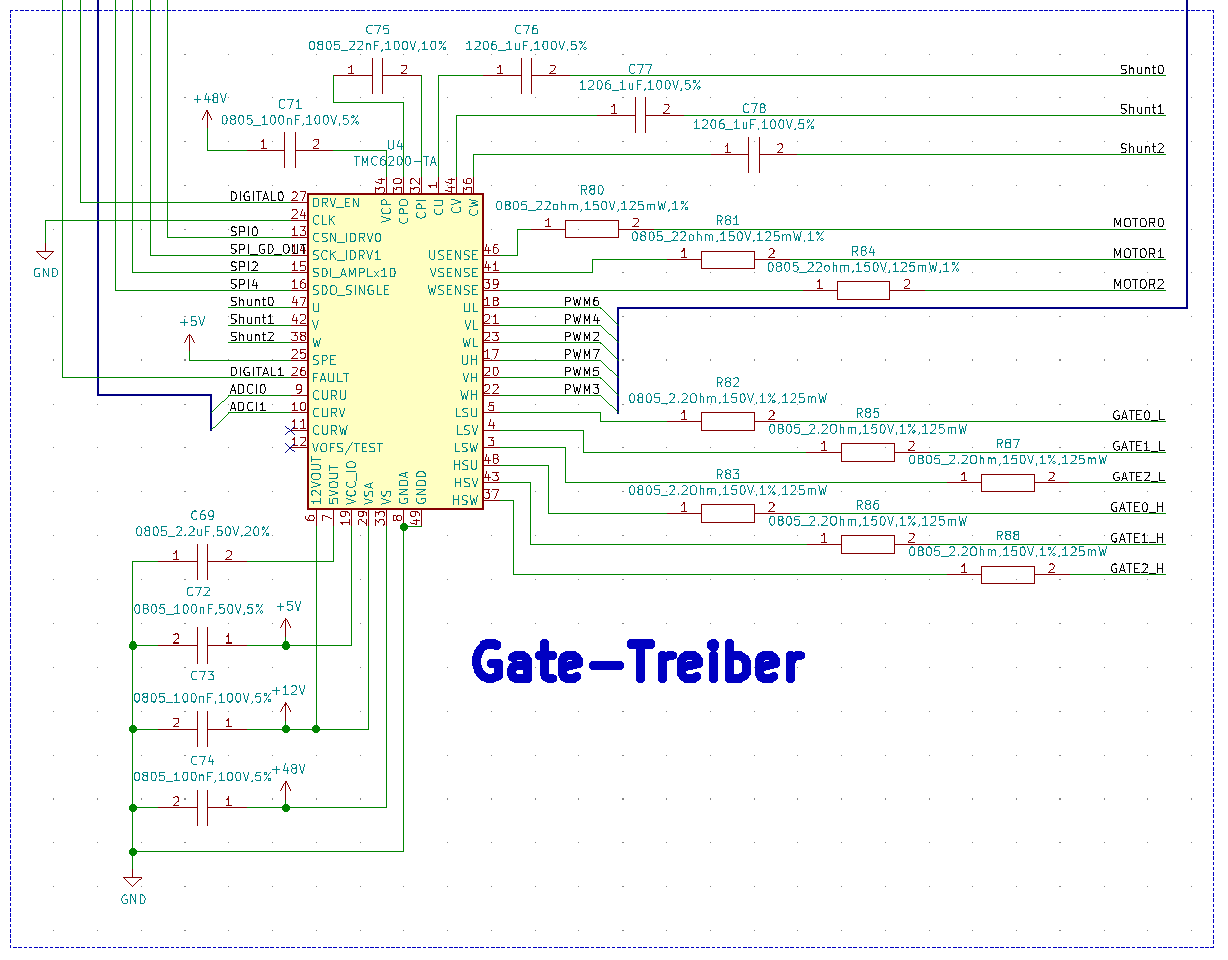
\includegraphics[width=\textwidth]{graphics/Schema_Gate_Treiber}
	\caption{Schema Gate-Treiber.}
	\label{fig:Schema_Gate_Treiber}
\end{figure}

%\begin{figure}[h!]
%	\centering
%	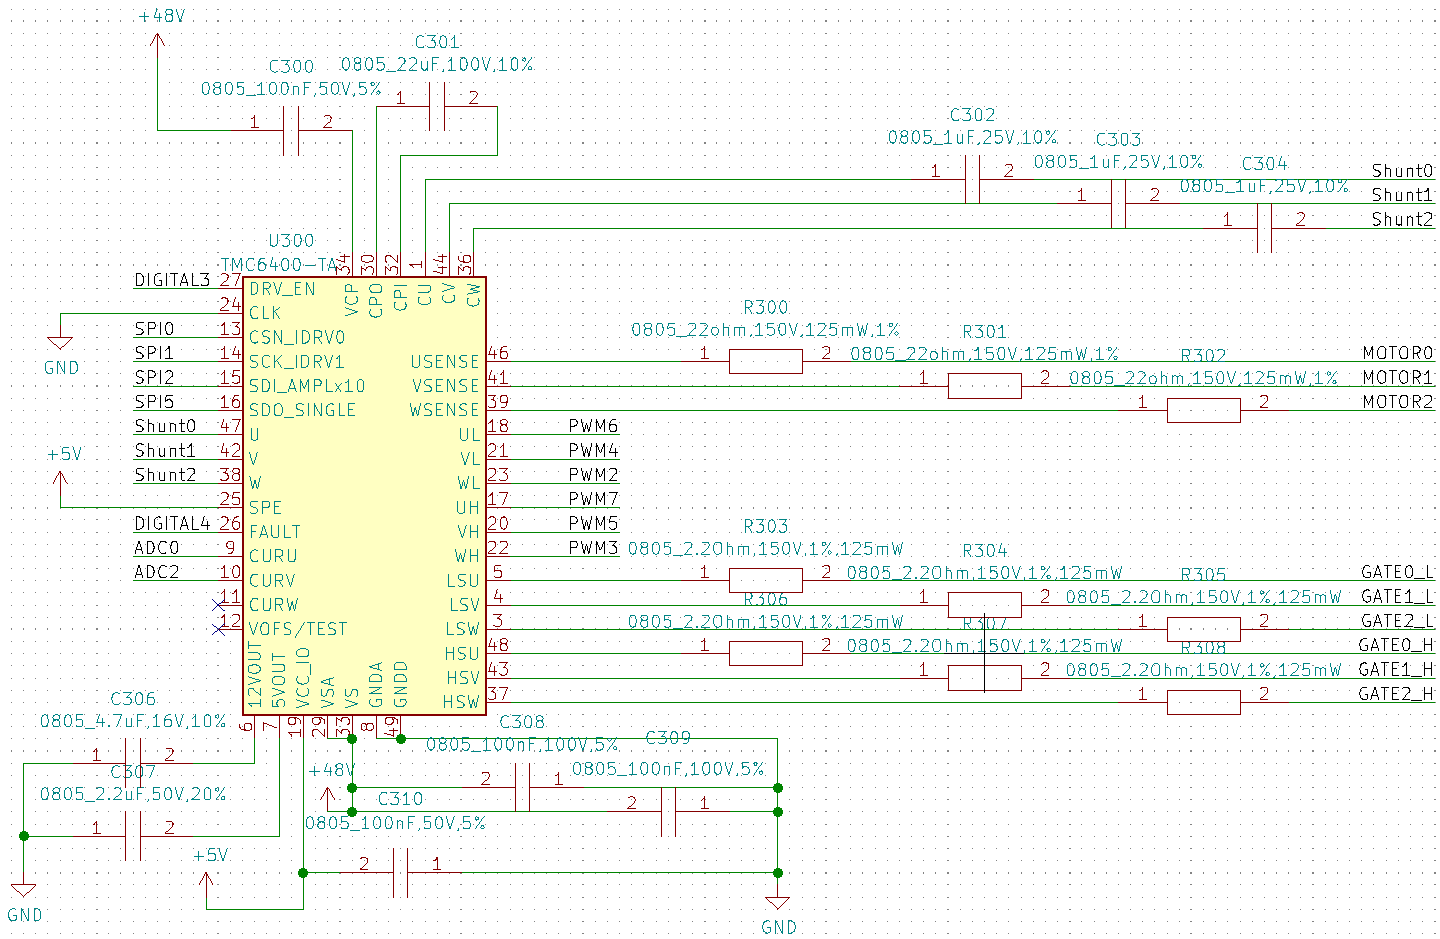
\includegraphics[width=0.8\textwidth]{graphics/TMC6200_Schema.png}
%	\caption{Teilschema Ansteuerung Motor. Hier Gate-Treiber-IC TMC6200.}
%	\label{fig:Schema_TMC6200}
%\end{figure}
%\begin{figure}[h!]
%	\centering
%	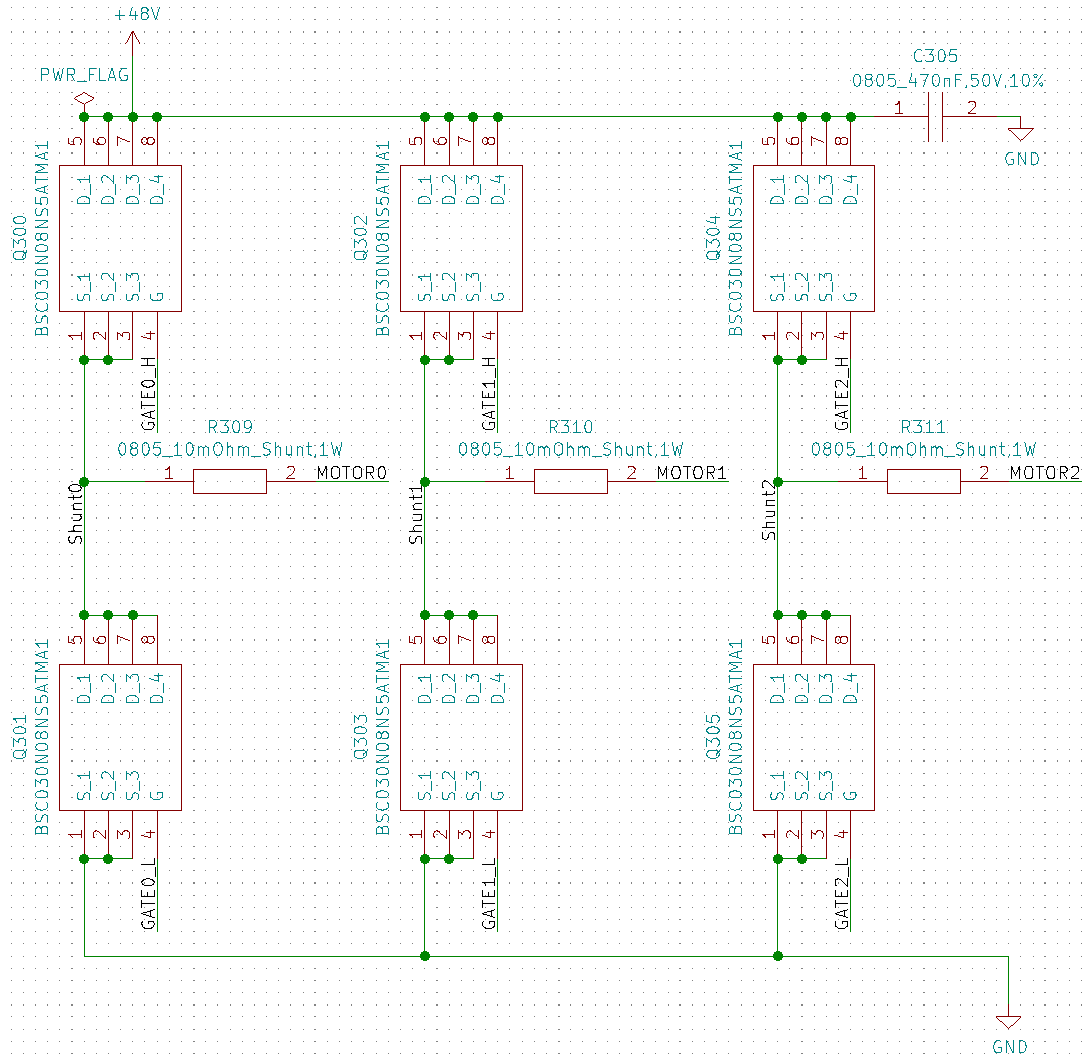
\includegraphics[width=0.6\textwidth]{graphics/H_Bruecke_Schema.png}
%	\caption{Teilschema Ansteuerung Motor. Hier H-Brücke.}
%	\label{fig:Schema_TMC6200}
%\end{figure}

\paragraph{Funktionsbeschrieb der Schaltung}\mbox{}\\

%\subparagraph{Shunt-Widerstände $\mathrm{\mathbf{R_{Sense}}}$}
Für die Messung des Stromes wird ein Shunt in Serie mit der Spule des BLDC-Motors geschaltet. Die Shunts R89 - R91 sind in Abbildung \ref{fig:Schema_H_Bruecke_und_BLDC} zu sehen. Durch den fliessenden Strom liegt eine Spannung über dem Shunt, welche dann vom TMC6200 verstärkt wird und aufbereitet an den Kontroll-Chip TMC4671 ausgegeben wird. Die Verstärkung sowie Offset auf das Signal sind über SPI programmierbar.
Die Dimensionierung der Widerstände und die darauf folgende Programmierung des TMC6200 sind schon von Trinamic ermittelt worden. Es wird empfohlen, die Widerstände nach dem Maximalstrom des Motors auszuwählen. Im Falle des AKM22h sind dies 5A. Darüber hinaus wird empfohlen, eine Überdimensionierung von 25-50\% vorzunehmen. Die Schaltung für den PartyMixer wird auf 10A ausgelegt. Eine von Trinamic erstellte Tabelle  empfiehlt einen Widerstand von 10m\textOmega\ für die Shunt-Widerstände und einen Verstärkungsfaktor der Phasenströme von 10. Die Tabelle ist im Anhang Kapitel \ref{Appendix:Shunt} zu finden. \cite[S.31]{trinamicmotion_control_gmbh__co_kg_tmc6200_2019}

%\begin{tabular}{lll}
%$\mathbf{R_{Sense}}$ =  \textbf{10m\textOmega}\\
%\textbf{Verstärkungsfaktor}= \textbf{10x}   
%\end{tabular}

%\paragraph{Gate Vorwiderstände $\mathrm{\mathbf{R_{Gate}}}$}

Da das Gate ein kapazitives Verhalten zeigt, ist der Strom, welcher zu Beginn ins Gate fliesst, sehr hoch. Der Gate-Vorwiderstand begrenzt diesen, um das Gate und den Pin des TMC6200 vor Überströmen zu schützen. Die Vorwiderstände R82 - R83 und R85 - R88 sind in Abbildung \ref{fig:Schema_Gate_Treiber} zu sehen.
Die Dimensionierung der Gate-Widerständen wurde an die MOSFET Gate-Drain-Ladung (Miller charge) angelehnt. Auch in diesem Falle wurden von Trinamic schon einige Parameter ermittelt und im Anhang \ref{Appendix:Gate_Vorwiderstand} dargestellt. Die Gate-Ladung des ausgewählten MOSFET's beträgt 61nC. Aus der Tabelle kann somit ausgelesen werden, dass der Vorwiderstand R$_{Gate}\leq$2.5\textOmega\ sein sollte und das programmierbare Register DRV\_STRENGTH auf 1 bis 3 gesetzt wird. \cite[S.13]{trinamicmotion_control_gmbh__co_kg_tmc6200_2019}

%\begin{tabular}{lll}
%$\mathrm{\mathbf{R_{Gate}}}$ & \textbf{=} & $\mathrm{\mathbf{R_{Gate}\leq2.5\Omega}}$ \\
%\textbf{DRV\_STRENGTH} & \textbf{=} & \textbf{1 bis 3}
%\end{tabular}

%\paragraph{Schutzwiderstände Messeingang $\mathrm{\mathbf{R_{Protect}}}$}

Wird von einem High-Zustand in einen Low-Zustand gewechselt, kann aufgrund von Induktivitäten der Shunts oder deren Verbindungen die Spannung unterschiessen. Der Schutzwiderstand schützt den Messeingang des TMC6200 vor diesem Effekt. Die Schutzwiderstände R80, R81 und R84 sind in Abbildung \ref{fig:Schema_Gate_Treiber} zu finden.
Die Dimensionierung dieses Widerstands wird im Datenblatt mit einem Widerstandswert zwischen 10\textOmega\ und 22\textOmega\ angegeben.\cite[S.10]{trinamicmotion_control_gmbh__co_kg_tmc6200_2019}

%\begin{tabular}{lll}
%$\mathrm{\mathbf{R_{P}}}$ & \textbf{=} & \textbf{10\textOmega\ bis 22\textOmega}\\
%\end{tabular}

%\paragraph{Bootstrap Kondensatoren $\mathrm{\mathbf{C_{Bootstrap}}}$}

Die Bootstrap-Kondensatoren werden benutzt, um die Gate-Spannung am High-Side-MOSFET auf die Schaltspannung (48V) plus die Gatespannung anzuheben. Die Kondensatoren C76 - C78 in Abb. \ref{fig:Schema_Gate_Treiber} unterstützen diesen Effekt.
Die Dimensionierung dieser Kondensatoren wird im Datenblatt mit einem Kapazitätswert zwischen 470nF und 1\textmugreek F angegeben, bei einer Nennspannung von 16V oder 25V. Weiter gilt gemäss Datenblatt, dass bei MOSFET's mit einem $\mathrm{Q_G \geq 40nC}$ die Gatekapazität 1\textmugreek F sein soll. Da die Kapazität 61nF beträgt, ist dies der Fall. Die Bootstrap-Kondensatoren werden deswegen mit 1\textmugreek F dimensioniert. \cite[S.10]{trinamicmotion_control_gmbh__co_kg_tmc6200_2019}

%\begin{tabular}{lll}
%$\mathrm{\mathbf{C_{Bootstrap}}}$ & \textbf{=} & \textbf{1\textmugreek F (25V)}\\
%\end{tabular}

%\paragraph{Externer Gate-Spannungsregler}

Aufgrund der hohen Versorgungsspannug (48V), treten im IC über den Gate- und 5V- Spannungsreglern erhebliche Verluste auf. Um diese Verluste zu reduzieren, wird gemäss Datenblatt \cite[S.11]{trinamicmotion_control_gmbh__co_kg_tmc6200_2019} geraten, eine externe Gate-Spannung anzuhängen. Für beste Resultate wird eine Spannung von 12V $\pm$ 1V empfohlen.
Die Dimensionierung der benötigten Kondensatoren ist im Anhang Kapitel \ref{Appendix:Gate_Spannungsversorgung} zu finden. Für den Kondensator C69 sollten 2.2\textmugreek F verwendet werden und für den Kondensator C73 100nF.

%\begin{tabular}{lll}
%$\mathrm{\mathbf{C_{69}}}$ & \textbf{=} & \textbf{2.2\textmugreek F}\\
%$\mathrm{\mathbf{C_{73}}}$ & \textbf{=} & \textbf{100nF}\\
%\end{tabular}

\subsection{Flüssigkeitsbeförderung}
\label{subsec:Flüssigkeitsbeförderung}

Für die Flüssigkeitsbeförderung sind zwei essentielle Komponenten  erforderlich. Einerseits muss die Flüssigkeit befördert werden, anderseits muss diese auch dosierbar sein. Diese zwei Hauptaufgaben übernehmen die Pumpen und die Durchflussmessgeräte. 



\subsubsection{Pumpen}
\label{subsubsec:Pumpen}



\subsubsection{Durchflussmessgeräte}
\label{subsubsec:Durchflussmessgeräte}

Um die Flüssigkeiten wie gewünscht abfüllen zu können, müssen diese sauber dosiert werden können. Zu diesem Zweck wurden Durchflussmessgeräte eingesetzt. Bei diesen Durchflüssmessgeräten handelt es sich um volumetrische Durchflussmessgeräte von Sea, welche bei Durchfluss eine Pulsfolge ausgeben. Diese können dann mittels Elektronik ausgewertet werden. \cite{five__tools_store_us_nodate}

\paragraph{Schema}\mbox{}

Das Schema für diese Schaltung ist in Abbildung \ref{fig:Schema_Durchflussmessgeräte} zu sehen. Es beinhaltet lediglich einen \todo{Stütz/Filterkondensator?}Filterkondensator an der Speisung und einen Stecker, an welchem die Durchflussmessgeräte angeschlossen werden können.

\begin{figure}[h!]
	\centering
	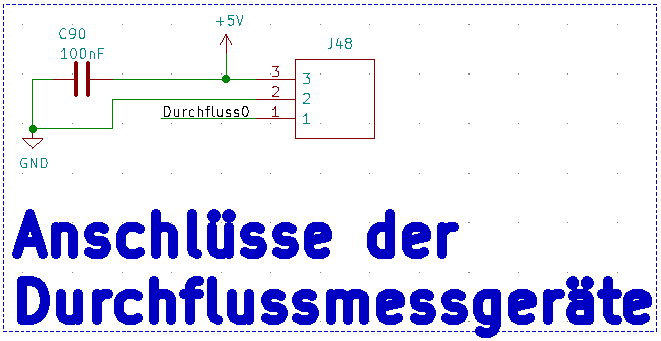
\includegraphics[width=0.6\textwidth]{graphics/Schema_Durchflussmessgeraete.png}
	\caption{Schema der Durchflussmessgeräte.}
	\label{fig:Schema_Durchflussmessgeräte}
\end{figure}

\paragraph{Funktionsbeschrieb der Schaltung}\mbox{}

Die Durchflussmessgeräte haben drei Anschlüsse. Zum einen ist dies ein Speisungseingang von 5V und eine Groundleitung. Der dritte Pin der Durchflussmessgeräte ist ein Signalpin, welcher bei Durchfluss ein gepulstes Signal mit 5V und 50\% Duty-Cycle ausgibt. Da dieses Signal direkt vom Mikrocontroller ausgewertet werden kann, ist keine weitere Elektronik erforderlich. Zur Auswertung der Signale werden gemäss Kapitel \ref{subsec:Mikrocontroller} wiederum Digitalpins als Eingänge verwendet. \cite{five__tools_store_us_nodate}  

\clearpage
\subsection{Programmierschnittstellen}
\label{subsec:Programmierschnittstellen}

Die beiden Devices, welche programmiert werden müssen, werden über die USB-Schnittstelle programmiert. Im Folgenden ist in Abbildung \ref{fig:Schema_USB_B} nur das Schema des Flash-Interfaces für das ESP32 ersichtlich. Es unterscheidet sich zum Flash-Interface des ATMega2560 in der Anzahl Steuerleitungen. Auf das Flash-Interface des Atmega2560 wird nicht eingegangen, da die Funktionen die selben sind.

\clearpage
\subsubsection{USB-B}
\label{subsubsec:USB-B}

\begin{figure}[h!]
	\centering
	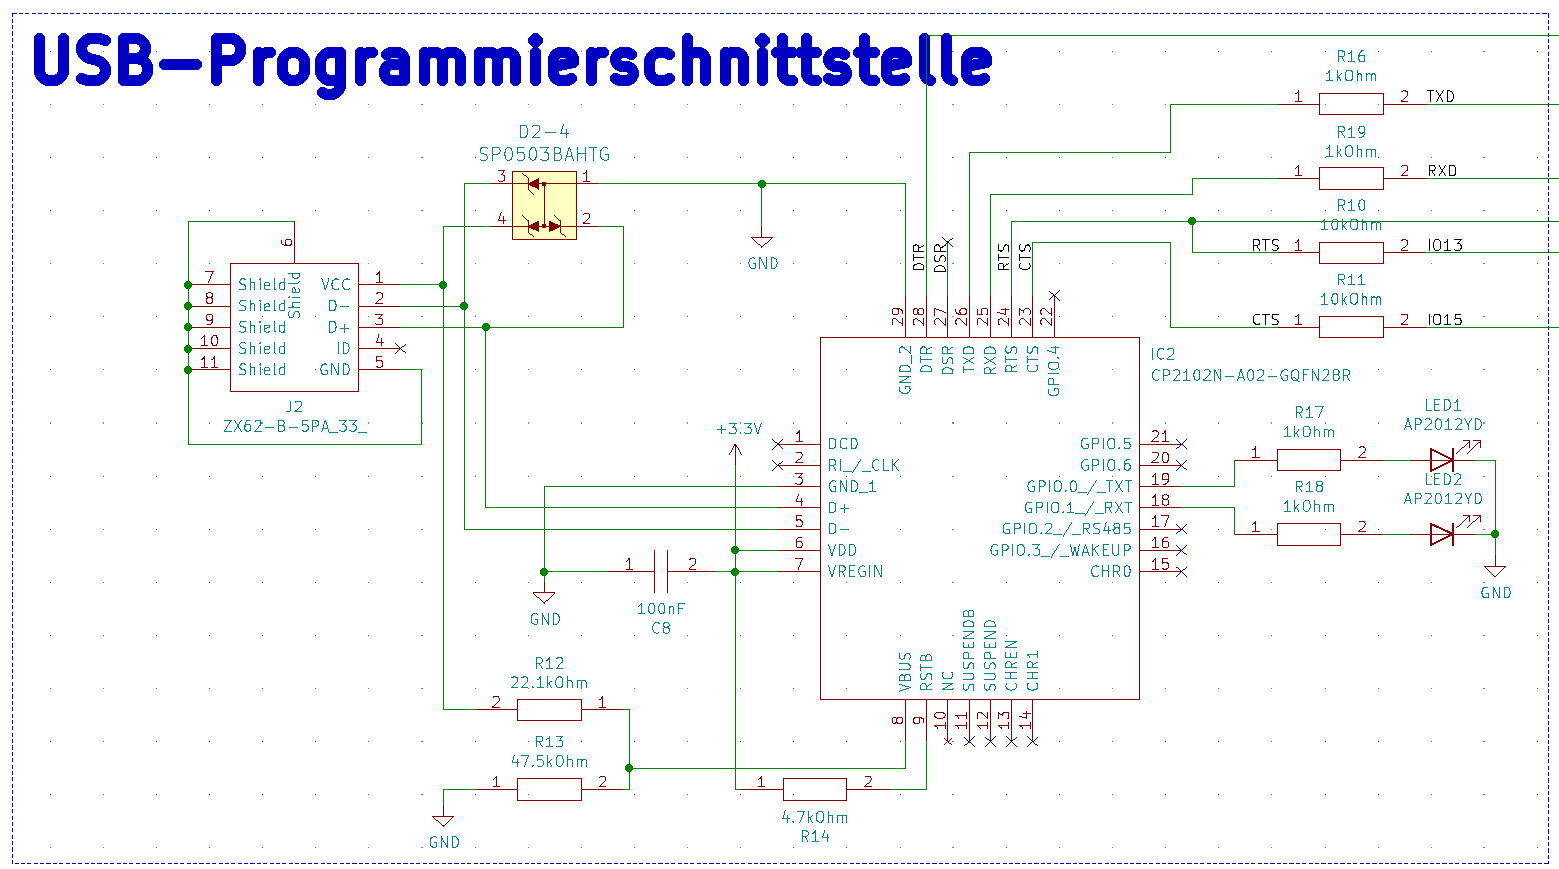
\includegraphics[width=0.5\textwidth]{graphics/Schema_USB_B}
	\caption{Schema USB-B.}
	\label{fig:Schema_USB_B}
\end{figure}



\clearpage
\subsection{Benutzerschnittstellen}
\label{subsec:Benutzerschnittstellen}



\subsubsection{Display}
\label{subsubsec:Display}

Der Benutzer bedient den PartyMixer via dem Nextion Touch-Display. Dabei handelt es sich um das Display NX8048T070. Das GUI basiert dabei auf den Funktionen, die in der Software Nextion Editor zur Verfügung gestellt werden. Die Funktionen umfassen:
\begin{itemize}
\item Erstellen von Seiten, die auf dem Display angezeigt werden.
\item Setzen von Buttons, Slider und Textfeldern auf den Seiten.
\item Speichern von Grafiken, die auf den Seiten angezeigt werden.
\item Kommunizieren über UART um Aktionen auszulösen.
\end{itemize}

\paragraph{Schema}\mbox{}

Um das Display mit der Leiterplatine zu verbinden, braucht es einen Stecker und einen Stützkondensator nahe der Pins am Spannungsausgang, um die Versorgungsspannung zu glätten. Auf eine Abbildung wird verzichtet, der Stecker für das Display ist jedoch im Schema auf Seite 7 zu sehen, welches im Anhang Kapitel \ref{Appendix:Schema_Print} eingefügt ist.

\paragraph{Funktionsbeschrieb der Schaltung}\mbox{}

Die Funktionen werden durch das Stützen der Versorgungsspannung mit dem Kondensator und der Anbindung des Displays an die Leiterplatine gegeben.

\newpage
\subsubsection{ESP}
\label{subsubsec:ESP}

Für die Implementierung des WiFi's wird das ESP32 verwendet. Die Hauptfunktion im Schema ist die Kommunikation mit dem Mikrocontroller über die zweite serielle Schnittstelle. Die Ansteuerung zum Schreiben des Programmspeichers muss so gestaltet werden, dass der Boot-Modus automatisch gestartet werden kann, wenn ein Code hochgeladen werden soll. Dies hat eine zusätzliche Schaltung zur Folge. 

\paragraph{Schema (WiFi-Modul)}\mbox{}

In Abbildung \ref{fig:Schema_ESP32} wird das Schema rund um das ESP32 an sich gezeigt. Es beinhaltet Stütz- und Filterkondensatoren sowie einige Pull-up- und Pull-down-Widerstände, welche verwendet werden, um einen vordefinierten Grundzustand beim Booten des ESP32-Moduls zu erreichen (Strapping-Pins). Weiter gibt es einen Kondensator, welcher dazu da ist, bei gewünschter Zeit in den Boot-Modus zu gelangen. 

\begin{figure}[h!]
	\centering
	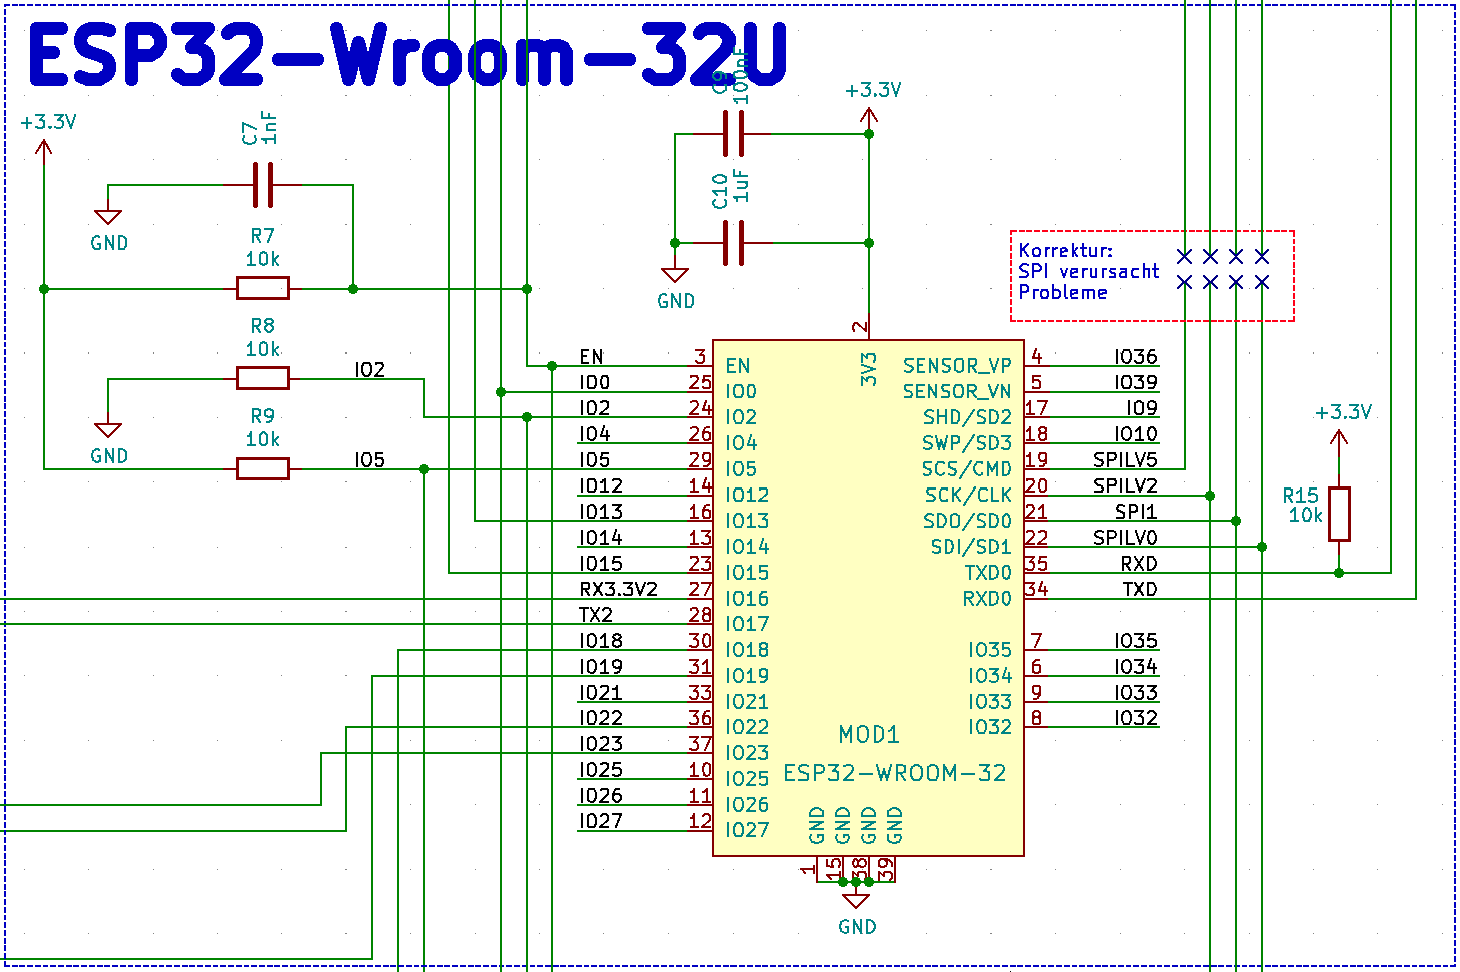
\includegraphics[width=\textwidth]{graphics/Schema_ESP32}
	\caption{Schema ESP32-Wroom-32U.}
	\label{fig:Schema_ESP32}
\end{figure}

\paragraph{Funktionsbeschrieb der Schaltung (WiFi-Modul)}\mbox{}

Das ESP32 ist mit MOD1 beschriftet, es übernimmt die in Kapitel \ref{subsec:Wirelessmodul} beschriebenen Funktionen. Die Kondensatoren C9 und C10 dienen zu Stütz- und Filterzwecken am Spannungseingang.  Über den EN-Pin wird das Modul ein- und ausgeschaltet (acitve high). Der Widerstand R7 ist ein Pull-Up für Chip-Enable. Die Widerstände R8, R9, R10 und R11 sind an die Strapping-Pins angeschlossen. Über diese werden beim Aufstarten des ESP32 der Boot-Modus, die Versorgungsspannung von VDD\_SDIO\footnote{Secure Digital Input Output}-Slave (Erweiterung der SD-Spezifikationen) und andere Initialisierungseinstellungen konfiguriert. Details zu den Konfigurationen sind in Tabelle \ref{tab:Strapping_pins} aufgelistet\footnote{https://www.espressif.com/sites/default/files/documentation/esp32\_datasheet\_en.pdf S.13}. Der Widerstand R15 zieht U0TXD auf HIGH. Aus Tabelle \ref{tab:Einfluss_Pins_auf_Boot_Modus} ist ersichtlich, dass dieser für den normalen Boot-Modus auf HIGH sein muss. Für den Download-Boot-Modus hat dieser kein Einfluss. Mit dem Kondensator C7 wird sichergestellt, dass nach einem Reset der Bootmodus gestartet werden kann. Wird der Reset-Pin au LOW gezogen, so entlädt sich der Kondensator. Sobald der Reset-Pin auf HIGH gezogen wird, dauert es länger, bis ein logic High-Zustand am CMOS-Eingang erkannt wird. Wird der Pin IO0 auf LOW gezogen, bevor der Enable-Pin nach einem Reset einen HIGH-Zustand erreicht, so wird das ESP32 in den Download-Boot-Modus gesetzt. Um automatisch in diesen Boot-Modus zu kommen benötigt es eine Logik, welche im Folgenden erklärt wird.

\paragraph{Schema (Automatische Boot-Logik)}\mbox{}

In Abbildung \ref{fig:Schema_ESP32_Flashbuttons} wird die Schaltung gezeigt, welche verwendet wird, das ESP32-Modul in den gewünschten Boot-Zustand zu bringen. Für die Beschaltung der automatischen Boot-Logik benötigt es eine Schaltung mit DTR und RTS als Inputs vom USB-UART-Converter her und EN und IO0 als Outputs auf das ESP32. Die Buttons können bei Bedarf verwendet werden, sind für den automatischen Boot-Modus jedoch nicht zwingend nötig. Sie könnten dazu verwendet werden, manuell in den Bootmodus zu gelangen.\\
Die Widerstände R20 und R21 sind Vorwiderstände an der Basis der Transistoren Q1 und Q2. R22 und R23 sind Pull-Up-Widerstände für die EN- und IO0-Leitung. Die Kondensatoren C13 und C12 dienen zum entprellen. Die Widerstände R25 und R24 begrenzen den Strom bei Drücken der Buttons S1 und S2.

\begin{figure}[h!]
	\centering
	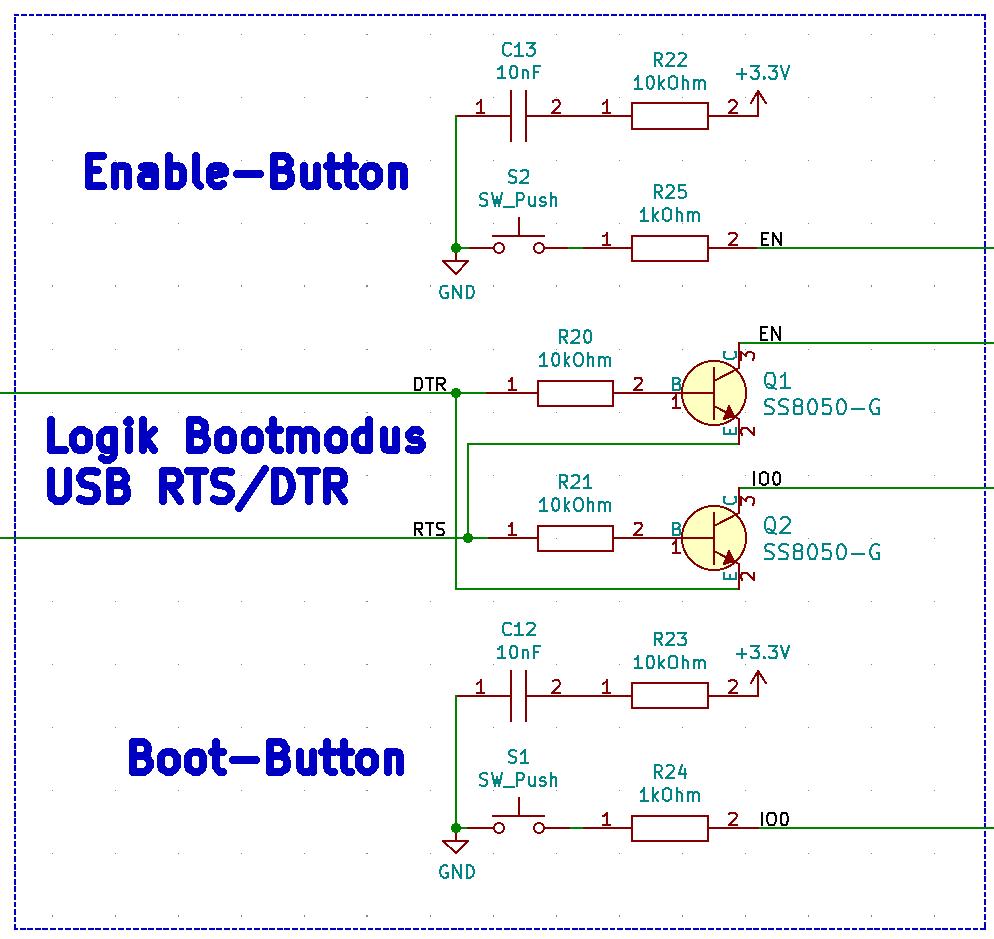
\includegraphics[width=0.7\textwidth]{graphics/Schema_ESP32_Flashbuttons}
	\caption{Schema ESP32-Wroom-32U.}
	\label{fig:Schema_ESP32_Flashbuttons}
\end{figure}

\newpage

\paragraph{Funtionsbeschrieb der Schaltung (Automatische Bootlogik)}\mbox{}



\subsubsection{RFID}
\label{subsubsec:RFID}


\subsection{Beleuchtung}
\label{subsec:Beleuchtung}



\subsection{Mikrocontroller}
\label{subsec:Mikrocontroller}

Der Mikrocontroller ist die Seele, das Gehirn der Maschine. Er muss in der Lage sein mit allen Komponenten auf der Platine zu kommunizieren, die Tasks zu verarbeiten und abhandeln. Der ATMega2560 übernimmt diese Aufgabe.

\paragraph{Schema}\mbox{}

Das Schema besteht aus dem Mikrocontroller IC8 mit den fünf Stützkondensatoren C62, bis C66 an den Spannungseingängen. Mit dem Full Swing Oscillator Crystal Y2 und den Kondensatoren C58 und C59 wird eine Frequenz von 16MHz generiert. Der Reset-Button SW3 dient dazu, den Mikrocontroller manuell neu zu starten. Der dazugehörige Kondensator C81 entprellt den Button und der Widerstand R74 zieht die Leitung mittels Pull-up auf VCC. Mittels dem ISP-Stecker kann über einen Programmer, z.B AVR MKII, auf den Mikrocontroller zugregriffen werden. Der DIP-Switch ist dazu da, die SPI-Leitungen von der ISP-Schnittstelle zu trennen. Die LED D9 gibt Auskunft ob Spannung am Mikrocontroller anliegt.

\begin{figure}[!h]
\center
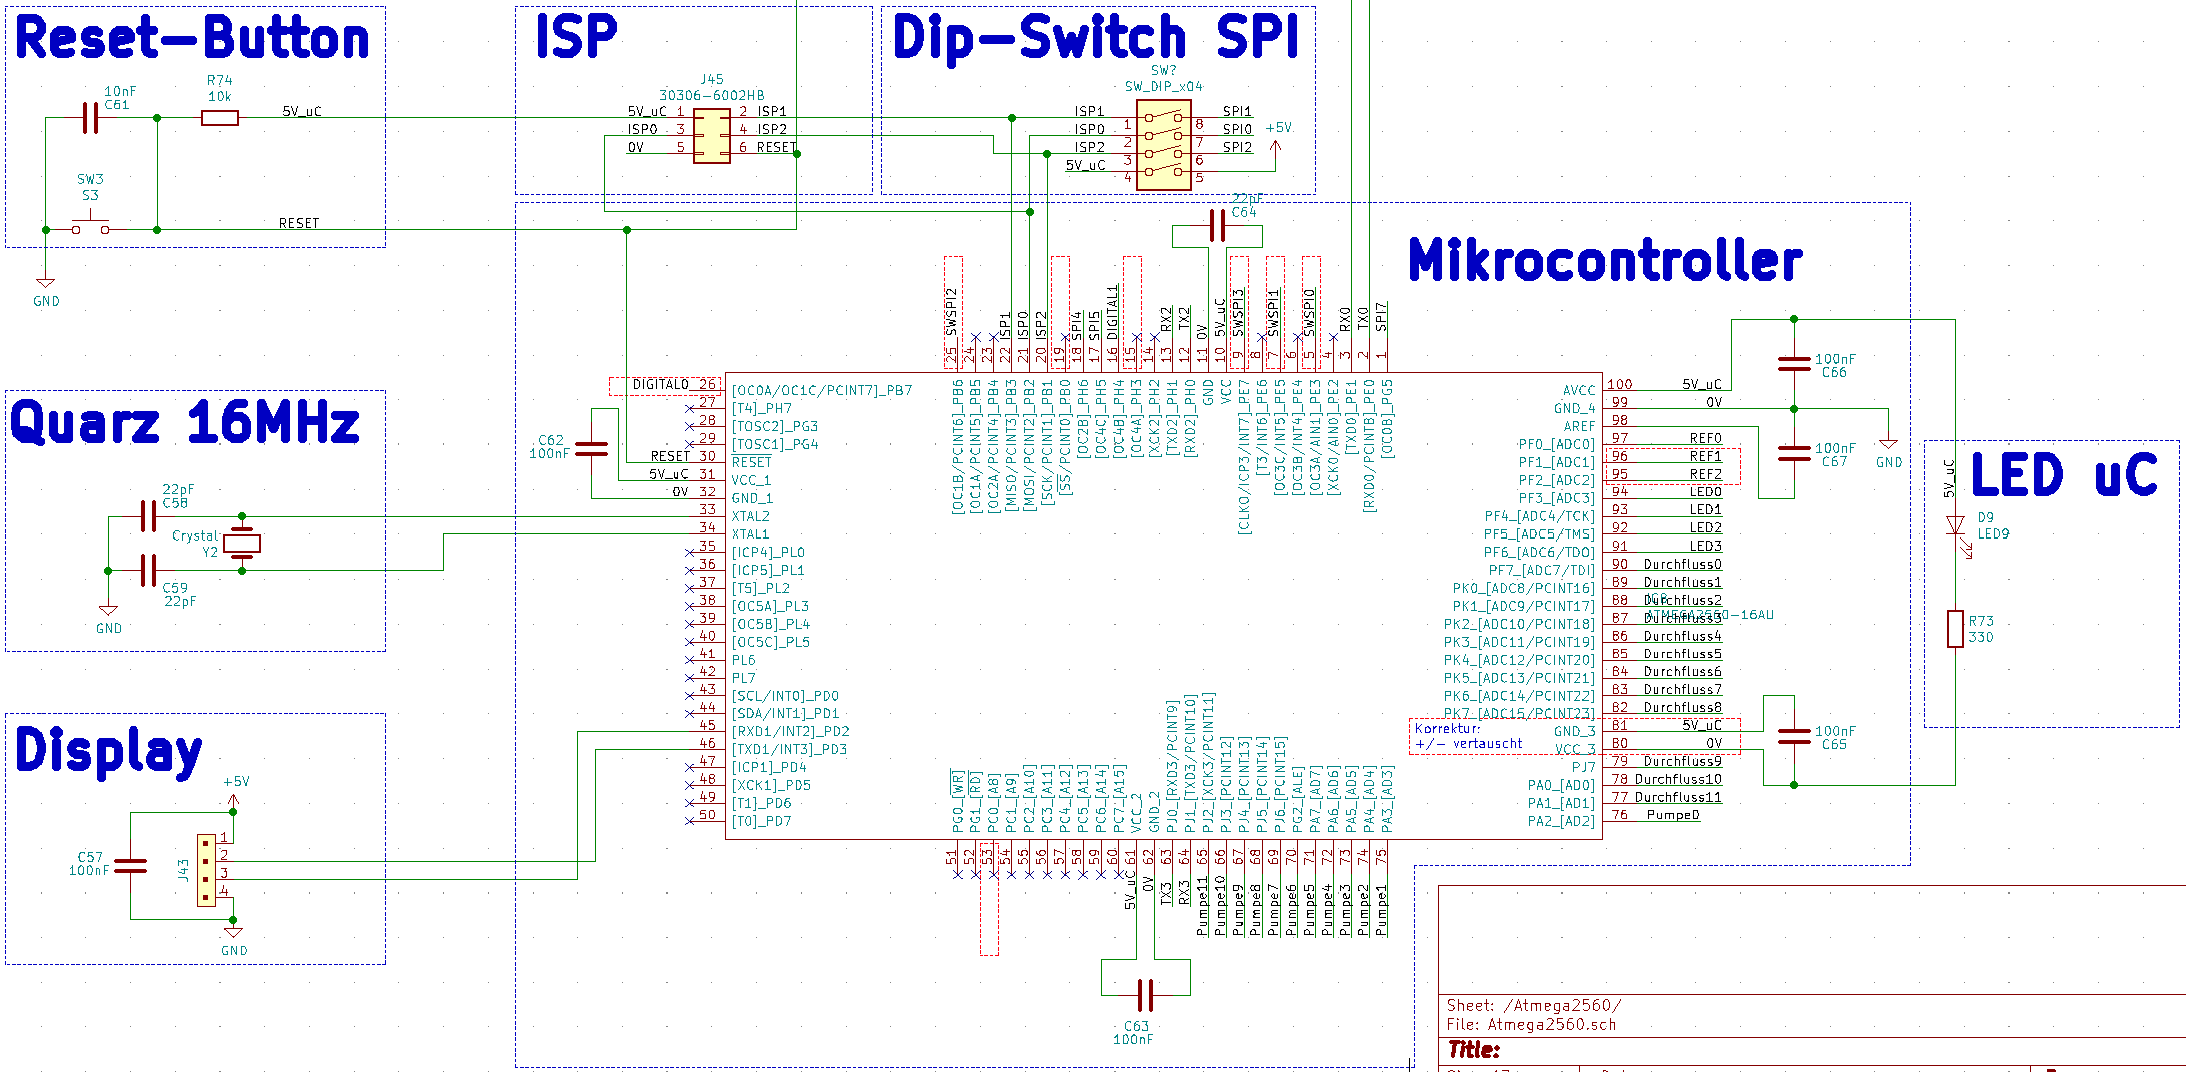
\includegraphics[width = \textwidth]{graphics/Schema_uC}
\caption{Schema Mikrocontroller}
\label{fig:Schema_uC}
\end{figure}

\paragraph{Funktionsbeschrieb der Schaltung}\mbox{}

Die Stüzkondensatoren halten die Spannung am Mikrocontroller konstant. Die Quarz-Schaltung wird gebraucht, da der Mikrocontroller nur eine 8MHz-RC-Clock integriert hat, jedoch mit 16MHz gearbeitet wird. Der Reset-Button zieht in gedrücktem Zustand die Reset-Leitung auf GND. Dabei entlädt sich der Kondensator schnell, da er kurzgeschlossen wird. In offenem Zustand lädt sich der Kondensator über den Widerstand R74 mit einer Zeitkonstante von $\tau = R_{74} \cdot C_{81} = 100us$. Die Trennung von SPI und ISP wird gemacht, sodass gewährleistet ist, dass bei der Inbetriebnahme des Mikrocontrollers die restlichen SPI-kommunikationsfähigen Komponenten nicht mitreden können. Zudem kann die 5V-Versorgungsspannung des Mikrocontroller vom Rest der Platine getrennt werden, sodass dieser auch bei ausgeschalteter Board versorgt werden kann, ohne die anderen Komponenten zu speisen. Deswegen auch die Betriebs-LED.

\subsection{SD-Karte}
\label{subsec:SD-Karte}

Auf der mikroSD-Karte werden die Getränke-, Zutaten, Maschinenfiles abgelegt. Die mikroSD-Karte ist FAT32 formatiert und benötigt ein  mikroSD-Adapter um an das System angeschlossen zu werden.

\paragraph{Schema}\mbox{}

In Abbildung \ref{fig:Schema_SD_Karte} ist das Schema der SD-Karte zu sehen. Darin erkennbar ist der mikroSD-Adapter J45 mit einem Stützkondensator C68 am Spannungseingang.

\begin{figure}[!h]
\center
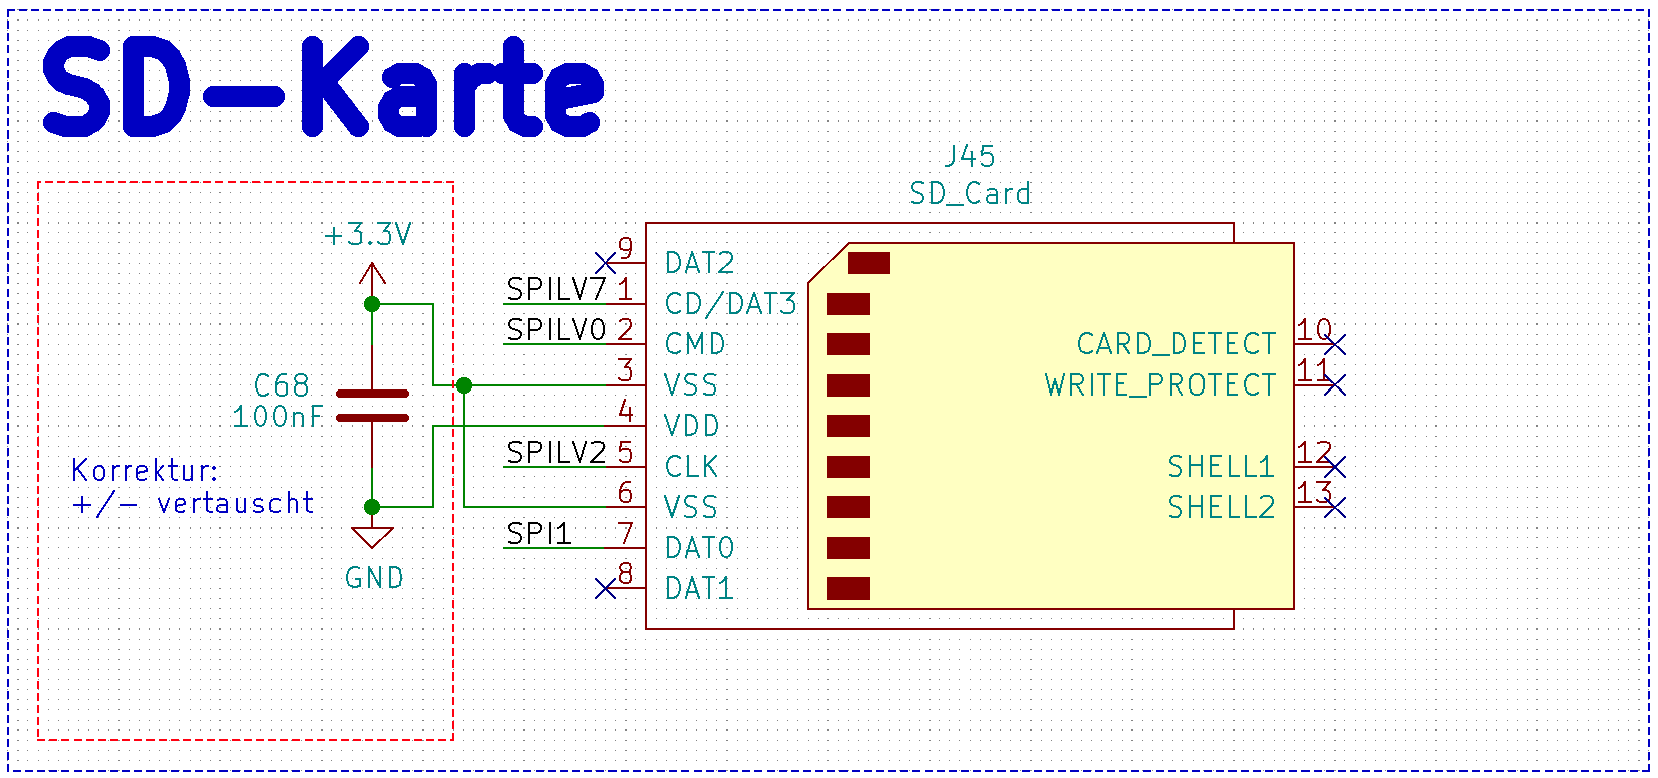
\includegraphics[width = 0.6 \textwidth]{graphics/Schema_SD_Karte}
\caption{Schema SD-Karte.}
\label{fig:Schema_SD_Karte}
\end{figure}

\paragraph{Funktionsbeschrieb der Schaltung}\mbox{}

In der Schaltung ist erkennbar, dass die SPI-Leitungen an die Pins des Adapters führen, genauso die Spannungsleitungen. Da die SD-Karte stets vom Mikrocontroller angesteuert wird, gibt es keine weiteren erwähnenswerte Funktionen zu beschreiben.

\section{Inbetriebnahme}
\label{sec:Inbetriebnahme}

Ein essentieller Teil der Entwicklung ist die Inbetriebnahme. Dabei wurden die Teilsysteme nacheinander in Betrieb genommen. Die einzelnen Systeme wurden dann in ihren wichtigsten Funktionen geprüft und für den Einsatz vorbereitet. In den folgenden Kapiteln wurden die einzelnen Teilsysteme der Cocktailmaschine in Betrieb genommen. 

\subsection{Speisungen}
\label{subsec:Inbetriebnahme_Speisungen}

Um die Speisungen in Betrieb nehmen zu können, ist gemäss Kapitel \ref{subsec:Speisungen} ein Jumper in die Schaltung implementiert worden, welcher die Speisungen von der übrigen Hardware trennt. Ausserdem sind Status-LED's verbaut, welche den korrekten Betrieb anzeigen sollen. Da es sich bei der 48V-Speisung um ein fertiges Netzteil handelt, musste dieses nicht grossartig in Betrieb genommen werden. Die einzige Einstellung, welche vorgenommen werden musste, ist die Feinjustierung der Ausgangsspannung mittels Drehregler am Netzteil.


\subsubsection{12V Speisung}
\label{subsubsec:Inbetriebnahme_12V_Speisungen}

Die 12V Speisung wurde für die Inbetriebnahme vom übrigen System abgekoppelt. Da diese aus der 48V-Speisung generiert wird, wurde lediglich diese vorgeschaltet. Beim Einschalten des Netzteils war der korrekte Betrieb am Status-LED sichtbar. Eine Messung mit dem Voltmeter bestätigte dies. Um allfällige Rippel sehen zu können, wurde noch mit dem Oszilloskop gemessen.



\subsubsection{5V Speisung}
\label{subsubsec:Inbetriebnahme_5V_Speisungen}

Simultan zur 12V-Speisung wurde die 5V-Speisung in Betrieb genommen. Auch bei dieser Speisung wurde lediglich das Netzteil vorgeschaltet und das restliche System abgeschnitten. Auch hierbei leuchtete das Status-LED sofort auf. Um zu verifizieren ob die richtige Spannung anliegt, wurde dies auch hier mit einem Voltmeter geprüft.

\subsubsection{3.3V Speisung}
\label{subsubsec:Inbetriebnahme_3.3V_Speisungen}



\newpage
\subsection{Programmierschnittstellen}
\label{sec:Inbetriebnahme_Programmierschnittstellen}

Die Programmierschnittstellen werden jeweils mithilfe einen USB-UART-Controller gesteuert. Im Folgenden wird die Inbetriebnahme dieser Schnittstelle für den Mikrocontroller ATMega2560 und das Bluetooth-/Wifimodul ESP32 beschrieben. Beide werden über eine USB-B-Buchse realisiert.

Für die Inbetriebnahme der USB-B-Schnittstelle wurde vorerst geprüft, ob der USB-UART-Converter über die USB-Buchse und Kabel vom Computer erkannt wird. Danach wurde geprüft, wie der Handshake beim Programmieren der Komponenten funktioniert. Die Inbetriebnahme der Programmierung wird in den Kapitel \ref{subsubsec:Inbetriebnahme_ESP} und Kapitel \ref{subsec:Inbetriebnahme_Mikrocontroller} beschrieben. Dies geschieht parallel, denn die Programme zum Schreiben, Kompilieren und Hochladen des Codes müssen schon vor dem Prüfen der USB-B-Schnittstelle installiert sein. Für die Inbetriebnahme wurde entschieden, dass der Handshake noch zum USB-B-Teil gehört und als Voraussetzung zählt, sodass das Programm überhaupt hochgeladen werden kann. Ausserdem wird dieser Handshake unabhängig davon gemacht, ob ein Device angehängt ist oder nicht. Erst nach einer Überprüfung der Device-Nummer kann bestimmt werden, ob das Target (ESP32 und ATMega2560) vorhanden ist oder nicht. Um den Handshake zu kontrollieren sind die in Abbildung \ref{fig:USB_B_Print} eingekreisten Punkte interessant:


\begin{figure}[h!]
\center
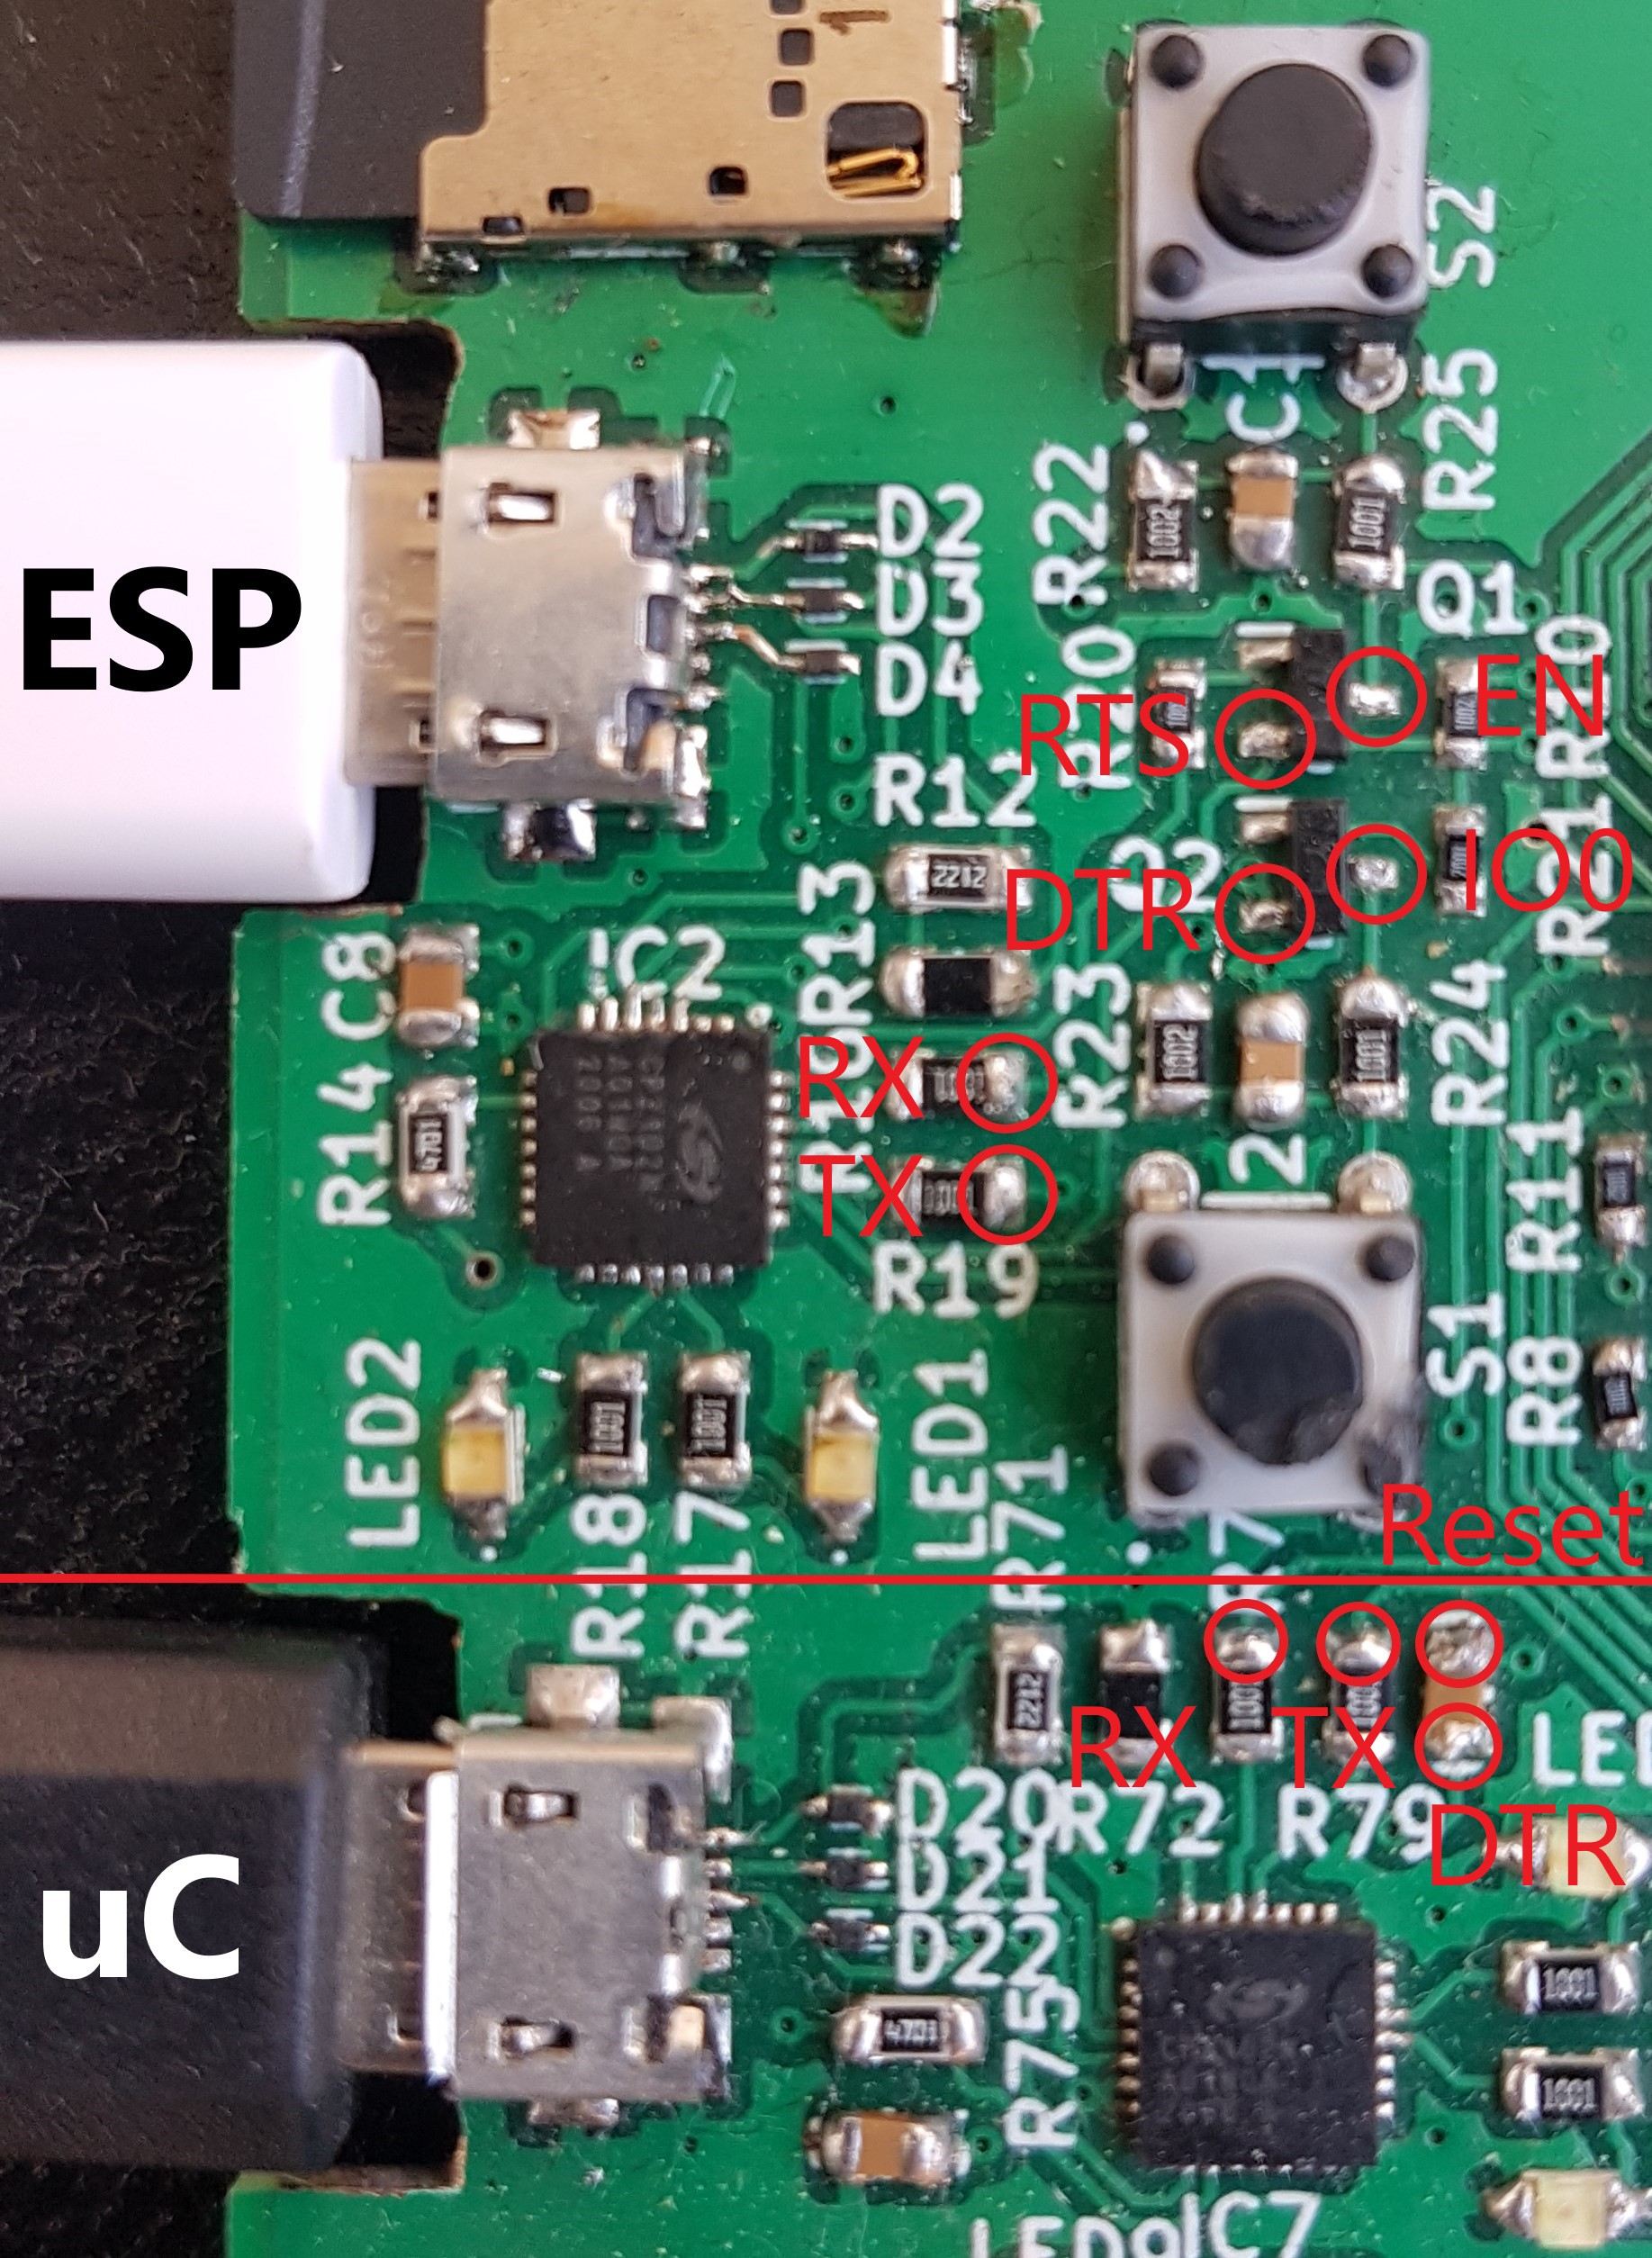
\includegraphics[width = 0.58\textwidth]{graphics/USB_B_Print}
\caption{Ausschnitt aus Platine (USB-Scnittstellen) mit eingekreisten Messpunkten.}
\label{fig:USB_B_Print}
\end{figure}

\todo{Kim bitte bessere Bildmarkierungen einfügen, welche besser sichtbar sind. Danke}

Für die Inbetriebnahme der Programmierschnittstellen wurde mit der entsprechenden Programmierumgebung ein HEX-File mit dem darin enthaltenen Code übertragen und die in Abbildung \ref{fig:USB_B_Print} markierten Punkte gemessen.

Folgende Schritte wurden befolgt:

\begin{enumerate}
\item Platine mit Spannung versorgen und Computer mit zwei USB-Kabeln an die USB-B-Buchsen anschliessen.\\
\textcolor{blue}{Systemeinstellungen\textrightarrow Geräte-Manager}\\
Dort sind die Devices sichtbar unter dem Name: \textit{Silicon Labs CP210x USB to UART Bridge}. Die Verifizierung ist im Anhang Kapitel \ref{Appendix:Geraete_Manager} zu finden.\newline
\item Überprüfen der Handshakes, welche definiert sind in den Tools zum Hochladen der Software.\\

\begin{enumerate}
\item ATMega2560\\

Um zu evaluieren, wie der Handshake durchgeführt wird, wurde beim Hochladen eines Programms an den markierten Punkten auf der unteren Seite in Abbildung \ref{fig:USB_B_Print} gemessen.\\

Im Anhang Kapitel \ref{Appendix:Handshake_uC} ist der Handshake und die Übertragung der ersten Bytes zu sehen. Der Handshake wird in einer weiteren Abbildung des selben Kapitels genauer aufgezeigt. Darin ist erkennbar, dass sobald die DTR-Leitung auf GND gezogen wird und die Spannung über dem Reset-Pin aufgrund des Kondensators zwischen DTR und Reset nur kurzzeitig auf 0V fällt. Dies reicht jedoch aus, dass der Mikrocontroller in den Boot-Modus fällt. Nach ca. 50ms beginnt die Datenübertragung vom Computer in den Flash-Speicher des uC.\\

\item ESP32\\

Um zu evaluieren, wie der Handshake durchgeführt wird, wurde beim Hochladen eines Programms an den markierten Punkten auf der oberen Seite in Abbildung \ref{fig:USB_B_Print} gemessen.\\

Im Anhang Kapitel \ref{Appendix:Handshake_ESP_Messung} wurden die ersten 100ms des Hochladen eines Programms auf das ESP32 gemessen. Gesucht wird nach einem gleichzeitigen Flankenwechsel der RTS-Leitung von 0 auf 1 und der DTR-Leitung von 1 nach 0. Eine weitere Abbildung im selben Kapitel zeigt eine genauere Aufnahme zum Zeitpunkt des Flankenwechsels.

Was bei genauerem Betrachten der Messungen auffällt: Entgegen der Erwartung ist der Flankenwechsel der beiden Leitungen leicht verzögert (um ca. 80 \textmu s). Auch das Signal des EN-Pins erreicht wesentlich schneller einen HIGH-Zustand als erwartet. Denn gemäss der Theorie müssen die Pins EN und IO0 zum gleichen Zeitpunkt auf LOW sein, um in den Download-Boot-Modus zu kommen, und trotz der Abweichung der Praxis zur Theorie funktioniert die Übertragung des Codes. Eine kleine Erläuterung zu dieser Abweichung ist im Anhang Kapitel \ref{Appendix:Handshake_ESP_Messung} zu finden. Schlussfolgerung davon ist, dass die Strapping-Pins wahrscheinlich erst nach einer gewissen Zeit gelesen werden und so die angelegten Zustände erst zu einem späteren Zeitpunkt von Bedeutung sind.

\end{enumerate}

\end{enumerate}


\subsubsection{USB-B}
\label{subsubsec:Inbetriebnahme_USB-B}

Für die Inbetriebnahme der USB-B-Schnittstelle wurde vorerst geprüft, ob der USB-UART-Converter über die USB-Buchse und Kabel vom Computer erkannt wird. Danach wurde geprüft, wie sich der Handshake beim Programmieren der Komponenten funktioniert. Das Inbetriebnahme der Programmierung wird in den Kapitel \ref{subsubsec:Inbetriebnahme_ESP} (WiFi-Modul) und Kapitel \ref{subsubsec:Inbetriebnahme_uC_Vorgehen} (Mikrocontroller) beschrieben. Dies geschieht ein wenig parallel, denn die Programme zum Schreiben, Kompilieren und Hochladen des Codes müssen schon vor dem Prüfen der USB-B-Schnittstelle installiert sein. Für die Inbetriebnahme wurde entschieden, dass der Handshake noch zum USB-B-Teil gehört und als Voraussetzung zählt, sodass das Programm überhaupt hochgeladen werden kann. Ausserdem wird dieser Handshake unabhängig davon gemacht, ob ein Device angehäng ist oder nicht. Erst nach einer Überprüfung der Device-Nummer kann bestimmt werden, ob das Target (ESP32 und ATMega2560) vorhanden ist oder nicht. Um den Handshake zu kontrollieren sind die in Abbildung \ref{fig:USB_B_Print} eingekreisten Punkte interessant:


\begin{figure}[h!]
\center
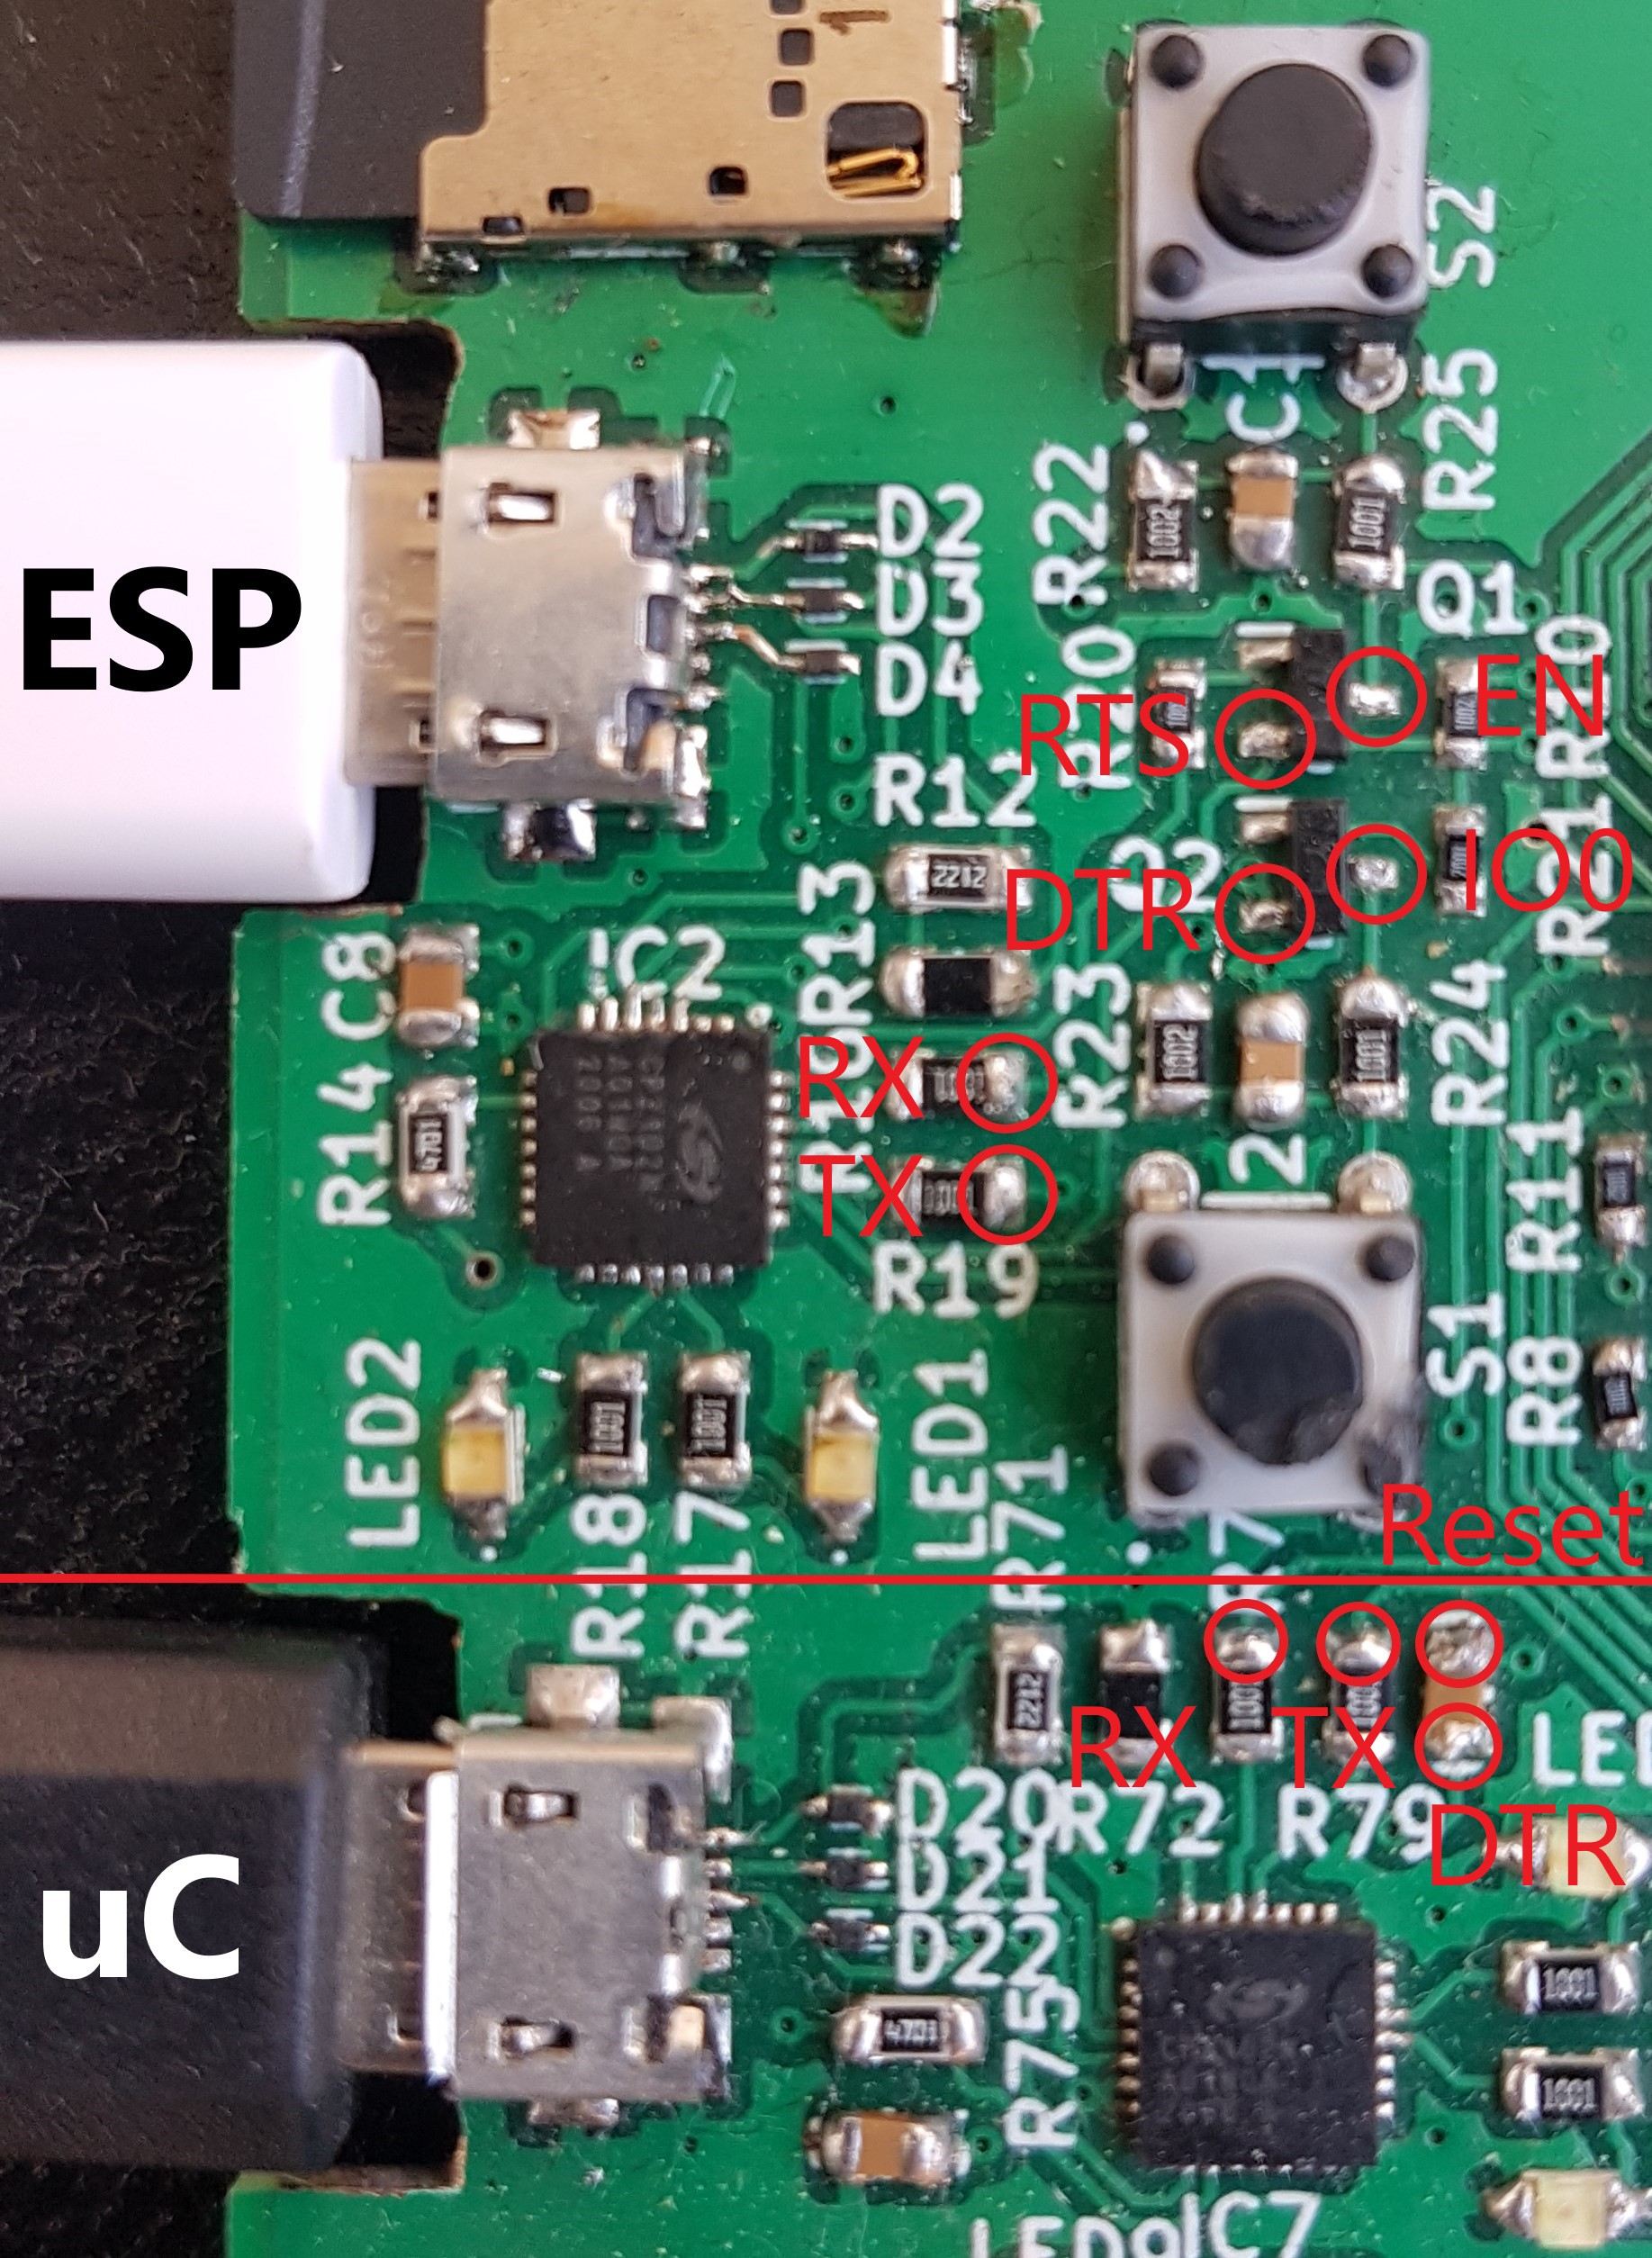
\includegraphics[width = 0.58\textwidth]{graphics/USB_B_Print}
\caption{Ausschnitt aus Platine (USB-Scnittstellen) mit eingekreisten Messpunkten.}
\label{fig:USB_B_Print}
\end{figure}
\newpage
Folgende Schritte wurden befolgt:

\begin{enumerate}
\item Platine mit Spannung versorgen und Computer mit zwei USB-Kabeln an die USB-B-Buchsen anschliessen.\\
\textcolor{blue}{Systemeinstellungen \textrightarrow Geräte-Manager} (siehe Abbildung \ref{fig:USB_Devices_Ger_Man})\\
Dort sind die Devices sichtbar unter dem Name: \textit{Silicon Labs CP210x USB to UART Bridge}\newline

\item Überprüfen der Handshakes, welche definiert sind in den Tools zum Hochladen der Software.

\begin{enumerate}
\item ATMega2560\\
Um herauszufinden, ob und wie der Handshake durchgeführt wird, wurde beim Hochladen eines Programms an den folgenden Leitungen gemessen:\\

\begin{tabular}{lcl}
1 & Gelb & DTR\\
2 & Blau & Reset\\
3 & Violett & RX\\
4 & Grün & TX\\
\\
\end{tabular}
In Abbildung \ref{fig:ATMega2560_DTR_RESET_RX_TX_gesamt} ist die Kommunikation mit den ersten Bytes zu sehen, in Abbildung \ref{fig:ATMega2560_DTR_RESET_RX_TX_1} wird der Handshake genauer aufgezeigt. Sobald die DTR-Leitung auf GND gezogen wird, fällt die Spannung über dem Reset-Pin aufgrund des Kondensators zwischen DTR und Reset nur kurzzeitig. Dies reicht jedoch aus, dass der Mikrocontroller in den Boot-Modus fällt. Nach ca. 50ms beginnt die Datenübertragung vom Computer in den Flash-Speicher des uC.

\begin{figure}[h!]
\center
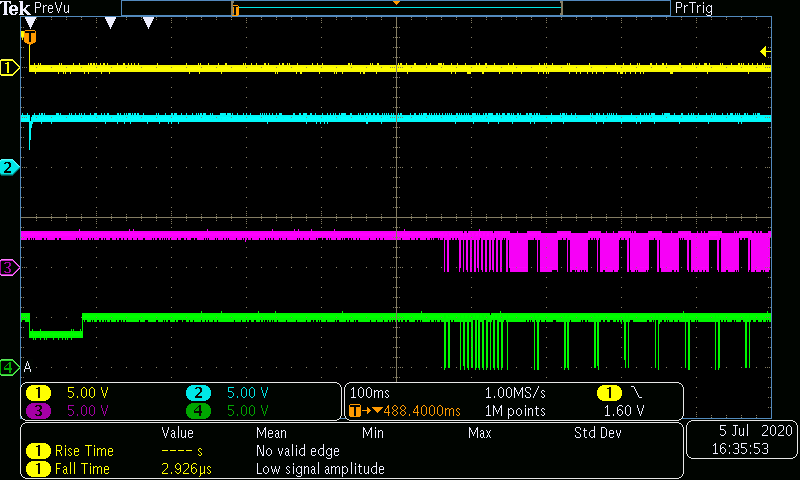
\includegraphics[width = \textwidth]{graphics/ATMega2560_DTR_RESET_RX_TX_gesamt}
\caption{Hochladen des Programmcodes auf den ATMega2560.}
\label{fig:ATMega2560_DTR_RESET_RX_TX_gesamt}
\end{figure}

\begin{figure}[h!]
\center
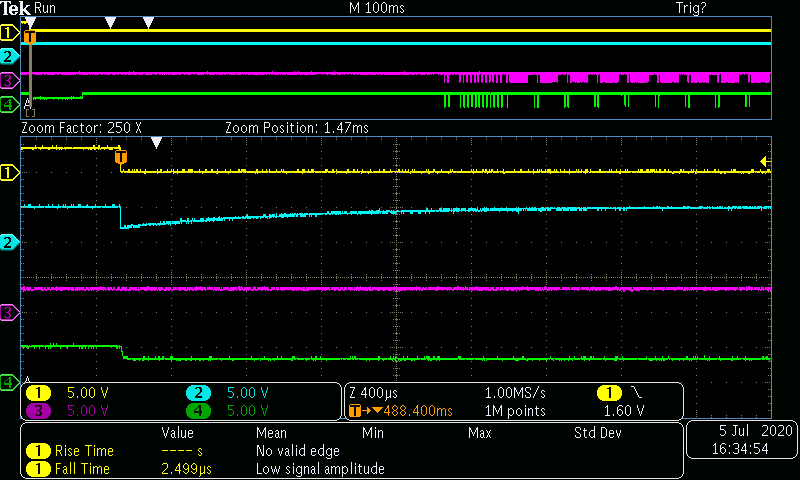
\includegraphics[width =  \textwidth]{graphics/ATMega2560_DTR_RESET_RX_TX_1}
\caption{Handshake zum Hochladen des Programmcodes auf den ATMega2560. Zoom auf den Moment des Resets.}
\label{fig:ATMega2560_DTR_RESET_RX_TX_1}
\end{figure}
\newpage
\item ESP32\\

Um herauszufinden, ob und wie der Handshake durchgeführt wird, wurde beim Hochladen eines Programms an den folgenden Leitungen gemessen:\\

\begin{tabular}{lcl}
1 & Gelb & RTS\\
2 & Blau & DTR\\
3 & Violett & EN\\
4 & Grün & IO0\\
\\
\end{tabular}

In Abbildung \ref{fig:ESP32_RTS_DTR_EN_IO0_gesamt} wurden die ersten 100ms des Hochladen eines Programms auf das ESP32 gemessen. Gesucht wird nach einem gleichzeitigen Flankenwechsel der RTS-Leitung von 0 auf 1 und der DTR-Leitung von 1 nach 0. Abbildung \ref{fig:ESP32_RTS_DTR_EN_IO0_2} zeigt eine genauere Aufnahme zum Zeitpunkt des Flankenwechsels.

Was auffält, ist dass entgegen der Erwartung der Flankenwechsel der beiden Leitungen leicht verzögert ist (um ca. 80 \textmu s). Auch das Signal des EN-Pins erreicht wesentlich schneller einen HIGH-Zustand als erwartet. Denn gemäss der Theorie müssen die Pins EN und IO0 zum gleichen Zeitpunkt auf LOW sein, um in den Download-Boot-Modus zu kommen, und trotz der Abweichung der Praxis zur Theorie funktioniert die Übertragung des Codes. Ein Fehler in der Matrix?

\newpage
\begin{table}[h!]
\center
\begin{tabular}{lcl|lcl|lcl|lcl}
1 & Gelb & RTS & 2 & Blau & DTR & 3 & Violett & EN & 4 & Grün & IO0\\
\end{tabular}
\end{table}
\begin{figure}[h!]
\center
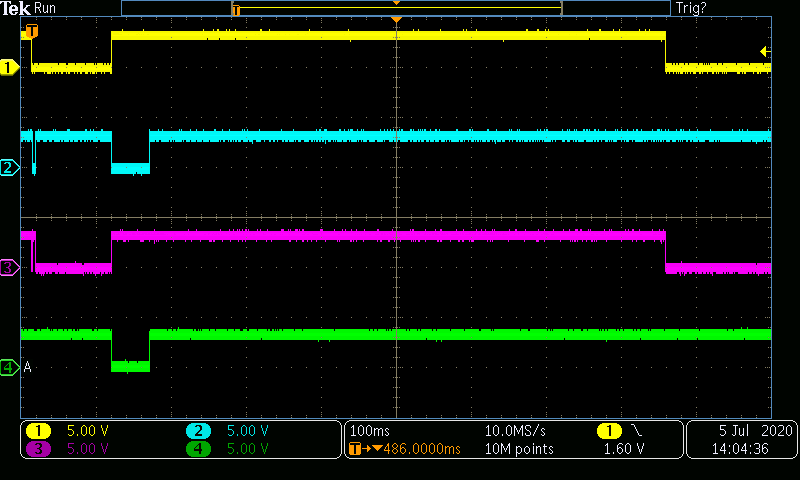
\includegraphics[width = \textwidth]{graphics/ESP32_RTS_DTR_EN_IO0_gesamt}
\caption{Handshake zum Hochladen des Programmcodes auf das ESP32.}
\label{fig:ESP32_RTS_DTR_EN_IO0_gesamt}
\end{figure}

\begin{figure}[h!]
\center
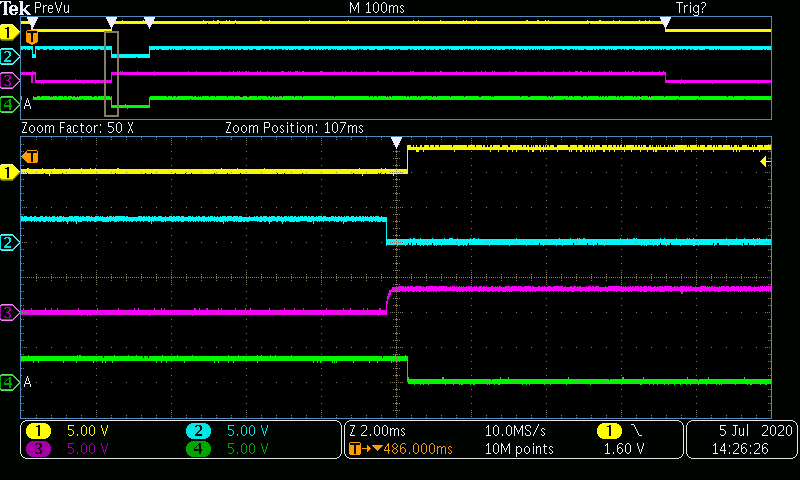
\includegraphics[width = \textwidth]{graphics/ESP32_RTS_DTR_EN_IO0_2}
\caption{Handshake zum Hochladen des Programmcodes auf das ESP32. Zoom auf gleichzeitiger Flankenwechsel RTS und DTR.}
\label{fig:ESP32_RTS_DTR_EN_IO0_2}
\end{figure}

\newpage

In einem Forum\footnote{https://forum.micropython.org/viewtopic.php?t=4607} wurde diese Auffälligkeit auch schon besprochen. Die Diskussion führte zum selben Ergebnis wie bei Inbetriebnahme. Nämlich, dass es nach dem Reset eine Zeit dauert, bis im Startprozess die Pins geprüft werden. Dazu gehört auch der Pin IO0. Somit ist es möglich, den Pin IO0 kurz nach dem Reset auf 0 zu ziehen.
Im selben Forum wurde auch die in Abbildung \ref{fig:ESP32_Handshake_Forum} gezeigte Darstellung gefunden. Ein Kommentar weist darauf hin, das mit dem esptool.py der EN-Pin des ESP32 direkt auf RTS gehängt werden kann. So lassen sich die Zeitpunkte, zu der die Pins auf 0 sind, näher zusammenschieben.

\begin{figure}[h!]
\center
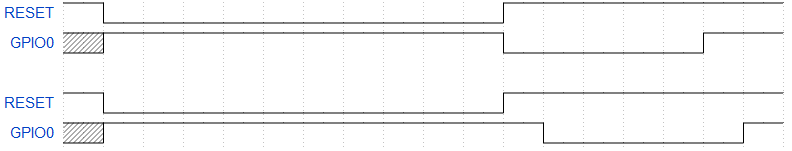
\includegraphics[width = \textwidth]{graphics/ESP32_Handshake_Forum}
\caption{Handshake zum Hochladen des Programmcodes auf das ESP32. Zoom auf gleichzeitiger Flankenwechsel RTS und DTR.}
\label{fig:ESP32_Handshake_Forum}
\end{figure}

Die Messung nach dem Einlöten der Brücke bestätigt dies, wie in Abbildung \ref{fig:ESP32_RTS_DTR_EN_IO0_mit_Bruecke_1} ersichtlich ist. Allerdings spielt der Kondensator jetzt nicht mehr so eine grosse Rolle, was auch nicht nötig ist. Auf das Hochladen des Codes hat die Brücke keinen Einfluss. Die Funktioniert wie bei der Schaltung ohne Brücke einwandfrei.
\begin{table}[h!]
\center
\begin{tabular}{lcl|lcl|lcl|lcl}
1 & Gelb & RTS & 2 & Blau & DTR & 3 & Violett & EN & 4 & Grün & IO0\\
\end{tabular}
\end{table}
\begin{figure}[h!]
\center
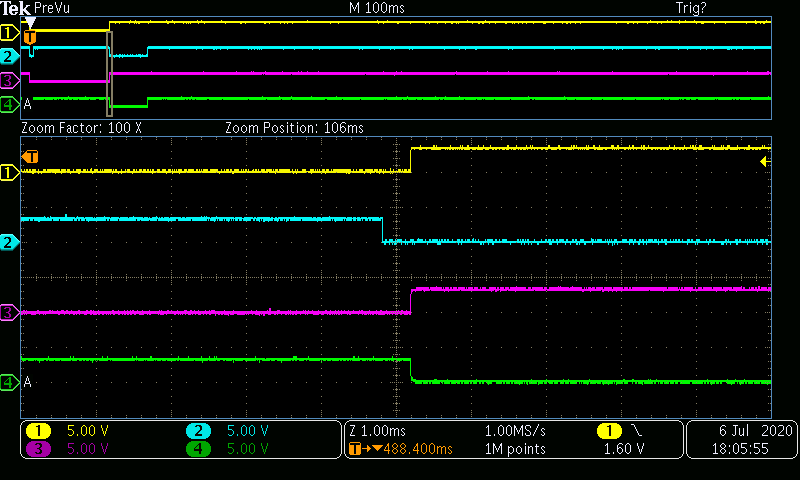
\includegraphics[width = \textwidth]{graphics/ESP32_RTS_DTR_EN_IO0_mit_Bruecke_1}
\caption{Handshake zum Hochladen des Programmcodes auf das ESP32. Zoom auf gleichzeitiger Flankenwechsel RTS und DTR.}
\label{fig:ESP32_RTS_DTR_EN_IO0_mit_Bruecke_1}
\end{figure}
\end{enumerate}

\end{enumerate}



\subsection{Benutzerschnittstellen}
\label{sec:Inbetriebnahme_Benutzerschnittstellen}

Im Folgenden wird die Inbetriebnahme der Benutzerschnittstellen erklärt. Dazu gehören das Display, das Wireless-/Bluetoothmodul und die RFID-Schnittstelle.

\subsubsection{Touch-Display}
\label{subsubsec:Inbetriebnahme_Touch_Display}

Der Test für das Display gestaltet sich am schnellsten. Die Schnittstelle wird mit dem schon im P5 geschriebenen Code getestet. Für den Test wird erwartet, dass ein Druck auf das Bild in der Mitte mit dem Cocktail eine Funktion auslöst. In dieser Funktion wird auf dem Display ein anderes Bild geladen und die Texte in den Buttons geändert. Eine andere Funktion simuliert eine Zubereitung eines Cocktails. Beide Funktionen haben gleich wie im P5 einwandfrei funktioniert.

\subsubsection{ESP}
\label{subsubsec:Inbetriebnahme_ESP}

Die Inbetriebnahme des ESP32-WROOM-32U geschieht mit der Programmierumgebung Arduino IDE. Um diesen in Betrieb nehmen zu können, waren einige Einstellungen und Downloads nötig, welche dann in der Arduino IDE eingebunden werden können. Es wird getestet, ob das ESP sich im vorgegebenen Netz anmeldet und als Webhost dient, ob bei Klicken auf ein Button im Explorer ein Event auslöst, ob die Kommunikation zwischen \textmu C und Mikrokontroller funktioniert.

Folgende Schritte wurden befolgt:
\begin{enumerate}
\item Benötigte Daten von Github\footnote{https://github.com/espressif/arduino-esp32} herunterladen.\newline
\item Dateien Entpacken und speichern unter:\newline
\textcolor{magenta}{C:\textbackslash Users \textbackslash ''Benutzer''\textbackslash Documents\textbackslash Arduino\textbackslash hardware \textbackslash espressif \textbackslash esp32}\newline
Damit die Arduino IDE die Files findet.\newline
\item Arduino IDE starten und folgenden Reiter öffnen:\newline
\textcolor{blue}{Arduino IDE \textrightarrow Werkzeuge \textrightarrow Board}\newline
ESP32 Dev Module auswählen.\newline
\item Unter demselben Reiter können noch weitere Einstellungen getätigt werden.\newline
\textcolor{blue}{Arduino IDE \textrightarrow Werkzeuge \textrightarrow ...}\newline
\begin{tabular}{lll}
Upload Speed & : & 921600\\
CPU Frequency & : & 240MHz\\
Flash Frequency & & 80MHz\\
Flash Mode & : & QIO\\
Flash Size & : & 4MB (32Mb)\\
Partition Scheme & : & Default 4MB wit spifss\\
Core Debug Level & : & none\\
PSRAM & : & disabled\\
Port & : & \textcolor{red}{COMx}\\
\end{tabular}

Wobei der Port \textcolor{red}{COMx} im Geräte-Manager ermittelt werden muss. Das ESP32 ist jetzt flashbar.\newline

\item Testprogramm herunterladen\footnote{https://randomnerdtutorials.com/esp32-web-server-arduino-ide/}, leicht modifizieren und hochladen.\newline
\textcolor{blue}{Arduino IDE \textrightarrow Verify and Upload Button} \newline
Für die Inbetriebnahme wurde das Testprogramm so modifiziert, dass das ESP32 gleich getestet werden kann wie das Touch-Display. Dies bedeutet, dass das ESP eine Page-ID, eine Button-ID und das Abschlusszeichen 0xFF 0xFF 0xFF sendet. Der Unteschied ist, dass das ESP über einen anderen UART-Port des \textmu C kommuniziert. Die Testsoftware ist bei den anderen Firmwares auf dem USB-Stick zu finden.\newline
\item Die ''Debug Kommunikation'' über den ersten Seriellen Port des ESP32 testen.

\textcolor{blue}{Arduino IDE \textrightarrow Tools \textrightarrow Serial Monitor}\newline
Im Testprogramm wird hier angezeigt, wenn ein neuer Client die IP-Adresse aufruft und wenn im Internetexplorer ein Button gedrückt wird. Erste Versuche nach dem hochladen waren erfolgreich, das ESP hat eine IP-Adresse zugeordnet bekommen.
\end{enumerate}

Über die zweite serielle Schnittstelle findet die Kommunikation zwischen ESP32 und Atmega2560 statt. Sobald über den Webserver eine Aktion ausgelöst wird, sendet das ESP die gleiche Zeichenfolge, welche auch das Display ausgibt. Der Test zeigt, dass das Drücken auf den Button im Internetexplorer die gleiche Aktion auslöst, wie das Drücken auf das Touch-Display. Es werden Bilder neu gesetzt und Texte geändert. Die Implementierung des EPS ist folglich erfolgreich.

\subsubsection{RFID}
\label{subsubsec:Inbetriebnahme_RFID}


\newpage
\subsection{Mikrocontroller}
\label{subsec:Inbetriebnahme_Mikrocontroller}

Um das Anwenderprogramm auf dem Mikrocontroller (\textmu C) speichern zu können, ist es am angenehmsten, wenn dies direkt aus der Programmierumgebung geschehen kann. Als Programmierumgebung wird aufgrund des AVR-Chips die Software Atmel Studio 7.0 ausgewählt.

\subsubsection{Bootloader}

Ein Bootloader (BL) ermöglicht seitens \textmu C den Programmiervorgang über USB und stellt sicher, dass der frisch kompilierte Code in den Programmspeicher des \textmu C gelangt. Im Grunde ist der BL ein Code am Beginn des Programmablaufs, welcher entsprechend nach einem Reset aufgerufen wird. Innerhalb des BL-Codes wird für zwei Sekunden auf eingehende Daten der UART0-Schnittstelle gewartet.
%Wenn innerhalb von ca. zwei Sekunden keine Daten ankommen, wird das Anwenderprogramm gestartet. 
Wird innerhalb dieser zwei Sekunden ein Anwenderprogramm in Form eines HEX-Files an den Mikrocontroller gesendet, wird es gemäss stk500v2-Protokoll \todo{cite: http://ww1.microchip.com/downloads/en/Appnotes/doc2591.pdf} in den Flash-Speicher geladen.
%Nach dem Laden in den Flash-Speicher wird das neu geladene Programm gestartet. 
Aufgrund des BL geht es nach einem Reset des \textmu Cs zwei Sekunden, bis das eigentliche Programm startet.

Für den \textmu C des Cocktailmixers wird ein stk500v2-BL verwendet. Dieser kann über Github\footnote{https://github.com/arduino/Arduino-stk500v2-bootloader/blob/master/stk500boot.c
} heruntergeladen werden. Im File stk500v2.c befinden sich einige Anweisungen, welche Fuse- und Lock-Bits wann gesetzt werden müssen. Achtung, die Angaben haben im Falle des Cocktailmixers nur mit Abweichungen funktioniert (4096 words anstelle 1024). Durch Anpassen des start-Vektors auf den Programmspeicher und Setzen der korrekten Bootloader-Fuses wäre es möglich, den BL-Speicherplatz zu verkleinern um den Programmspeicher zu vergrössern.

%Wie der Flash-Speicher grob organisiert ist wird in Abbildung \ref{fig:Flash_Speicher_uC} gezeicht. Der Flash-Speicher für den Bootloader, wird in eine No-Read-While-Write Section geschrieben. Das Anwendungsprogramm in die Read-While-Write Section.

%\begin{figure}[h!]
%	\centering
%	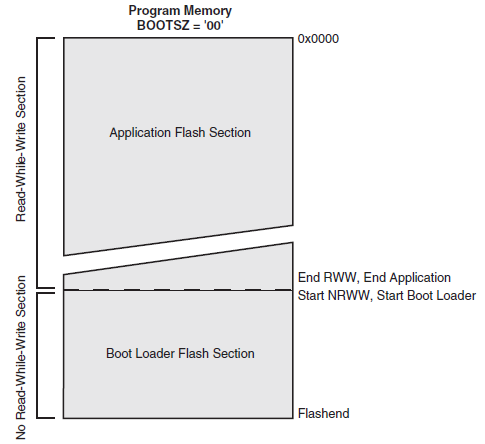
\includegraphics[width=0.8\textwidth]{graphics/Flash_Speicher_uC}
%	\caption{Flas-Speicher Mikrocontroller.}
%	\label{fig:Flash_Speicher_uC}
%\end{figure}
%\todo{cite: https://www.mikrocontroller.net/articles/AVR\_Bootloader\_in\_C\_-\_eine\_einfache\_Anleitung}
\subsubsection{Fuse-Bits}

%\begin{table}[h!]
%\center
%\begin{tabular}{|l|l|l|l|l|}
%\hline
%Bit & Register-Name & Default & Programmed & Mixer (0xFF)\\ \hline
%0 & BODLEVEL0 & 1 & 0 (1.8V) & 1\\
%1 & BODLEVEL1 & 1 & 0 (2.7V) & 1\\
%2 & BODLEVEL2 & 1 & 0 (4.3V) & 1\\
%3 & - & 1 & - & 1 \\
%4 & - & 1 & - & 1 \\
%5 & - & 1 & - & 1 \\
%6 & - & 1 & - & 1 \\
%7 & - & 1 & - & 1 \\ \hline
%\end{tabular}
%\label{tab:Extended_Fuses}
%\caption{Bits Etended Fuses.}
%\end{table}

%\begin{tabularx}{\textwidth}{ll|X}
%
%BODLEVEL0:2 				& : 	& Setzt die Brown-Out-Spannung. Sobald die Versorgungsspannung unterdiese Schwelle fällt, schaltet der uC aus. Für: 
%\begin{tabular}{lll}
%1.8V 		& = & 0b11111110\\
%2.7V 		& = & 0b11111101\\
%4.5V 		& = & 0b11111011\\
%disabled 	& = & 0b11111111
%\end{tabular}
%
%%\todo{cite: Atmel Datenblatt Seite 48}\\
%
%\end{tabularx}
%\todo{cite: Siehe Cites auskommentiert in Tabelle}

%\begin{table}[h!]
%\center
%\begin{tabular}{|l|l|l|l|l|l|l|l|l|}
%\hline
%Bit & Register-Name 	& Default 	& Programmed 							& Mixer (0xD0)\\ \hline
%0 	& BOOTRST  		& 1 			& 0 (Startet Bootloader bei Reset) 		& 0\\
%1 	& BOOTSZ0  		& 0 			& X (Definiert Bootloader-Speicherplatz) 	& 0\\
%2 	& BOOTSZ1  		& 0 			& X (Definiert Bootloader-Speicherplatz) 	& 0\\
%3 	& EESAVE  		& 1 			& 0 (Schützt EEPROM während Löschen) 	& 0\\
%4 	& WDTON 			& 1 			& 0 (Watchdog immer Ein)					& 1\\
%5 	& SPIEN 			& 0 			& 0 (Aktiviert ISP-Schnittstelle)		& 0\\
%6 	& JTAGEN 		& 0 			& 0 (Aktiviert JTAG-Schnittstelle) 		& 1\\
%7 	& OCDEN 			& 1 			& 0 (z.T Clock in Sleep-Modus) 			& 1\\ \hline
%\end{tabular}
%\label{tab:High_Byte_Fuses}
%\caption{Bits High-Byte-Fuses.}
%\end{table}

Da während dem Entwickeln die Möglichkeit bestehen soll, den Flash-Speicher per USB zu beschreiben, muss beim Aufstarten der BL aufgerufen werden. Dazu muss das BOOTRST-Bit aktiviert werden. Der Speicherplatz für den BL wird auf 4096 words gesetzt (anders als stk500v2 Erklärung). Das EEPROM soll beim Löschen des \textmu C geschützt bleiben, weshalb das EESAVE-Bit aktiviert wird. Da die ISP-Schnittstelle benötigt wird, um den BL zu schreiben und Fuse-Bits zu setzen, wird das SPIEN-Bit gesetzt.
%
%\begin{tabularx}{\textwidth}{ll|X}
%
%BOOTRST 	& : 	& 
%Nach Reset wird Programm von Bootloader-Memory-Section gestartet. Wenn ein Bootloader verwendet wird, um den Mikrocontroller zu flashen, muss dieses Bit aktiviert sein. \\ \hline
%
%%\todo{cite: https://embedds.com/all-you-need-to-know-about-avr-fuses/}\\
%
%BOOTSZ0:1 		& : &
%Definiert Bootloader-Grösse (je kleiner desto mehr Platz für Applikation). Grössen : 512, 1024,2048,4096 words.\\ \hline
%
%%\todo{cite: Atmel Datenblatt Seite 320}\\
%
%EESAVE 				& : & 
%Schütz EEPROM-Speicher währenddem der Chip gelöscht wird.\\ \hline
%
%%\todo{cite: https://embedds.com/all-you-need-to-know-about-avr-fuses/}\\
%
%
%WDON 				& : & 
%Forciert Chip-Reset, wenn nichts spezielles passiert.\\ \hline
%
%%\todo{cite: https://embedds.com/all-you-need-to-know-about-avr-fuses/}\\
%
%SPIEN 				& : & 
%Aktiviert die ISP-Schnittstelle. Don't touch!\\ \hline
%
%%\todo{cite: https://www.mikrocontroller.net/articles/AVR\_Fuses}\\
%
%JTAGEN 				& : & 
%Aktiviert die JTAG-Schnittstellt. Wird empfohlen auszuschalten wenn nicht benötigt.\\ \hline
%
%%\todo{cite: https://www.mikrocontroller.net/articles/AVR\_Fuses}\\
%
%OCDEN 				& : & 
%Ermöglicht gewissen Teilen des Clock-Systems während eines sleep-modus weiterhin zu laufen.\\
%
%%\todo{cite: Atmega2560 Datenblatt, Seite 327}\\
%
%\end{tabularx}
%\todo{cite: Siehe Cites auskommentiert in Tabelle}
%
%\begin{table}[h!]
%\center
%\begin{tabular}{|l|l|l|l|l|l|l|l|l|}
%\hline
%Bit & Register-Name 	& Default 	& Programmed 						& Mixer (0xF7)\\ \hline
%0 	& CKDIV8 		& 0 			& 0 (System-Clock-Prescaler = 8)		& 0\\
%1 	& CKOUT  		& 1 			& 0 (PE7 als System-Clock-Output) 	& 1\\
%2 	& SUT1			& 1 			& X (Aufstartzeit) 					& 0\\
%3 	& SUT0			& 0 			& X (Aufstartzeit) 					& 0\\
%4 	& CKSEL3			& 0 			& X (Frequenzbereich)				& 1\\
%5 	& CKSEL2			& 0 			& X (Frequenzbereich)				& 1\\
%6 	& CKSEL1			& 1 			& X (Frequenzbereich)				& 1\\
%7 	& CKSEL0			& 0 			& X (Aufstartzeit)					& 0\\
%\hline
%\end{tabular}
%\label{tab:Low_Byte_Fuses}
%\caption{Bits Low-Byte-Fuses.}
%\end{table}
%
Für den \textmu C verwenden wir einen 16MHz Full-Swing-Crystal-Oszillator, weshalb die Bits CKSEL3:1 auf 111 stehen müssen.
Die Aufstartzeit wird vorsorglich auf die längst mögliche Zeit eingestellt. Dies führt dazu, dass das Register CKSEL0 auf 0 und die Register SUT0:1 auf 00 gesetzt werden.
%
%
%\begin{tabularx}{\textwidth}{ll|X}
%
%CKDIV8 				& : 	& Setzt den Initialwert des System-Clock-Prescalers auf 8.
%\\ \hline
%
%%\todo{cite: Atmel Datenblatt Seite 48}\\
%
%CKOUT 				& : & Setzt den Pin PE7 als System-Clock-Output.
%\\ \hline
%
%%\todo{cite: Atmega Datenblatt Seite 327}\\
%
%SUT0:1 				& : & Setzt Parameter zur Aufstartzeit.
%\\ \hline
%
%%\todo{cite: Atmel Datenblatt Seite 42}\\
%
%CKSEL0:3 			& : & Setzt Parameter zum Oszillator (CKSEL1:3) und Aufstartzeit (CKSEL0).
%\\ \hline
%
%%\todo{cite: Atmel Datenblatt Seite 42}\\
%
%\end{tabularx}
%\todo{cite: Siehe Cites auskommentiert in Tabelle}
%
Der Brown-out-Detektor setzt den internen Reset, sobald die Versorgungsspannung unter einen Wert fällt. Wenn der Mikrocontroller ausfällt, während der TMC4671 noch aktiv ist, wird der Motor weiter gefahren. Dieses Risiko soll eingeschränkt werden, indem dieser Modus ausgeschaltet wird.

Die Lock-Bits müssen gesetzt werden, nachdem der BL in den Speicher geschrieben wurde. ''SPM ist nicht erlaubt, in den Anwenderbereich zu schreiben und LPM ist nicht erlaubt aus dem Applikationssktor zu lesen, wenn LPM aus dem Urlader-Bereich ausgeführt wird.''

\todo{cite : https://www-user.tu-chemnitz.de/~heha/viewchm.php/hs/ATmegaX8.chm/28.htm}
\newpage
Daraus folgt für die Fuse- und Lock-Bits die Einstellungen gemäss Tabelle \ref{tab:Fuse_und_Lock-Bits}. Siehe Anhang \ref{Appendix:Mikrocontroller} und \ref{Appendix:Atmel_Studio} für Details.

\begin{table}[h!]
\center
\begin{tabular}{|l|l|l|l|}
\hline
\textbf{Extended} & \textbf{High} & \textbf{Low} & \textbf{Lock}\\
\hline
0xFF & 0xD0 & 0xF7 & 0xCF\\
\hline
\end{tabular}
\caption{Tabelle Fuse- und Lock-Bits.}
\label{tab:Fuse_und_Lock-Bits}
\end{table}


\subsubsection{AVRdude in Atmel Studio einbinden}\label{subsubsec:avrdude_in_atmelstudio_einbinden}

AVRdude ist eine Software, mit der Atmel AVR Controller programmiert werden können. Sie schreibt den bereits kompilierten HEX-Code der Programmierumgebung über den Bootloader in den Flash-Speicher des Controllers. Hier gäbe es auch eine Methode, die Fuse- und Lock-Bits des \textmu C zu setzen.

\todo{https://www.mikrocontroller.net/articles/AVRDUDE}

Über einen Link\footnote{http://download.savannah.gnu.org/releases/avrdude/} kann eine Datei heruntergeladen werden in Form von \textcolor{blue}{avrdude-6.3-mingw32.zip}. Der gleichnahmige Ordner wird im Ordner \textcolor{blue}{C:\textbackslash Tools} gespeichert. Danach wird in AtmelStudio der Reiter ''\textcolor{blue}{Tools\textrightarrow External Tools}'' ausgewählt und ein neues Tool hinzugefügt. Im Falle des Atmega2560 geben wir die Commands gemäss Tabelle \ref{tab:AVRdude_commands} ein:

\begin{table}[h!]
\center
\begin{tabularx}{\textwidth}{|l|l|X|}
\hline
Title & : & Cocktailmixer \\
\hline
Command & : & C:\textbackslash Tools\textbackslash avrdude-6.1-mingw32\textbackslash avrdude.exe \\
\hline
Arguments: & : & -D -P \textcolor{red}{ COMx} -p ATMEGA2560 -c wiring -b 115200 -U flash:w:\$(TargetDir)\$(TargetName).hex:i\\
\hline
\end{tabularx}
\caption{AVRdude Commands}
\label{tab:AVRdude_commands}
\end{table}

Der entsprechende \textcolor{red}{ COMx}-Port des zu flashenden Gerätes (Atmega2560) muss mit dem Geräte-Manager ermittelt werden.

\todo{cite Herr Meier Skript mc1}


Sämtliche Tabellen aus dem Datenblatt und Screenshots aus Programmierumgebung, welche mit dem Setzen der Fuse- und Lock-Bits oder Programmierung des \textmu C zusammenhängen, sind im Anhang Kapitel \ref{Appendix:Mikrocontroller} angefügt.

\subsubsection{Vorgehen}\label{subsubsec:Inbetriebnahme_uC_Vorgehen}

\begin{enumerate}
\item Als Erstes wurden die Fuse-Bits gesetzt. Dies geschah über den Reiter:\newline
\textcolor{blue}{AtmelStudio \textrightarrow Tools \textrightarrow Device programming \textrightarrow Fuses} (siehe Abbildung \ref{fig:AtmelStudio_Fuses}) \newline
Es wurde darauf geachtet, dass der AVR mkII ausgewählt wurde und der Gerätecode des Atmega2560 ausgelesen werden konnte.
\newline
\item Als Zweites wurde der Bootloader installiert. Dies geschah unter:\newline
\textcolor{blue}{AtmelStudio \textrightarrow Tools \textrightarrow Device programming \textrightarrow Memory} (siehe Abbildung \ref{fig:AtmelStudio_Program_Bootloader}) \newline
Hier wird ein stk500v2-BL verwendet, kann aber auch abweichen. (Entsprechende Anpassungen nötig, nicht Teil dieses Projektes.)\newline
\item Als Drittes wurden die Lock-Bits gesetzt unter:\newline
\textcolor{blue}{AtmelStudio \textrightarrow Tools \textrightarrow Device programming \textrightarrow Lock-Bits} (siehe Abbildung \ref{fig:AtmelStudio_Locks})\newline
Diese sollten nicht mehr geändert werden. Bei jedem Brennen des BL wieder zu setzen.\newline
\item Ggf. USB-Firmware installieren auf dem USB-UART-Converter. (Nicht Teil dieses Projektes.)\newline
\item Mikrocontroller mit der kompillierten Software (Cocktailmixer.HEX) programmieren.\newline
\textcolor{blue}{AtmelStudio \textrightarrow Tools \textrightarrow Cocktailmixer})\newline
Alternativ direkt mit ISP-Programmer wie in Schritt 2 (ohne Bootloader, Programmcode an start-Vektor des \textmu Cs.):\newline
\textcolor{magenta}{z.B C:\textbackslash Users\textbackslash DaU\textbackslash Software\textbackslash Cocktailmixer\textbackslash Cocktailmixer\textbackslash Debug\textbackslash Cocktailmixer.HEX}
\end{enumerate}

Das Setzen der Fuse- und Lock-Bits sowie das brennen des Bootloaders kann mit einem AVR MKII Programmer in Atmel Studio gemacht werden. Alternativ gibt es einen Weg, den USB-Treiber (Atmega16U2) eines Arduino Uno mit einer entsprechenden Firmware zu laden, sodass dieser als Programmer verwendet werden kann\footnote{https://www.instructables.com/id/Turn-Arduinos-Serial-Converter-Into-AVRISP-MkII-Cl/}.

Für die Inbetriebnahme des Mikrocontrollers wurde der Alternativweg gewählt. Die Ergebnisse können sich zeigen lassen. Der Mikrocontroller ist programmierbar und erste Tests mit der Software waren erfolgreich, das Programm wurde auch ordnungsgemäss gestartet. Dies wurde geprüft, indem der während dem Projekt 5 erarbeitete Code hochgeladen wurde.

Wird der Mikrocontroller per Reset-Button neu gestartet, dauert es aufgrund des Bootloaders 2s, bis der Programmcode gestartet wird. Während dieser Zeit wartet der Bootloader auf einkommende Daten, welche auf den Flash-Speicher geschrieben werden sollen. Danach startet das Programm, sollten keine Daten kommen.

\subsubsection{Messungen}

Die Messung des Oszillator-Eingangs ergab eine saubere harmonische Schwingung mit 16MHz, abgebildet in Abbildung \ref{fig:Crystal_Swing}. 

\begin{figure}[h!]
\center
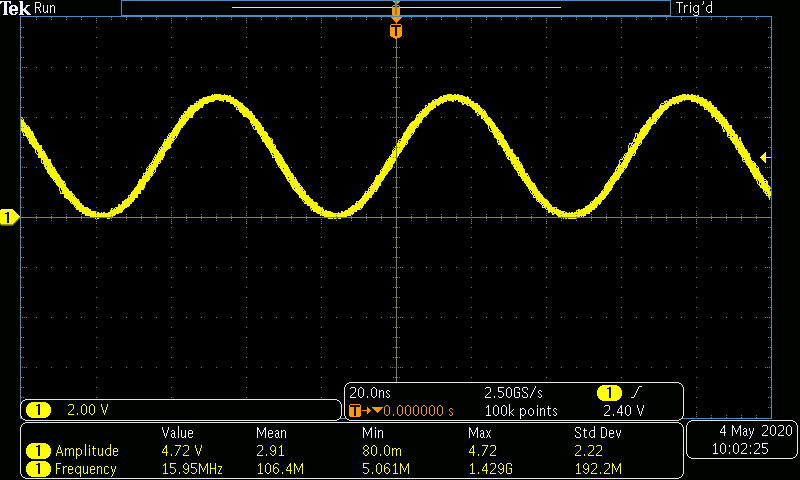
\includegraphics[width = 0.8\textwidth]{graphics/Crystal_Swing}
\caption{Schwingung des Oszillators}
\label{fig:Crystal_Swing}
\end{figure}

\newpage
\subsection{Datenspeicherung}
\label{sec:Inbetriebnahme_Datenspeicherung}

Im Folgenden wird die Datenspeicherung in Betrieb genommen. Dies geschieht mit dem Programm, welches in der Library vorhanden ist. Damit kann auf das Directory Table zugegriffen werden und die darauf vorhandenen Files gelesen und bearbeitet werden. Es können auch neue Files generiert werden.

Die benutzte Library ist eine ältere Version. Die neueren Versionen sind auf der Homepage gezeigt und bieten einen noch breiteren Verwendungszweck. Ein wirklich gelungenes Projekt. \cite{dharmani_sdsdhc_2009}

\subsubsection{mikroSD-Karte}
\label{subsubsec:Inbetriebnahme_mikroSD_Karte}

Die Inbetriebnahme der mikroSD-Karte geschieht mit einem Testprogramm. Das Programm initialisiert die benötigte Hardware (SPI, UART, Pins), enthält eine FAT32-Library und ermöglicht das Debugen über die serielle Schnittstelle.

Sobald die interne Hardware der Mikrocontrollers initialisiert ist, wird die SD-Karte gebootet. Hat dies funktioniert, wird ein File namens \textit{TEST.txt} erstellt, welches den String \textit{Hallo File} enthält.

Vorgehen:
\begin{enumerate}
\item Benötigte Applikation, welche im Software-Ordner auf dem USB-Stick oder Github \cite{aebi_projekt-6softwareatmega_2020} zu finden ist, in Atmel Studio öffnen.\\
\textcolor{magenta}{Software\textrightarrow Atmega\textrightarrow  2\_SD\_Karte \textrightarrow SD\_Karte}\\

\item Software hochladen:\\
\textcolor{blue}{AtmelStudio \textrightarrow Tools \textrightarrow PartyMixer}\\

\item Programm für Kommunikation über die serielle Schnittstelle downloaden (z.B HTerm 0.8.1beta.)\cite{hammer_hterm_nodate}\\
\item Verbindung mit Mikrocontroller herstellen und Neustart über Button DTR auslösen. Damit wird der DTR-Pin getoggelt und der Mikrocontroller neu gestartet\\

\begin{table}[h!]
\center
\begin{tabular}{lcl}
Port & = & \textcolor{red}{COMx} \\
Baudrate & = & 57600 \\
Data & = & 8 \\
Stop & = & 1 \\
\end{tabular}
\end{table}

Der Port \textcolor{red}{COMx} ist aus dem Geräte-Manager zu entnehmen. Es ist derselbe Port, welcher verwendet wird um die Software hochzuladen.\\

\end{enumerate}

Ergebnis: Die mikroSD-Karte wird erfolgreich gebootet, was im seriellen Monitor mit ''Boot...OK!'' angezeigt wird. Das File namens \textit{TEST.txt} mit dem Textinhalt \textit{Hallo File} ist jetzt auf der SD-Karte vorhanden.

\subsection{Flüssigkeitsbeförderung}
\label{subsec:Inbetriebnahme_Flüssigkeitsbeförderung}



\subsubsection{Pumpen}
\label{subsubsec:Inbetriebnahme_Pumpen}

Um die Flüssigkeitsbeförderung zu testen, wurde ein Testprogramm erstellt, welches die 12 Pumpen der Reihe nach für eine kurze Zeitdauer einschaltet. Dies funktionierte auf Anhieb und es konnten einige Tests durchgeführt werden. 

Einer der wichtigsten Tests war es dabei, den maximalen Durchfluss der Pumpen zu bestimmen. Dies ermöglichte eine Abschätzung, wie lange es benötigt um einen Cocktail herzustellen. Um das Pflichtziel von unter einer Minute erfüllen zu können, müssen daher die Pumpen genügend schnell Pumpen können.

Im Schnitt ergab sich dabei eine Abfüllzeit von 26 Sekunden für eine Menge von 5dl. Erstaunlich ist jedoch, dass die Pumpen unterschiedlich lange benötigen für die selbe Menge. Somit benötigte die langsamste Pumpe 28 Sekunden, wobei die schnellste Pumpe lediglich 24 Sekunden benötigte. Das Zusammenspiel von Pumpen und Motor wird in der Zielerreichung in Kapitel \ref{sec:Zielerreichung} aufgezeigt.

\subsubsection{Durchflussmessgeräte}
\label{subsubsec:Inbetriebnahme_Durchflussmessgeräte}

Die Durchflussmessgeräte in Betrieb zu nehmen gestaltete sich ein wenig schwieriger als bei den Pumpen in Kapitel \ref{subsubsec:Inbetriebnahme_Pumpen}. Da die Durchflussmessgeräte bei Durchfluss Pulse ausgeben, müssen die positiven Flanken gezählt werden. Dafür wurde das Testprogramm für die Pumpen erweitert. Auch dies funktionierte auf Anhieb und es konnte mit ersten Testläufen begonnen werden. 

Da die Durchflussmessgeräte auf dem volumetrischen Prinzip basieren, spielt es keine Rolle ob die 12 Pumpe exakt gleich stark Pumpen oder nicht. Es wurde jedoch schnell festgestellt, dass die Durchflussmessgeräte kleine Toleranzen zueinander aufweisen, jedoch für sich selber relativ exakt arbeiten. Dies hatte zur folge, dass die einzelnen Durchflussmessgeräte jeweils separat mit der Software kalibriert werden mussten. Dabei ist aufgefallen, dass die Anzahl der Pulse im Verhältnis zum Volumen für die einzelnen Durchflussmessgeräte auch nicht ganz linear ist. Somit wurden zwei Kalibrierungen pro Durchflussmessgerät vorgenommen. Einmal wurden die Durchflussmessgeräte auf 3dl und einmal auf 5dl kalibriert. Dies wurde aus dem einfachen Grund gemacht, dass die Getränke in diesen zwei Grössen hergestellt werden. Um dies sicherstellen zu können wurde jedes der 12 Durchflussmessgeräte in jeweils 6 Durchgängen für 3dl und 5dl kalibriert und Softwaremässig erfasst. Dabei wurde das abgefüllte Gewicht von Wasser mit einer Küchenwaage gemessen. Wasser hat dabei den Vorteil, dass es die Dichte von nahezu 1000kg/m$^3$ besitzt, was so viel bedeutet, dass 1g Wasser 1ml entspricht. 

\todo{Quelle: https://www.internetchemie.info/chemie-lexikon/daten/w/wasser-dichtetabelle.php}

Als sichergestellt wurde, dass die Durchflussmessgeräte kalibriert sind, wurde mit der eigentlichen Testreihe begonnen. Es ging dabei um die Abfüllgenauigkeit der einzelnen Pumpstationen. Besser gesagt um die Beständigkeit. Dazu wurden erneut einige Testreihen aufgesetzt. Einerseits wurde für jede Pumpe 10 Mal 3dl und 10 Mal 5dl gepump und geschaut, wie gross die Toleranz ist. In einem weiteren Schritt wurde dann das Zusammenspiel der einzelnen Pumpen gemessen. 

\todo{Tabelle mit den Ergebnissen einfügen. Muss nochmals mi kim Besprochen werden}   



\subsection{Beleuchtung}
\label{subsec:Inbetriebnahme_Beleuchtung}

Die Farbe und Helligkeit der Beleuchtung wird mit einem PWM-Signal geregelt. Das PWM-Signal wird erzeugt mittels Timer Interrupts, damit Regelung parallel neben dem Programfluss geschehen kann. Insgesamt benötigt es fünf Timer, um das LED-Band anzusteuern. Jeweils einen für jede Farbe und einen um durch den Rainbow-Modus zu interieren.

\subsubsection{PWM-Signale LED}

Das PWM-Signal für die LEDs wird mit einer Frequenz von 10 kHz initialisiert. Um dies zu erreichen, wird Formel \ref{equ:Timer_Max_1} umgestellt nach \ref{equ:Timer_Max_2}. Der Prescaler ist N = 1. Das Ergebnis wird im Register OCRnA gespeichert, wodurch der Timer $1/10kHz = 100\mu s$ benötigt, bis ein Timer\_nx Compare-Interrupt ausgelöst wird.

\begin{equation}
f_{OC_{max}} = \frac{f_{clk_{I/O}}}{2 \cdot N \cdot (1+OCR_{nA})}
\label{equ:Timer_Max_1}
\end{equation}

umgestellt nach OCR\_nx:

\begin{equation}
OCR_{nx} = \frac{f_{clk_{I/O}}}{2 \cdot N \cdot f_{OC_{max}}} - 1 = \frac{16MHz}{2 \cdot 1 \cdot 10kHz} - 1 = 799
\label{equ:Timer_Max_2}
\end{equation}

Damit das Hochzählen des Counters nach erreichen von OCRnA wieder bei null beginnt, wird der Timer im CTC-Mode betrieben. Das Register OCRnA stellt so den maximalen Wert des Counters dar. Dies ist in Abbildung \ref {fig:Timer_CTC_Mode} und \ref{fig:Timer_CTC_Timing_Diagram} zu sehen.

\begin{figure}[h!]
	\centering
	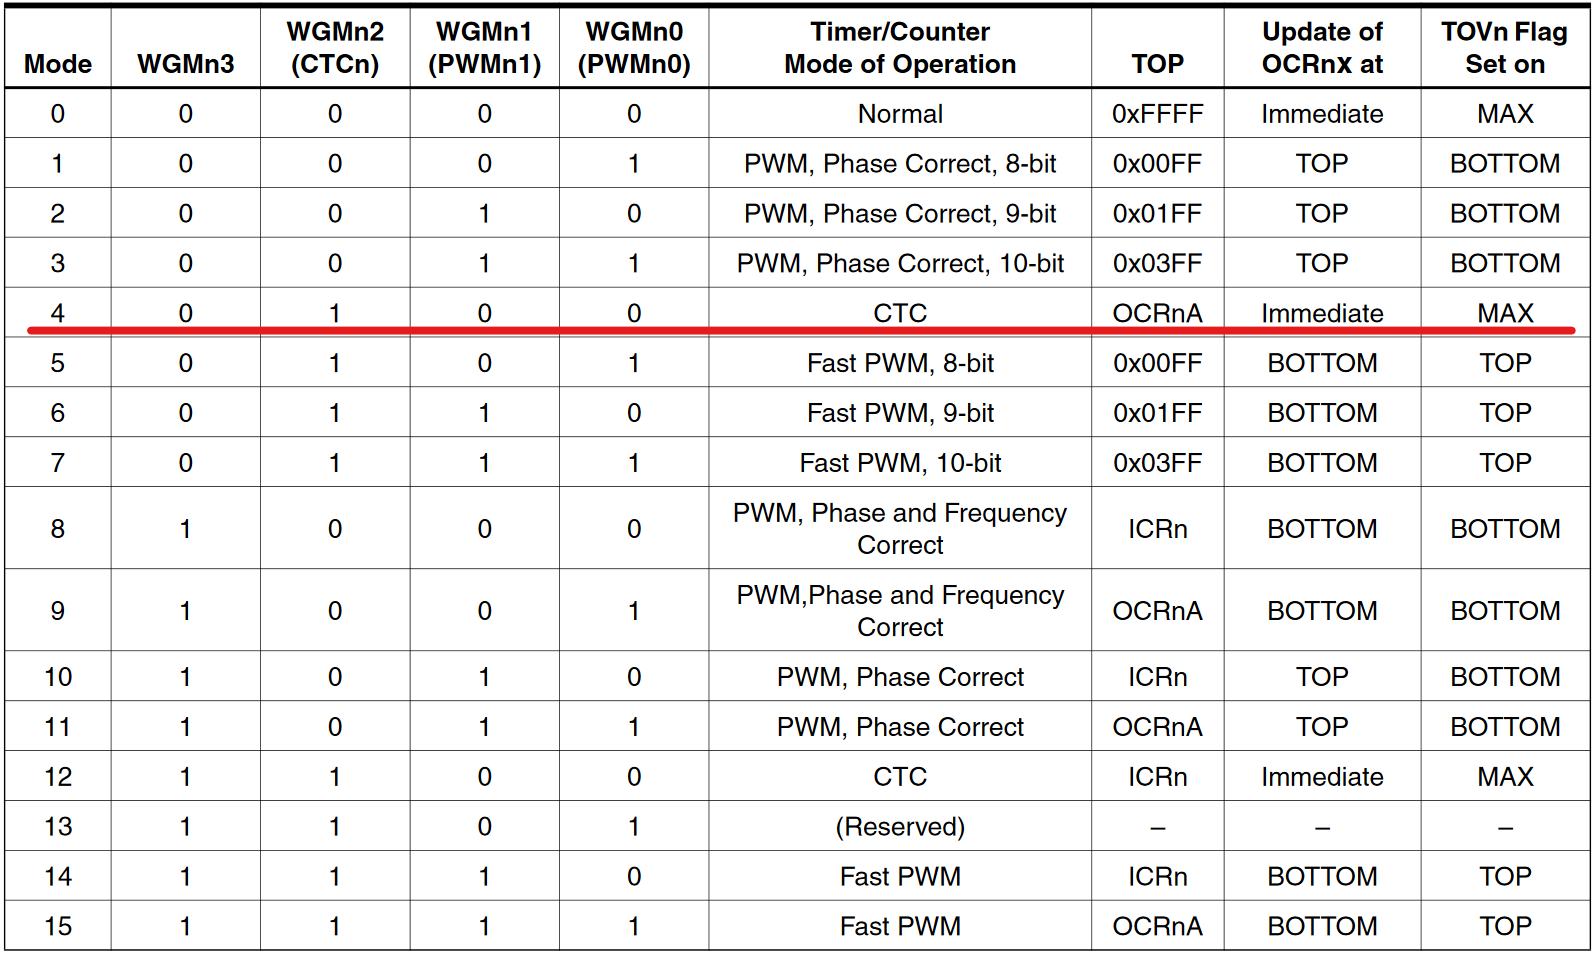
\includegraphics[width=\textwidth]{graphics/Timer_CTC_Mode}
	\caption{Timing-Diagramm CTC-Mode. OCnx nicht angeschlossen, Pin wird softwaremässig getoggelt.}
	\label{fig:Timer_CTC_Mode}
\end{figure}

\begin{figure}[h!]
	\centering
	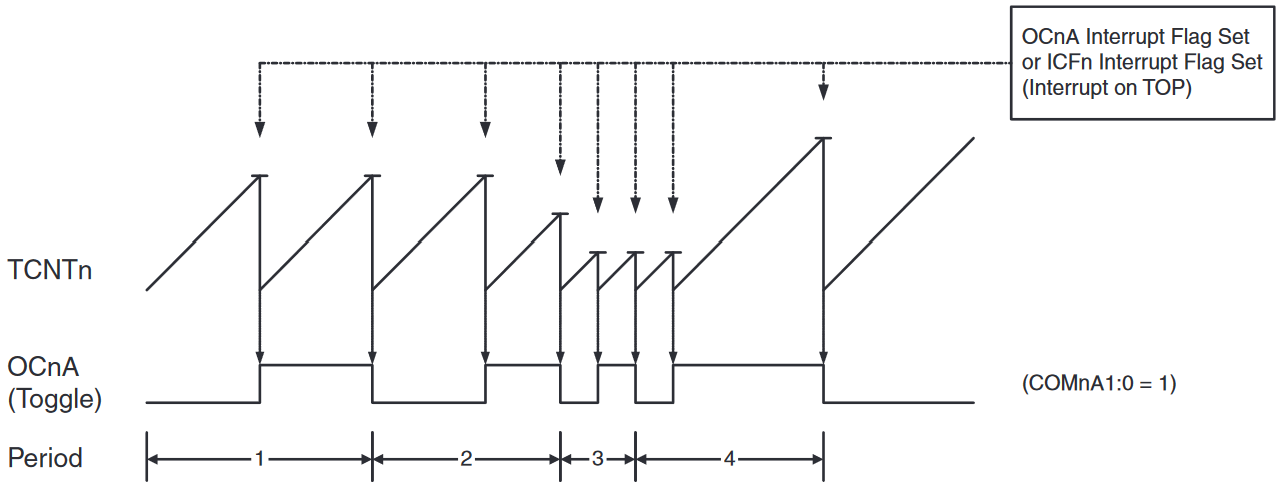
\includegraphics[width=\textwidth]{graphics/Timer_CTC_Timing_Diagram}
	\caption{Timing-Diagramm CTC-Mode. OCnx nicht angeschlossen, Pin wird softwaremässig getoggelt.}
	\label{fig:Timer_CTC_Timing_Diagram}
\end{figure}

\todo{cites: Atmel Datenblatt S.146}

Der Duty-Cycle wird Prozentual zum OCRnA-Register gesetzt. Wird für den berechneten Wert ein Duty-Cycle von 50\% vorgegeben, ergibt sich für das OCRnB-Register den Wert $(800 / 2) -1 \approx 399$. So wird nach der Hälfte der Hochzählzeit ein zweiter Compare-Interrupt ausgelöst, welcher jedoch kein Einfluss auf das Counter-Register hat.

Nun muss in beiden der erwähnten Interrupt-Routinen das gewünschte LED getoggelt werden. In der ersten Interruptroutine mit dem OCRnA-Compare-Register wird die LED eingeschaltet, in der zweiten Interruptroutine mit dem OCRnB-Compare-Register wird die LED ausgeschaltet.

Möchte man nun die Helligkeit angepasst werden, kann ein Wert zwischen 0 und OCRnA ausgewählt werden und damit das Register OCRnB beschrieben werden.

\todo{cite:  Formel - Atmega datenblatt S.121 }
\todo{cite:  Prescaler - Atmega datenblatt S.129 }
\todo{cite:  CTC-Mode - Atmega datenblatt S.145 }
\todo{cite:  CTC-Timing-Diagramm - Atmega datenblatt S.146 }

Der Wert für das OCRnA-Register ist folglich 799. Ein OCRnB-Register wird nicht benötigt, da die Iteration nur ausgeführt wird, sobald ein OCRnA-Compara-Match-Interrupt ausgelöst wird.

\subsubsection{Custom-Funktion}

Bei der Custom-Funktion können die Farbwerte manuell definiert werden. So wird für eine bestimmte Farbe für jede LED-Farbe der entsprechende Wert in das OCRnB-Register geschrieben. Darf sich eine Farbe nicht verändern, so muss das OCRnB-Register den gleichen Wert behalten. Die Itearation durch den Rainbow-Algorithmus wird im Custom-Mode nicht benötigt.

\subsubsection{Rainbow-Funktion}

Die Farbe der RGB-LED soll nun jeweils fünf Sekunden brauchen, um einen Farbteil komplett ein- oder auszuschalten, was einen sanften Übergang im Farbkreis ermöglicht.

Im Rainbow-Loop gibt es sechs States. Zubeginn muss die grüne LED schon voll leuchten.
\begin{enumerate}
\item Start ==> Grün
\item Hochzählen des Rot-Anteils ==> Yellow
\item Runterzählen des Grün-Anteils ==> Rot
\item Hochzählen des Blau-Anteils ==> Magenta
\item Runterzählen des Rot-Anteils ==> Blau
\item Hochzählen des Grün-Anteils ==> Cyan
\item Runterzählen des Blau-Anteils ==> Grün
\item Repeat 2 - 7
\end{enumerate}

Es benötigt 800 Schritte um einen Farbteil komplett ein- und auszuschalten. Pro Interrupt wird ein Schritt hochgezählt. Mit Formel \ref{equ:Milli_S} kann direkt berechnet werden, mit welchem Wert das Compare-Register beschrieben werden muss, sodass es fünf Sekunden geht, bis 800 Schritte hochgezählt wurden.

\begin{equation}
OCR_{nx} = \frac{f_{clk_{I/O}}}{2 \cdot N \cdot f_{OC_{max}}} - 1 = \frac{16MHz}{2 \cdot 1024 \cdot \frac{5s}{800 Schritte}} - 1 \approx 48
\label{equ:Milli_S}
\end{equation}

Die Iteration durch den Rainbow-Modus wird folglich mit einer Frequenz von 160Hz initialisiert. In der Routine wird demnach alle 6.25ms der Duty-Cytle einer Farbe hoch oder runtergezählt, und das Timer-Compare-Register des entsprechenden LED-Timers angepasst.

\subsubsection{Vorgehen}

\begin{enumerate}
\item Benötigte Applikation aus dem Software-Ordner auf dem USB-Stick in Atmel Studio öffnen.\\
\textcolor{magenta}{Software\textrightarrow Atmega\textrightarrow 3\underline{ }LED\underline{ }Control\textrightarrow 1\underline{ }LED\underline{ }Testsoftware\textrightarrow LED}\\

\item Software hochladen:\\
\textcolor{blue}{AtmelStudio\textrightarrow Tools\textrightarrow Cocktailmixer}\\

\end{enumerate}

\subsection{Motor}
\label{subsec:Inbetriebnahme_Motor}



\subsubsection{FOC-Treiber}
\label{subsubsec:Inbetriebnahme_FOC_Treiber}

Der FOC-Treiber wird über die SPI-Schnittstelle in Betrieb genommen. Dazu werden die Parameter verwendet, welche aus der TMCL-IDE verwendet werden. Die Standardparameter beinhalten Informationen zum Motor, zwei Sekunden Linksdrehung im Open-Loop, 2 Sekunden Rechtsdrehung im Open-Loop und dann Stop. Welche Register wie beschrieben werden, ist im Anhang Kapitel \ref{Appendix:TMC4671_Register} zu ersichtlich. Die Initialisierung sowie das Auslesen gewisser Register ist mit der Testapplikation ''\textit{3\underline{ }Motor\underline{ }Openloop}'' möglich, welche im Softwareordner auf dem USB-Stick zu finden ist.
\todo{Abgabe USB-Stick/Github-Account ??}
Das Setup, mit welchem der Treiber softwareseitig in Betrieb genommen wurde, ist im Anhang Kapitel \ref{Appendix:TMC4671_Setup} gezeigt.

Vorgehen:
\begin{enumerate}
\item Benötigte Applikation aus dem Software-Ordner auf dem USB-Stick in Atmel Studio öffnen.\\
\textcolor{magenta}{Software\textrightarrow Atmega\textrightarrow 3\underline{ }Motor\underline{ }Openloop\textrightarrow 1\underline{ }Motor\underline{ }Testsoftware\textrightarrow Motor}\\

\item Software anpassen: Zeile 23 bis 32\\
\textcolor{OliveGreen}{
	initTMC4671\underline{ }Openloop();\\
\\
    while (1) \\
    \{\\
		\underline{ }delay\underline{ }ms(10000);\\
		read\underline{ }registers\underline{ }TMC4671();\\
    \}
}\\

\item Software hochladen:\\
\textcolor{blue}{AtmelStudio\textrightarrow Tools\textrightarrow PartyMixer}\\

\item SPI-Kommunikation und ausgehende Gate-Signale vom FOC-Treiber zum Gate-Treiebr mit Oszilloskop überprüfen. Im Anhang Kapitel \ref{Appendix:TMC4671_SPI} sind die Messbilder zur SPI- Kommunikation zu finden und in Anhang \ref{Appendix:TMC4671_Gate_Ctrl} die Messbilder zur Gate-Control vom TMC4671 zum TMC6200.
\end{enumerate}

\todo{Skripts nicht benutzen in der Maschine.}

\subsubsection{Gate-Treiber, H-Brücke und BLDC}
\label{subsubsec:Inbetriebnahme_Gate_Treiber}

Der Gate-Treiber wird ebenfalls über die SPI-Schnittstelle in Betrieb genommen. Dazu werden die Parameter verwendet, welche in der TMCL-IDE verwendet wurden. Eine detaillierte Auflistung der beschriebenen Register ist im Anhang Kapitel \ref{Appendix:TMC6200_Register} zu finden. Mit den Standardparametern muss am Motoranschluss die selbe Signalfolge anliegen wie am sie auch am FOC-Treiber anliegen (Verstärkt durch H-Brücke). Die Initialisierung sowie das Auslesen gewisser Register ist mit der Testapplikation ''\textit{3\underline{ }Motor\underline{ }Openloop}'' möglich.

Das Setup, welches in Kapitel \ref{subsubsec:Inbetriebnahme_FOC_Treiber} erwähnt wurde, ist jetzt um einen Baustein erweitert worden und in Anhang Kapitel \ref{Appendix:TMC4671_Setup} ersichtlich.

Achtung, wenn die Scripts auf den Mikrocontroller des PartyMixers geladen werden ist darauf zu achten, dass die Achse des Motors frei beweglich ist und das Förderband nicht mit der Achse mitdreht, da ansonsten Schäden an der Maschine entstehen können. Es wird empfohlen die Scripts mit Mikrocontroller und EVAL-Boards zu testen.

Vorgehen:
\begin{enumerate}
\item Benötigte Applikation, welche im Software-Ordner auf dem USB-Stick oder Github \cite{aebi_projekt-6softwareatmega_2020} zu finden ist, in Atmel Studio öffnen.\\
\textcolor{magenta}{Software\textrightarrow Atmega\textrightarrow 3\underline{ }Motor\underline{ }Openloop\textrightarrow 1\underline{ }Motor\underline{ }Testsoftware\textrightarrow Motor}\\


\item Software anpassen:\\
\textcolor{OliveGreen}{
	initTMC6200;\\
	initTMC4671\underline{ }Openloop();\\
\\
    while (1) \\
    \{\\
		\underline{ }delay\underline{ }ms(5000);\\
		read\underline{ }registers\underline{ }TMC6200();\\
		\underline{ }delay\underline{ }ms(10000);\\
		read\underline{ }registers\underline{ }TMC4671();\\
    \}
}\newline
\item Software hochladen:\\
\textcolor{blue}{AtmelStudio\textrightarrow Tools\textrightarrow PartyMixer}\\

\item SPI-Kommunikation und Signale an der H-Brücke überprüfen. Im Anhang Kapitel \ref{Appendix:TMC6200_SPI} sind die Messbilder zur SPI-Kommunikation zu finden und in Anhang \ref{Appendix:TMC6200_Gate_Ctrl} die Bilder zur Gate-Ctrl vom Gate-Treiber zur H-Brücke.

\end{enumerate}

Bei der H-Brücke geht es darum, die Schaltsignale der MOSFETs zu überprüfen, bevor der Motor angeschlossen wird. Sind die Signale gut, kann der Motor angeschlossen werden.

Das Setup mit dem Motor ist im Anhang Kapitel \ref{Appendix:H_Bruecke_Setup} und die Messung der Schaltsignale im Anhang Kapitel \ref{Appendix:H_Bruecke_Schaltsignale} ersichtlich.

Wird jetzt der Motor angeschlossen, dreht sich dieser mit der vorgegebenen Geschwindigkeit.

\subsubsection{BLDC und H-Brücke}
\label{subsubsec:Inbetriebnahme_BLDC_und_H-Brücke}

Der Vorgang zur Inbetriebnahme der H-Brücke und des BLDC ist der Selbe, wie in Kapitel \ref{subsubsec:Inbetriebnahme_Gate_Treiber} beschrieben wurde. Bei der H-Brücke geht es darum, die Schaltsignale der MOSFETs zu überprüfen, bevor der Motor angeschlossen wird. Sind die Signale gut, kann der Motor angeschlossen werden.

Das Setup mit dem Motor ist im Anhang Kapitel \ref{Appendix:H_Bruecke_Setup} und die Schaltsignale im Anhang Kapitel \ref{Appendix:H_Bruecke_Schaltsignale} ersichtlich.

Wird jetzt der Motor angeschlossen, dreht sich dieser mit der vorgegebenen Geschwindigkeit.

\newpage
\subsubsection{ABN-Encoder}
\label{subsubsec:Inbetriebnahme_ABN-Encoder}

Der ABN-Encoder wird an den FOC-Treiber angeschlossen. Daher wird die Schnittstelle für den ABN-Encoder am TMC4671 initialisiert. Dazu werden die Parameter verwendet, welche in der TMCL-IDE verwendet wurden. Die zu schreibenden Parameter sind im Anhang Kapitel \ref{Appendix:ABN_Register} angehängt. Das Einlesen der PWM-Signale wird getestet, indem der Treiber in den Positionsmodus versetzt wird, wozu das Feedback des Rotors nötig ist. Hat die Initialisierung funktioniert, dreht sich der Motor an eine gewünschte Position und haltet dort. Zur Initialisierung gehören auch einige Einstellungen zu den PI-Reglern. Die Initialisierung sowie das Auslesen gewisser Register ist mit der Testapplikation ''\textit{4\underline{ }Motor\underline{ }ABN\underline{ }Encoder}'' möglich.

Die Regler, welche im FOC-Treiber integriert sind, werden verwendet, um einen Motor ein bestimmtes Drehmoment vorzugeben, ihn mit einer bestimmten Drehzahl drehen zu lassen und/oder ihn an eine bestimmte Position zu fahren. Im Gegensatz zu einem Motor, welchem nur eine Spannung vorgegeben wird, kann bei diesem Regelverfahren bei einer Abweichung des vorgegebenen Parameters nachgeregelt werden. So kann beispielsweise bei grösserer Belastung die angelegte Spannung erhöht werden, sodass die vorgegebene Geschwindigkeit gehalten werden kann.

Die Regelung eines Motors kann verschieden aufgebaut sein. Die Regelstruktur, wie sie im FOC-Treiber TMC4671 integriert ist, ist eine Kaskadenregelung. Eine Kaskadenregelung besteht in der Regel aus drei überlagerten Regelkreisen. Der innerste Regelkreis ist der Stromregelkreis. Dieser ist dem Geschwindigkeitsregelkreis unterlagert. Der Geschwindigkeitsregelkreis ist wiederum dem Positionsregelkreis unterlagert. Bei einer Kaskadenregelung ist die Ausgangsgrösse des überlagerten Regelkreises die Eingangsgrösse des unterlagerten Regelkreises. Aus Stabilitätsgründen ist darauf zu achten, dass die Nachstellzeit der äusseren Regelkreise grösser ist, als die der Inneren.


Die Regelung im TMC4671 besteht im innersten aus einem schnellen Stromregelkreis. Dieser soll in der Lage sein, schnellst möglich auf eine Abweichung des vorgegebenen Drehmoments zu reagieren. Die Abweichung des Stromregelkreises ist ein wichtiger Parameter zur Berechnung des Modulationsindex, welcher der Kommutierung des Motors dient.

Der Geschwindigkeitsregelkreis ist dem Stromregelkreis überlagert. Weicht die aktuelle Geschwindigkeit von der vorgegebenen Geschwindigkeit ab, so gibt der Geschwindigkeitsregelkreis dem Stromregelkreis eine Abweichung vor, wodurch der Strom durch die Spulen und somit das Drehmoment erhöht oder gesenkt wird.

Der Positionsregelkreis ist dem Geschwindigkeitskreis überlagert. Weicht die aktuelle Position von der vorgegebenen Position ab, so gibt der Positionsregelkreis dem Geschwindigkeitsregelkreis eine Abweichung vor, wodurch der Geschwindigkeitsregelkreis in die erforderliche Richtung korrigiert.

Mit der Begrenzung der Eingangsgrössen wird die Mechanik geschont und der Motor vor Überlast geschützt. Dies wird erreicht, indem die Ausgangsgrössen der PI-Regler mit einem Limit versehen werden. So kann der Strom durch die Spulen begrenzt werden, eine Maximalgeschwindigkeit definiert werden und die Enden der Positionen vorgegeben werden. Die Limits sind auf den Motor abgestimmt. \cite{stahl_simulation_2014}

Die Werte der PI-Regler wurden Experimentell bestimmt. Folgende Werte wurden dabei ermittelt:

\begin{tabularx}{\linewidth}{|l|X|X|l|}
\hline
\textbf{Regelkreis} & \textbf{P-Anteil} & \textbf{I-Anteil} & \textbf{Nachstellzeit}\\
\hline
Drehmoment & 100 & 1200 & \\
\hline
Fluss & 100 & 1200 & \\
\hline
Geschwindigkeit & 2000 & 300 & \\
\hline
Position & 100 & 0 & \\
\hline
\end{tabularx}

\todo{Nachstellzeit?}

Die Limits wurden folgendermassen gesetzt:

\begin{tabularx}{\linewidth}{|l|X||l|X|}
\hline
\textbf{Limit} & \textbf{Wert} & \textbf{Limit} & \textbf{Wert}\\
\hline
Drehmoment & 2500 & Fluss & 2500\\
\hline
Geschwindigkeit & 1500 &  & \\
\hline
\end{tabularx}

Die Regler wurden so bestimmt, dass die Regelkreise in unbelasteten Zustand ihre Sollwerte schnellst möglich erreichen, ohne überzuschiessen. Dies betrifft den Regler für den Stromregelkreis und den Regler für den Geschwindigkeitsregelkreis. Die zugehörigen Parameter wurden in der TMCL-IDE ermittelt. 

Das bisherige Setup hat sich nun um den ABN-Encoder erweitert und ist im Anhang Kapitel \ref{Appendix:ABN_Setup} ersichtlich.

Vorgehen:
\begin{enumerate}
\item Benötigte Applikation aus dem Software-Ordner auf dem USB-Stick in Atmel Studio öffnen.\\
\textcolor{magenta}{Software\textrightarrow Atmega\textrightarrow 4\underline{ }Motor\underline{ }ABN\underline{ }Encoder\textrightarrow 1\underline{ }Motor\underline{ }Testsoftware\textrightarrow Motor}\\

\item Software hochladen:\\
\textcolor{blue}{AtmelStudio\textrightarrow Tools\textrightarrow PartyMixer}\\

\item Ausgehende Signale des ABN-Encoders überprüfen. Im Anhang Kapitel \ref{Appendix:ABN_Signale} ist das Messbild des ABN-Encoder-Ausgangs zu sehen.

\end{enumerate}

\subsubsection{PI-Regler}
\label{subsubsec:PI_Regler}

Die Regler, welche im FOC-Treiber integriert sind, werden verwendet, um einen Motor an eine bestimmte Position zu fahren, mit einer bestimmte Geschwindigkeit drehen oder ein bestimmtes Drehmoment anzulegen. Im Gegensatz zu einem Motor, dem nur eine Spannung vorgegeben wird, kann bei einer Abweichung des vorgegebenen Parameters nachgeregelt werden. So kann beispielsweise bei grösserer Belastung die angelegte Spannung erhöht werden, sodass die vorgegebene Geschwindigkeit gehalten werden kann.

Für die Regelung eines Motors können verschieden aufgebaut sein. Die Regelstruktur, wie sie im FOC-Treiber TMC4671 integriert ist, ist eine Kaskadenregelung. Eine Kaskadenregelung besteht in der Regel aus drei überlagerten Regelkreisen. Der innerste Regelkreis ist der Stromregelkreis. Dieser ist dem Geschwindigkeitsregelkreis unterlagert. Der Geschwindigkeitsregelkreis ist wiederum den Positionsregelkreis unterlagert. Bei einer Kaskadenregelung ist die Ausgangsgrösse des überlagerten Regelkreises die Eingangsgrösse des unterlagerten Regelkreises. Aus stabilitätsgründen ist darauf zu achten, dass die Nachstellzeit der äusseren Regelkreise grösser ist, alsi die der Inneren.

Die Regelung im TMC4671 besteht aus einem innersten, schnellen Stromregelkreis. Dieser soll in der Lage sein, schnellst möglich mit einer Erhöhung des Drehmomentes auf eine Abweichung zu reagieren. Ausserdem gibt der Stromregelkreis die Kommutierung des Motors vor.

Der Geschwindigkeitsregelkreis ist dem Stromregelkreis überlagert. Weicht die aktuelle Geschwindigkeit von der vorgegebenen Geschwindigkeit ab, so gibt der Geschwindigkeitsregelkreis dem Stromregelkreis eine Abweichung vor, wodurch der Strom durch die Spulen und somit das Drehmoment erhöht oder gesenkt wird.

Der Positionsregelkreis ist dem Geschwindigkeitskreis überlagert. Weicht die aktuelle Position von der vorgegebenen Position ab, so gibt der Positionsregelkreis dem Geschwindigkeitsregelkreis eine Abweichung vor, wodurch der Geschwindigkeitsregelkreis in die erforderliche Richtung korrigiert.

Mit der Begrenzung der Eingangsgrössen wird die Mechanik geschont und der Motor vor Überlast geschützt. Dies wird erreicht, indem die Ausgangsgrössen der PI-Regler mit einem Limit versehen werden. So kann der Strom durch die Spulen begrenzt werden, eine Maximalgeschwindigkeit definiert werden und die Enden der Positionen vorgegeben werden. Die Limits sind auf den Motor abgestimmt. \cite{stahl_simulation_2014}

Die Werte der PI-Regler wurden Experimentell bestimmt. Folgende Werte wurden dabei ermittelt:

\begin{tabularx}{\linewidth}{|l|X|X|l|}
\hline
\textbf{Regelkreis} & \textbf{P-Anteil} & \textbf{I-Anteil} & \textbf{Nachstellzeit}\\
\hline
Drehmoment & 100 & 1200 & \\
\hline
Fluss & 100 & 1200 & \\
\hline
Geschwindigkeit & 2000 & 300 & \\
\hline
Position & 100 & 0 & \\
\hline
\end{tabularx}

Die Limits wurden folgendermassen gesetzt:

\begin{tabularx}{\linewidth}{|l|X||l|X|}
\hline
\textbf{Limit} & \textbf{Wert} & \textbf{Limit} & \textbf{Wert}\\
\hline
Drehmoment & 2500 & Fluss & 2500\\
\hline
Geschwindigkeit & 1500 &  & \\
\hline
\end{tabularx}

Die Regler wurden so bestimmt, dass die Regelkreise in unbelasteten Zustand ihre Sollwerte schnellst möglich erreichen, ohne überzuschiessen. Dies Betrifft den Regler für den Stromregelkreis und den Regler für den Geschwindigkeitsregelkreis. Die zugehörigen Parameter wurden in der TMCL-IDE ermittelt. 

Mit diesen Werte ist es nur schwierig realisierbar, den Schlitten mit einer kontrollierten Bewegung fortzubewegen. Um dennoch gezielt Positionen anzufahren, wurde eine Software-Ramp geschrieben. Diese berechnet den gewünschten Weg unter Berücksichtigung der maximalen Beschleunigung und der maximalen Geschwindigkeit. Durch eine periodische Iteration in Millisekunden-Schritten über die Zeit gibt die Ramp dem FOC-Treiber schrittweise die berechnete Position vor. Die Endposition, die Geschwindigkeit und die Beschleunigung der Ramp sind einfach skallierbar, was eine schnellere Einbettung in das Gesamtsystem ermöglicht.

\newpage
\section{Software}
\label{sec:Software}



\subsection{Atmega2560}
\label{subsec:Software_Atmega2560}

Die Software für den Atmega2560 ist wie folgt aufgebaut: 
Im \textbf{Init/Main} werden die Variablen deklariert, welche im Programm benutzt werden, um die aus den Kommunikationsbuffern geholten Daten zur Verarbeitung zu Speichern.
Zudem werden hier die Adressen auf die Funktionen deklariert, welche die Module (z.B IO, Speicher, Devices, Interfaces) initialisieren und die Buffer in der main-Schleife prüfen.
Durch Aufrufen des h-Files ''Cocktail\_Statemachine.h'' werden die Adressen der projektspezifischen Funktionen deklariert und somit die \textbf{User-Applikation} eingebunden. Darunter befinden sich die Libraries, welche die Registernummern oder Befehlssätze beinhalten, um die Devices anzusteuern.
Sie bilden die Schnittstelle zwischen User-Applikation und Kommunikationsinterface.
Dies ist vergleichbar mit einem \textbf{Application-Programming-Interface}\footnote{API, Schnittstelle zur Anwendungsprogrammierung}, einem Programmteil, welcher eine Verbindung eines Programms zu einem anderen Programm ermöglicht. 
Die Informationen werden dabei standardisiert zwischen den Anwendungen ausgetauscht.
Die Daten oder Befehle werden strukturiert nach einem definierten Syntax übergeben.
Der Zugriff auf die Hardware des Mikrocontrollers (SPI- und UART-Interface) erfolgt mittels den AVR-Registern.
Die Libraries, die dafür verwendet werden befinden sich folglich zwischen dem ''API''-Layer und der Hardware und können mit der \textbf{Hardware Abstraction Layer}\footnote{HAL, Hardwareabstraktionsschicht} verglichen werden.
Es wird nur über diese Funktionen auf die entsprechende Hardware zugegriffen. \cite{geisler_was_2018}


\subsubsection{Strukturplan}
\label{subsubsec:Strukturplan_Atmega}

In Abbildung \ref{fig:Softwareuebersicht_Atmega2560} wird aufgezeigt, wie die Software aufgebaut ist und welcher Teil der Software von welchen Libraries abhängig ist. Wie in Kapitel \ref{subsec:Software_Atmega2560} beschrieben kann die Software in folgende Teile gegliedert werden:
\begin{itemize}
\item Init/Main
\item User Application
\item API - Application-Programming-Interface
\item HAL - Hardware-Abstraction-Layer
\item Interfaces / Pins
\end{itemize}

\begin{figure}[h!]
	\centering
	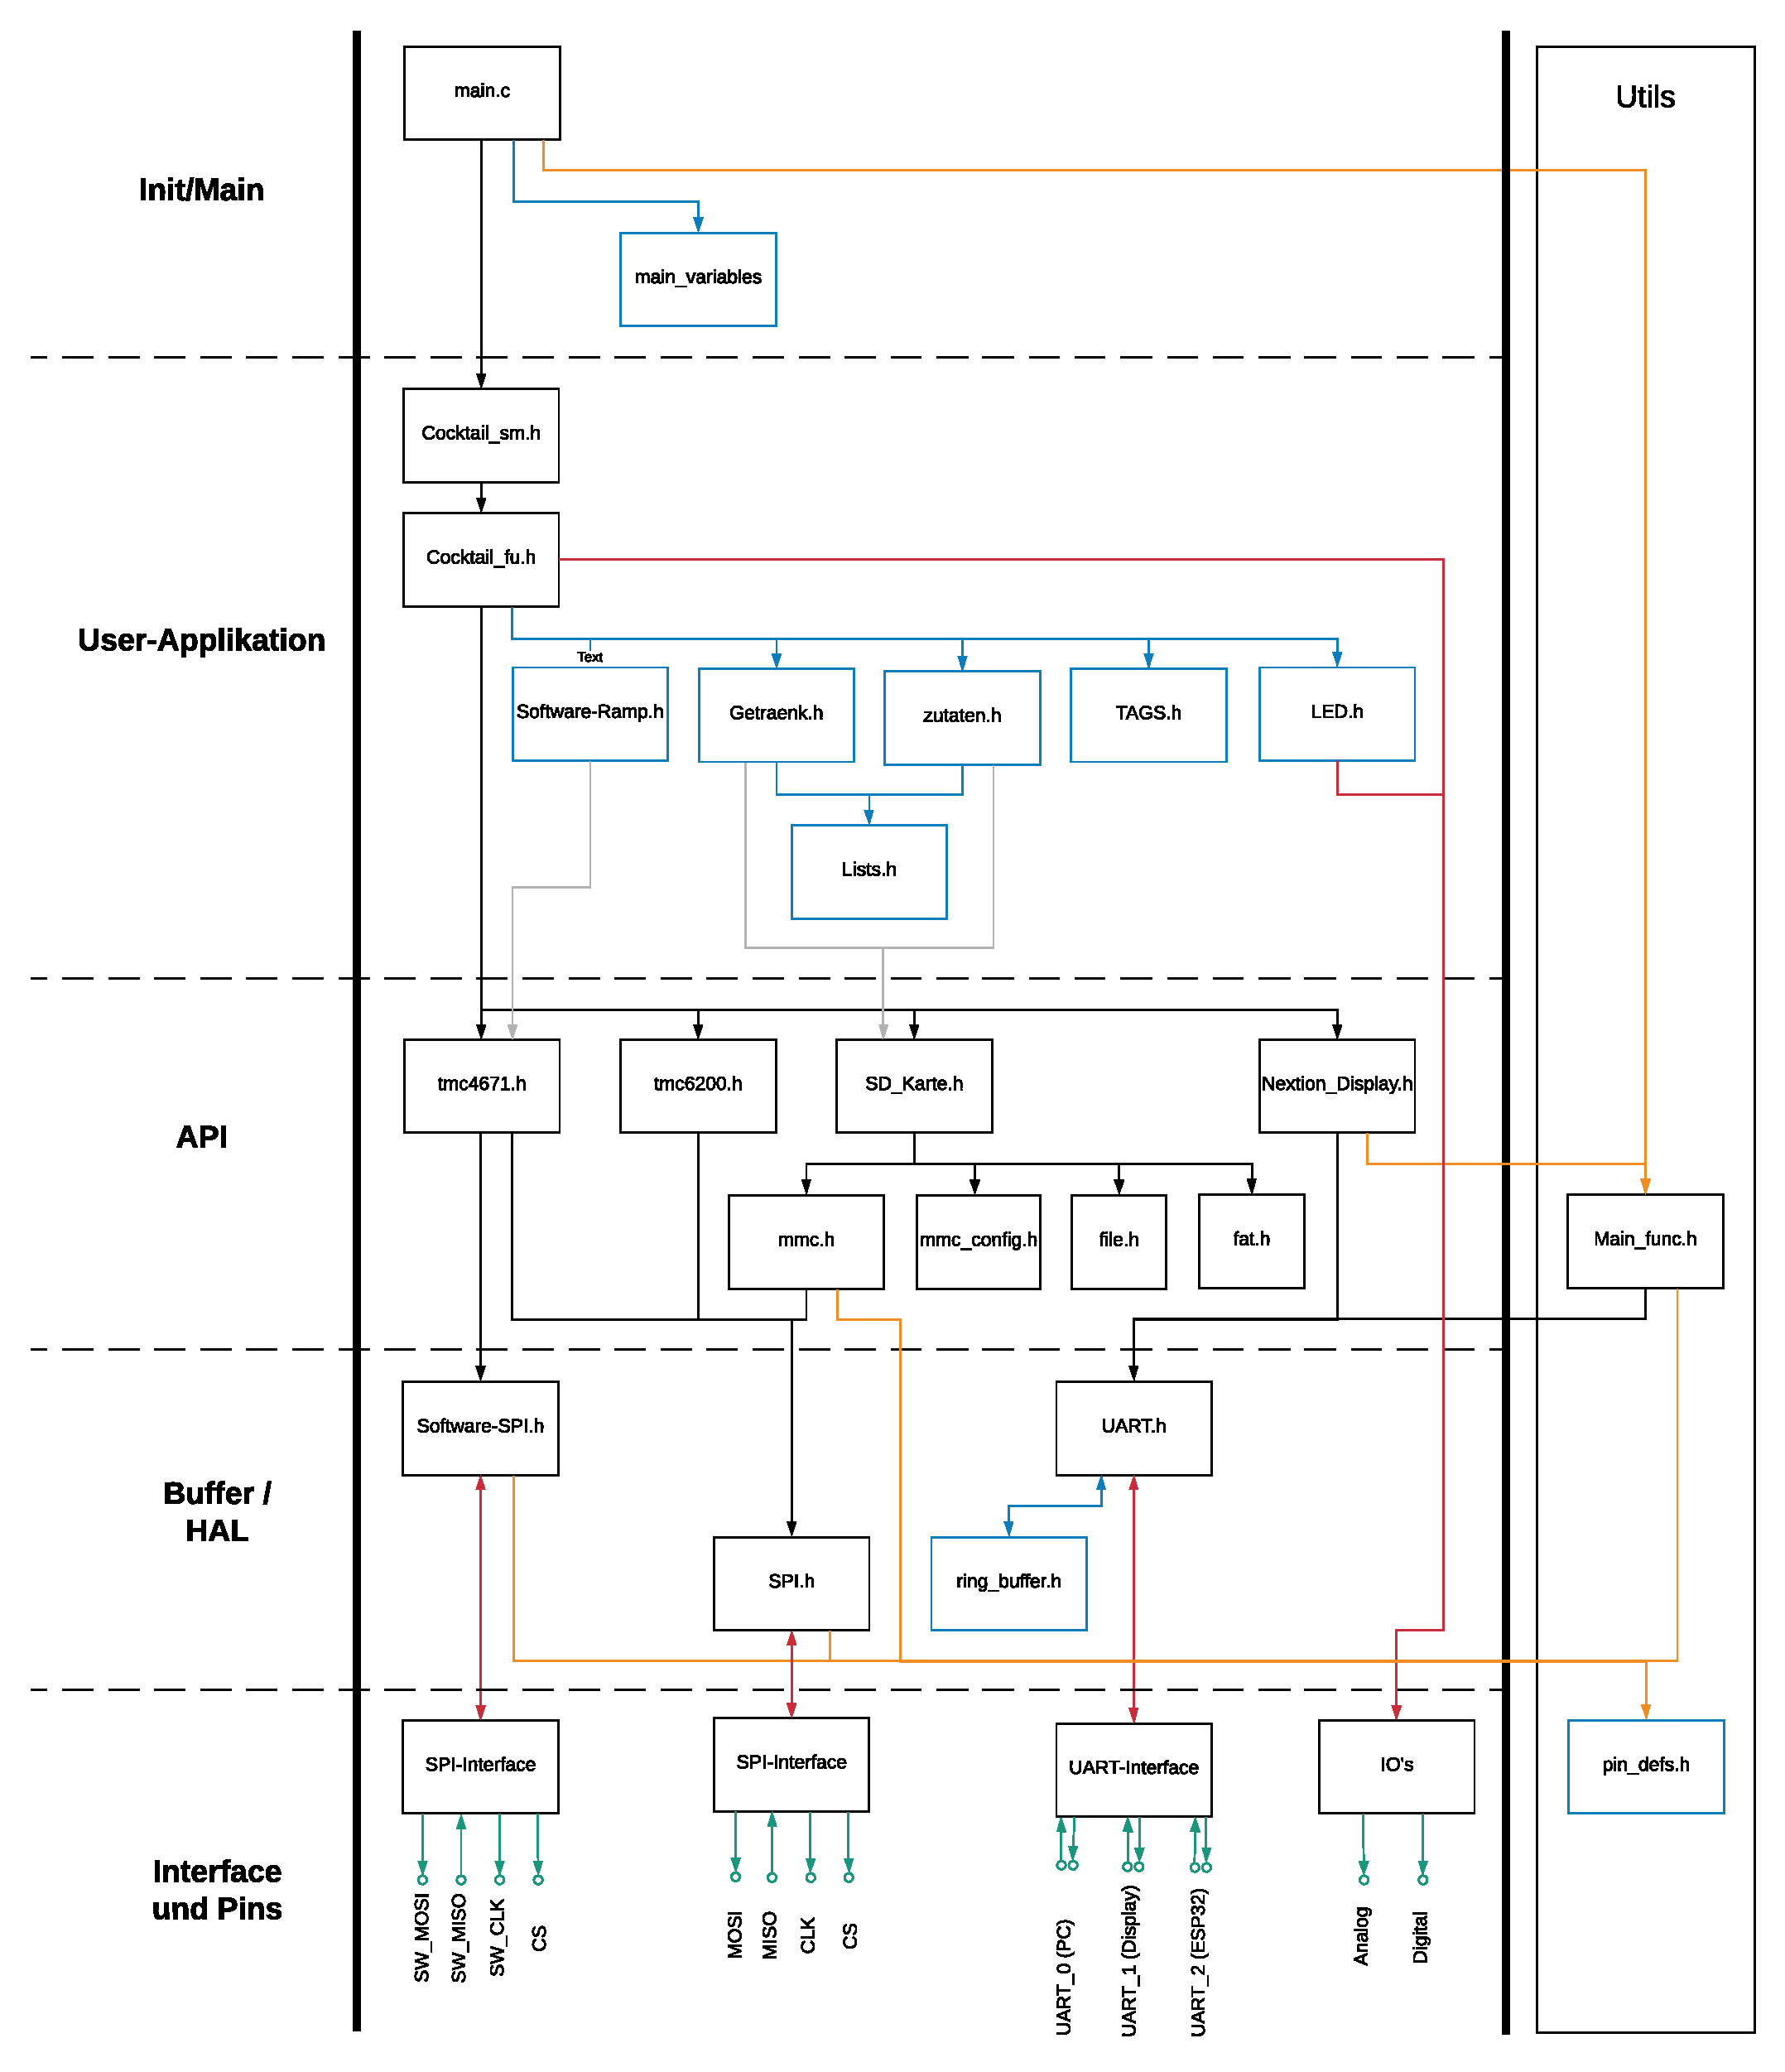
\includegraphics[width=\textwidth]{graphics/Softwareuebersicht.pdf}
	\caption{Softwareübersicht Atmega2560.}
	\label{fig:Softwareuebersicht_Atmega2560}
\end{figure}



\subsubsection{Programmflussdiagramm}
\label{subsubsec:Programmflussdiagramm}

\paragraph{Bootloader-Section}\mbox{}\\
In Abbildung \ref{fig:Programmfluss_Atmega2560} wird der Programmfluss der Atmega2560-Software aufgezeigt. Beim einschalten des Mikrocontrollers wird in der Bootloader-Section zuerst der Bootloader gestartet (Boot Loader Flash Section). Sofern keine neue Software über die UART0-Schnittstelle kommt, so beginnt das Cocktail spezifische Programm (Application Flash Section). Sofern eine neue Software über die UART0-Schnittstelle gesendet wird, wird die kommende Software in diese Application Flash Section geschrieben und das Programm nach der Übertragung gestartet.

\paragraph{Init-Section}\mbox{}\\
Wird das Programm gestartet, beginnt die Init-Section. Hier werden die zuerst die Main-Variablen initialisiert. Danach werden die Adressen der Funktionen ins Programm geladen mittels den h-Files. Die Interfaces (SPI, Uart, I/O's) müssen als erstes initialisiert werden, damit die Initialisierung der SPI-Devices stattfinden kann und Boot-Informationen über eine gewünschte Schnittstelle angezeigt werden können (z.B Uart0 ==> Computer). Sobald die Schnittstellen initialisiert wurden, werden die Devices initialisiert. Dazu gehören die SD-Karte, der FOC-Treiber und der Gate-Treiber. Daraufhin werden die Speicher-Strukturen initialisiert, welche für die User-Applikation (Tabelle \ref{fig:Softwareuebersicht_Atmega2560} in Kapitel \ref{subsubsec:Strukturplan_Atmega}) gebraucht werden. Die Struktur und Anwendung der Speicherplätze wird in Kapitel \ref{Appendix:Lists} erklärt. Zu guter Letzt wird die Startanzeige des Displays geladen.

\paragraph{Main-Loop}\mbox{}\\
Da die Maschine nur auf Inputs reagieren muss, werden im Main-Loop nur die Buffer der Devices abgefragt. Sobald ein Terminator-Zeichen ankommt (z.B ein carriage return '\textbackslash r' der UART0-Schnitstelle oder 0xFF 0xFF 0xFF der UART1-Schnittstelle), werden die zuvor empfangenen Daten interpretiert und verarbeitet.

\newpage

\begin{figure}[h!]
	\centering
	\includegraphics[width=0.6\textwidth]{graphics/Programmfluss_Atmega2560.pdf}
	\caption{Programflussdiagramm Atmega2560.}
	\label{fig:Programmfluss_Atmega2560}
\end{figure}
\newpage


\subsubsection{Speicherorganisation}\label{subsubsec:Speicherorganisation}

Da im Programmfluss viel mit Listen gearbeitet wird, wird auf \textit{Doubly Dynamic Linked Lists} zurückgegriffen.
Eine Doppelt verkettete Liste ist eine gängige Datenstruktur, um sich einfach und effizient in einer Liste hoch und runter zu bewegen. Weiter können der Liste ohne grossen Aufwand sogenannte Nodes\footnote{Nodes = Knoten} hinzugefügt werden. Im Folgenden wird von Elementen statt von Nodes gesprochen. Für jedes Element werden zwei Pointer initialisiert, welche auf das nächste (next) oder auf das vorherige (prev) Element zeigen. Nebst den Zeigern auf die umliegenden Elemente enthält das Element die gewünschten Daten. Um zu wissen, ob das Ende oder der Beginn erreicht wurde, werden zwei zusätzliche Zeiger initialisiert, welche auf das erste und/oder letzte Element zeigen (Head und Tail). Im Anhang Kapitel \ref{Appendix:Lists} können weitere Details zu Dynamic Linked Lists entnommen werden.\cite{lenz_artikel_2016}

Abbildung \ref{fig:Doubly_Linked_List_2_00} zeigt eine Struktur der beschriebenen Liste mit next, prev, head, tail und Elementen.

\begin{figure}[h!]
	\centering
	\includegraphics[width=0.5\textwidth]{graphics/Doubly_Linked_List_2_00}
	\caption{Doppelt verkettete Liste mit zwei Elementen.\cite{yadav_circular_2019}}
	\label{fig:Doubly_Linked_List_2_00}
\end{figure}


Die Elemente sind in Structs organisiert, welche die Zeiger und die Daten enthalten. In der Software werden verschiedene Struct-Typen verwendet. Für jeden Struct-Typ lässt sich eine Liste mit mehreren Structs erstellen. Es werden für die folgenden vier Elemente Listen angelegt:

\begin{itemize}
\item Cocktail-Liste (SD-Files)
\item Zutaten-Liste (SD-Files)
\item Tag-Liste (Maschine)
\item Zutaten-in-Maschine-Liste (Maschine)
\end{itemize}

Da während der Entwicklung der Programmspeicher mit zu vielen Daten gefüllt wurde, stürzte der Mikrocontroller ab. Die Cocktail- und die Zutaten-Liste beinhalten deshalb nur die Nummer ein zugehöriges Files, welches sich auf der SD-Karte befindet. Wird ein Cocktail oder eine Zutat benötigt, so werden die Daten temporär von der SD-Karte in einen Struct im Programmspeicher geladen und verschwinden wieder, sobald ein neues Element geladen wird.

Die Tag-Liste sowie die Liste der Zutaten in der Maschine werden komplett in den Programmspeicher geladen. Die beiden Listen werden bei einer Veränderung als Backup jeweils in einem File gespeichert, damit diese bei einem Neustart der Maschine wieder in den Programmspeicher geladen werden können.

\subsection{ESP32}
\label{subsec:Software_ESP32}

Bei der Inbetriebnahme in Kapitel \ref{subsubsec:ESP} wurde das ESP32 mittels eines Web-Servers getestet und in Betrieb genommen. Da jedoch dies für einen Benutzer relativ umständlich ist, wurde eine Android-App erstellt, mit welcher Befehle an das ESP32 gesendet werden können. Diese kommuniziert über Bluetooth und hat den Vorteil, dass eine App einiges Benutzerfreundlicher ist, da App's im Alltag fast jeder Person integriert sind. \cite{santos_esp32_2018}  

Die Software für das ESP32 wurde komplett in Arduino IDE geschriben und beinhaltet folgende Bereiche:

\begin{itemize}
\item Daten von der App empfangen
\item Daten an die App senden
\item Daten vom uP abfragen
\item Daten an den uP senden 
\item Daten vom RFID-Leser empfangen
\end{itemize}

Im Programm werden zuerst die notwendigen Bibliotheken  eingebunden. Dabei werden folgende Bibliotheken verwendet:

\begin{itemize}
\item Arduino.h
\item BluetoothSerial.h
\item SPI.h
\item MFRC522.h
\end{itemize}

Dabei beinhaltet die \flqq Arduino.h\frqq~Bibliothek die Standardbefehle von Arduino, die \flqq BluetoothSerial.h\frqq~Bibliothek beinhaltet alle Kommunikationsbefehle um über Bluetooth kommunizieren zu können, die \flqq SPI.h\frqq~Bibliothek beinhaltet alle Kommunikationsbefehle um über SPI kommunizieren zu können und die \flqq MFRC522.h\frqq~Bibliothek beinhaltet alle Befehle um mit dem RFID-Modul arbeiten zu können.

Es wurde bei der Programmierung darauf geachtet, dass mit möglichst einfachen mitteln gearbeitet wird. Um zu Kommunizieren wurden die Datentypen String und char verwendet. Für Zählvariablen wurde der Datentyp int verwendet. 

\subsubsection{Programmflussdiagramm}
\label{subsubsec:Software_ESP32_Programmflussdiagramm}

\todo{Programmflussdiagramm} 
\todo{lucidchart.com}

\subsection{Displaysoftware}
\label{subsec:Software_Display}

Das NX8048T070 7-Zoll Display von Nextion wurde mit der dazugehörigen Software \flqq Nextion Editor\frqq~programmiert. Diese wurde eigens für die angebotenen Displaytypen entwickelt und erleichtern dem Benutzer die Erstellung von grafischen Oberflächen und deren Funktionen. Die Softwareoberfläche ist in Abbildung \ref{fig:NextionEditor} zu sehen. Der Aufbau ist simpel gestaltet. In der Mitte der Software befindet sich eine grosse Ansicht der bereits erstellten Displayseite. Darauf sind alle Komponenten zu sehen, welche schon platziert wurden und deren Formatierung. Auf der linken Seite können im oberen Bereich Elemente per Drag and Drop in die Displayseite gezogen werden. Unterhalb der Elementauswahl befindet sich ein Medienfenster, in welchem Bilder für Hintergründe der Elemente, Audiodateien und andere Medien abgespeichert werden können. Auf der rechten Seite im oberen Bereich befindet sich die Seitenansicht, worin alle erstellen Displayseiten sichtbar sind. Die ausgewählte Displayseite erscheint in der Mitte der Software. Um die gewählten Elemente formatieren zu können, befindet sich im unteren Bereich der rechten Seite ein Fenster mit den möglichen Formatierungen des jeweils gewählten Elementes. Unter der Displayseite gibt es noch ein Output-Fenster und ein Event-Fenster, in welchem die gewünschte Programmierung festgelegt werden kann. Ein cooles Feature des Nextion Editor's ist der Debug-Modus. Mit diesem Tool kann auch ohne Bildschirm die Funktion getestet werden. \cite{patrick_nx8048t070_nodate} \cite{zhou_nextion_nodate}

\begin{figure}[h!]
	\centering
	\includegraphics[width=\textwidth]{graphics/NextionEditor}
	\caption{Programmieroberfläche von Nextion \cite{zhou_nextion_nodate} \cite{pngimgcom_cocktail_nodate-7}}
	\label{fig:NextionEditor}
\end{figure}

\newpage
 




\subsubsection{Displaymenu}
\label{subsubsec:Software_Displaymenu}

Das Bedienmenü am Display bietet dem Benutzer viele Freiheiten, was ein umfangreiches und möglichst intuitives Bedienkonzept erforderte. Folgende Einstellungen und Anpassungen können vom Benutzer vorgenommen werden:


\begin{itemize}
\item Getränkeauswahl gemäss Bild oder Listenansicht
\item Zutatenabfrage
\item Bearbeitung von bereits existierenden Cocktails
\item Erstellen neuer Cocktails 
\item Individuelle Zusammenstellung und Positionierung von Flüssigkeiten
\item Zuweisung eines Getränkes zu einem RFID-Tag
\item Anzeige einer Maschineninfo
\item individuelle Beleuchtung der Maschine
\item Maschinen Reinigungsmodus
\end{itemize}

Im folgenden wird auf die gesamte Menüstruktur eingegangen und erklärt, wie diese zu bedienen ist.

\textbf{Hauptansicht}\\
In der Hauptansicht gemäss Abbildung \ref{fig:DisplayHauptmenu} wird die Getränkeauswahl getroffen. Dabei gibt es zwei verschiedene Auswahlmöglichkeiten. Mit den Pfeiltasten nach links oder rechts kann ein Getränk aus der Maschine ausgewählt werden. Es wird dabei immer der Getränkename und eine dazugehörige Abbildung angezeigt, damit dem Kunden der Cocktail auch schmackhaft gemacht werden kann. Will man schneller suchen, so kann man mittels \flqq Liste\frqq~eine Listenansicht öffnen, wobei man mit den Pfeiltasten nach oben und unten scrollen und den gewünschten Cocktail auswählen kann. Wird eine Auswahl getroffen, so gelangt man zurück in die Hauptansicht und der gewählte Cocktail erscheint mit dem dazugehörigen Bild. Mit \flqq Zurück\frqq~gelangt man ebenfalls zurück in die Hautansicht. Es gibt auch Filtermöglichkeiten. Auf der rechten unteren Seite des Display's kann per Klick entschieden werden, ob nur alkoholische, alkoholfreie oder alle Cocktails angezeigt werden. Hat man ein Getränk gefunden und möchte wissen was sich darin befindet und wie viel, so kann man mittels Klick auf \flqq Zutaten\frqq~ein Fenster öffnen, welches einem anzeigt was und wie viel davon sich darin befindet. Möchte man Einstellungen vornehmen, so gelangt man mittels \flqq Menü\frqq~in das Maschinenmenü.

\begin{figure}[H]
	\centering
	\includegraphics[width=\textwidth]{graphics/DisplayHauptmenu}
	\caption{Hauptansicht der Menüstruktur des Display's \cite{pngimgcom_cocktail_nodate-6}}
	\label{fig:DisplayHauptmenu}
\end{figure}

\textbf{Getränkeauslösung}\\
Wurde die Auswahl für ein Getränk getroffen, so kann man mittels Klick auf das Bild das Getränk auslösen. Dabei gelangt man in eine Abfrage, welche dem Kunden die Wahl lässt, ob er gerne 3dl oder 5dl haben möchte. Mit \flqq Abbrechen\frqq~gelangt man in die Hauptanzeige zurück. Bei Klick auf den entsprechenden Button 3dl oder 5dl wird die gewünschte Grösse des Getränks ausgelöst und am Bildschirm erscheint ein kleiner Text, welcher einem das Warten versüsst. Dazu muss natürlich ein Glas vom Kunden auf den Schlitten gelegt werden. Der Schlitten befördert nun das Glas zu den einzelnen Positionen und füllt es dort ab. Sobald das Getränk fertig ist, fährt der Schlitten an die Ausgangsposition zurück und es wird am Bildschirm angezeigt, dass das Getränk nun fertig ist. Es erscheint danach erneut der Hauptbildschirm und es kann von neuem gestartet werden. Wird während des Erstellungsvorgangs auf \flqq Abbrechen\frqq~gedrückt, so wird der Prozess abgebrochen und das Display zeigt dies an. In Abbildung \ref{fig:DisplayAusloesen} sind die dazugehörigen Bildschirme zu sehen.

\begin{figure}[H]
	\centering
	\includegraphics[width=\textwidth]{graphics/DisplayAusloesen}
	\caption{Auslösevorgang der Menüstruktur des Display's \cite{pngimgcom_cocktail_nodate-6}}
	\label{fig:DisplayAusloesen}
\end{figure}

\newpage

\textbf{Maschineninfo und LED-Beleuchtung}\\
Im Maschinenmenü kann unten links eine Info angezeigt werden, welch dem Kunden eine Information gibt, wer diese Maschine gebaut hat und wieso. Die Maschine verfügt über eine eigene Beleuchtung mittels RGBW-LED's. Diese kann vom Kunden individuell eingestellt werden. Klickt man auf \flqq LED\frqq~, so erscheint das Beleuchtungsmenü. in diesem Menü kann die Beleuchtung entweder auf weiss, Rainbow oder Custom eingestellt werden. Wird auf \flqq Weiss\frqq~gedrückt, so leuchtet die Maschine weiss. Bei \flqq Rainbow\frqq~, was standartmässig eingestellt ist, werden die Farben langsam abwechselnd durchgespielt. Wird \flqq Custom\frqq~gedrückt, so können mittel Schieberegler eigene Farben eingestellt werden. Am Anfang stellen sich die Schieberegler auf die zuvor eingestellte Farbe ein. So kann auch mittels Rainbow eine Farbe belassen werden, wenn einem eine Farbe sehr gut gefällt. Wird \flqq Zurück\frqq~betätigt, so gelangt man erneut in das Maschinenmenü. Die dazugehörigen Menübildschirme sind in Abbildung \ref{fig:DisplayInfoLed} zu sehen.

\begin{figure}[H]
	\centering
	\includegraphics[width=\textwidth]{graphics/DisplayInfoLed}
	\caption{Infomenü und LED Einstellungen der Menüstruktur des Display's}
	\label{fig:DisplayInfoLed}
\end{figure}

\textbf{Cocktails bearbeiten}\\
Um dem Kunden Flexibilität gewährleisten zu können, ist es möglich gemäss Abbildung \ref{fig:DisplayBearbeiten} bereits vorhandene Getränke zu bearbeiten. Somit kann ein Cocktail bei Bedarf hochprozentiger eingestellt werden oder umgekehrt. Um in diesen Bearbeitungsmodus zu gelangen muss \flqq Cocktails bearbeiten\frqq~im Hauptmenü gewählt werden. Es erscheint nun eine Liste, ähnlich der Listenansicht in Abbildung \ref{fig:DisplayHauptmenu}. Hier kann entweder das zu bearbeitende Getränk ausgewählt werden oder mittels \flqq Standarteinst.\frqq~alle Getränke auf den Ursprungszustand gesetzt werden. Mit \flqq Zurück\frqq~gelangt man wieder in das Hauptmenü. Wird ein Getränk ausgewählt, so erscheint eine Liste mit den vorhandenen Flüssigkeiten und einem jeweils dazugehörigen Schieberegler. In diesem Anpassungsmenü sind die momentan eingestellten Dosierungen bereits eingestellt. Diese können nun angepasst werden. Es kann jedoch niemals 100\% über- oder unterschritten werden. Versucht man dies, so kann die Einstellung nicht abgespeichert und es erscheint eine Meldung. Mit \flqq Speichern\frqq~werden die angepassten Einstellungen abgespeichert und es erscheint kurz ein Speicherbildschirm. Danach gelangt man zurück in die Hauptansicht mit dem angepassten Cocktail als Anzeige.

\begin{figure}[H]
	\centering
	\includegraphics[width=\textwidth]{graphics/DisplayBearbeiten}
	\caption{Cocktail Bearbeitungsmenü der Menüstruktur des Display's}
	\label{fig:DisplayBearbeiten}
\end{figure}

\textbf{Cocktails erstellen}\\
Um dem Kunden noch mehr Flexibilität bieten zu können, ist es auch möglich komplett neue Cocktails zu erstellen gemäss Abbildung \ref{fig:DisplayErstellen}. Dazu muss im Hauptmenü \flqq Cocktail erstellen\frqq~getätigt werden. Man gelangt nun in ein Tastaturmenü, wo man den gewünschten Namen des Cocktails eingeben kann. Dabei kann mit der Taste \flqq Fs\frqq~zwischen Gross- und Kleinschreibweise gewechselt werden. Leuchtet \flqq Fs\frqq~grün, so wird Gross geschrieben und ist \flqq Fs\frqq~schwarz, so wird klein geschrieben. Mit \flqq Del.\frqq~kann ein Zeichen gelöscht und mit Leerzeichen ein Leerzeichen eingesetzt werden. Mit \flqq Abbrechen\frqq~ gelangt man wieder in die Hauptansicht. Mit \flqq OK\frqq~wird der Name zwischengespeichert und man gelangt in eine Listenansicht der vorhandenen Flüssigkeiten, wo gemäss dem Menü in \flqq Cocktails bearbeiten\frqq~die Dosierung eingestellt werden kann.  Auch hier kann 100\% nicht über- oder unterschritten werden. Mit \flqq Speichern\frqq~ wird der Cocktail abgespeichert und man gelangt in die Hauptansicht mit dem eben erstellten Cocktail. Wird \flqq Abbrechen\frqq~betätigt, so gelangt man auch in die Hauptansicht zurück und der Cocktail wird verworfen. Selbst erstellte Cocktails erhalten alle dasselbe Bild in der Hauptansicht. Ausserdem ist es möglich selbst erstellte Cocktails zu löschen. Dazu ist in der Hauptansicht bei den selbst erstellten Cocktails links oben ein Button \flqq Löschen\frqq~zu finden. Wird dieser betätigt, so kommt man in eine Abfrage, welche mit \flqq Ja\frqq~bestätigt und mit \flqq Nein\frqq~dementiert werden kann. 

\begin{figure}[H]
	\centering
	\includegraphics[width=\textwidth]{graphics/DisplayErstellen}
	\caption{Cocktail Erstellungsmenü der Menüstruktur des Display's \cite{noauthor_cocktail_nodate-2}}
	\label{fig:DisplayErstellen}
\end{figure}

\textbf{Flüssigkeitspositionierung}\\
Um dem Kunden absolute Freiheit bei der Bedienung geben zu können, können auch die 12 Flüssigkeiten selbst positioniert und angepasst werden. Wird im Hauptmenü auf \flqq Flüssigkeitspositionierung\frqq~gedrückt, so erscheint eine Zeichnung der Maschine im Grundgerüst, wobei die 12 Flüssigkeitsbehälter zu sehen sind, welche mit Nummern versehen sind. Diese Leuchten grün, wenn eine Flüssigkeit zugewiesen ist. Bei Klick auf eine der 12 Nummern kann die darin enthaltene Flüssigkeit angepasst werden. Es erscheint dabei eine Listenansicht, in welcher die bereits zugewiesene Flüssigkeit grün aufleuchtet. Bei Klick auf eine Zutat aus der Liste wird diese auf der gewählten Position abgespeichert und man gelangt zurück zum Grundgerüst. Im oberen Teil des Bildschirms wird zudem angezeigt, was gerade eingestellt wurde. Wird anstelle einer Flüssigkeit \flqq Keine Flüssigkeit\frqq~gedrückt, so gelangt man zum Grundgerüst zurück und die entsprechende Positionszahl erscheint schwarz. Es ist nun keine Flüssigkeit der Position zugewiesen. Auch diese Änderung wird im Titel angezeigt. Mit \flqq Zurück\frqq~gelangt man wieder ohne Änderung zum Grundgerüst. Die dazugehörigen Bildschirme sind in Abbildung \ref{fig:DisplayPositionierung1} zu sehen. 

\begin{figure}[H]
	\centering
	\includegraphics[width=\textwidth]{graphics/DisplayPositionierung1}
	\caption{Flüssigkeitspositionierung der Menüstruktur des Display's}
	\label{fig:DisplayPositionierung1}
\end{figure}

\textbf{Neue Flüssigkeit erstellen und Positionieren}\\
Der Benutzer ist auch bei den Flüssigkeiten nicht auf die vorhandenen Flüssigkeiten reduziert. Auch hier können absolut neue Flüssigkeiten hinzugefügt werden. Dazu kann man bei der Flüssigkeitsauswahl mit dem Button \flqq Neue Flüssigkeit\frqq~eine neue Flüssigkeit erstellen und hinzufügen. Diese Bildschirme sind in Abbildung \ref{fig:DisplayPositionierung2} zu sehen. Wird auf den Button gedrückt, so erscheint erneut eine Tastaturansicht wie bei \flqq Cocktail erstellen\frqq~. Danach kommt eine Abfrage, ob das Getränk kohlensäurehaltig ist. Dies hat den Grund, dass Flüssigkeiten mit Kohlensäure beim Pump- und Messvorgang ihre Kohlensäure verlieren. Flüssigkeiten mit Kohlensäure können erstellt, aber nicht zugewiesen werden. Wird ein Cocktail mit Kohlensäure erstellt, so werden alle Komponenten abgefüllt welche in der Maschine sind und nicht kohlensäurehaltig sind. Nach dem Vorgang wird das Glas zurück gebracht und dem Kunden wird am Display angezeigt, mit welchen kohlensäurehaltigen Flüssigkeiten und mit wie viel davon der Cocktail extern aufgefüllt werden muss. Nach der Abfrage der Kohlensäure kommt eine weitere Abfrage, ob die Flüssigkeit Alkohol enthält. Dies ist wichtig für den Filter in der Hauptanzeige rechts unten. Nach dieser Abfrage wird die Flüssigkeit eingelesen und erstellt. Es wird auch eine  neue Cocktailliste erstellt, denn es werden dem Kunden jeweils nur die Cocktails angezeigt, welche mit den abgespeicherten Flüssigkeiten auch wirklich machbar sind. Die anderen bereits erstellten Cocktails bleiben gespeichert, werden jedoch ausgeblendet. Das Selbe geschieht auch, wenn man beim Grundgerüst auf \flqq Zurück\frqq~drückt. Die Änderungen werden übernommen und eine neue Cocktailliste wird erstellt.

\begin{figure}[H]
	\centering
	\includegraphics[width=\textwidth]{graphics/DisplayPositionierung2}
	\caption{Flüssigkeitserstellung der Menüstruktur des Display's}
	\label{fig:DisplayPositionierung2}
\end{figure}

\textbf{RFID-Zuweisung}\\
Im Hauptmenü können auch die RFID-Tag's zugewiesen werden. Dabei muss der Button \flqq RFID\frqq~\newline gedrückt werden. Wird dies gemacht, so erscheint eine Liste mit den 10 Tag-Nummern. Mit den Pfeiltasten kann nach unten oder oben gescrollt werden. Mit \flqq Zurück\frqq~gelangt man erneut in das Hauptmenü. Bei Klick auf eine Nummer erscheint die Cocktailliste, wobei ein Getränk ausgewählt werden kann, welches dem vorherig ausgewählten Tag zugewiesen werden soll. Wir ein Getränk ausgewählt, so wird dieses auf dem Tag abgespeichert und man gelangt zur Hauptansicht. Mit \flqq Zurück\frqq~gelangt man erneut zu der Tag-Nummer-Liste. Die dazugehörigen Bildschirme sind in Abbildung \ref{fig:DisplayRFID} zu sehen. 

\begin{figure}[H]
	\centering
	\includegraphics[width=\textwidth]{graphics/DisplayRFID}
	\caption{RFID-Zuweisung der Menüstruktur des Display's}
	\label{fig:DisplayRFID}
\end{figure}

\textbf{Maschinenreinigung}\\
Um ein Verkleben der Schläuche und Pumpen nach der Party zu verhindern, wurde ein Reinigungsvorgang abgespeichert. Dazu kann im Hauptmenü \flqq Maschine reinigen\frqq~gewählt werden. Man wird dabei durch einen Reinigungungsvorgang geführt gemäss den Bildschirmen in Abbildung \ref{fig:DisplayReinigen}.

\begin{figure}[H]
	\centering
	\includegraphics[width=\textwidth]{graphics/DisplayReinigen}
	\caption{Reinigungsmodus der Menüstruktur des Display's}
	\label{fig:DisplayReinigen}
\end{figure}

\newpage




\subsection{Android App}
\label{subsec:Software_App}



\subsubsection{PartyMixer App}
\label{subsubsec:Software_PartyMixer_App}

Damit die App so benutzerfreundlich wie möglich ist, wurde sie in einem sehr schlichten Design erstellt. Das Design und die Funktionen erinnern an das Display des PartyMixers und helfen somit dem Kunden intuitiver damit arbeiten zu können. Es können in der App drei Dinge gemacht werden. Dabei wurde darauf geschaut, dass es sich niemals um Punkte handelt, welche vom App und Display gleichzeitig beeinflusst werden können. Somit wäre es zum Beispiel unpraktisch mit der App bereits erstellte Cocktails bearbeiten zu können, da man sich so mit der App und dem Display hinein pfuschen kann. Grundsätzlich gibt es zwei mögliche Einstellungen, welche vorgenommen werden können in der App und eine Information. \\ 

Als Erstes muss eine Bluetooth-Verbindung mit dem PartyMixer hergestellt werden. Dazu kann man mit dem Button \flqq Bluetooth-Gerät wählen\frqq~ein Bluetoothgerät aus der eigenen Bluetooth-Liste gewählt werden. Beim Loslassen des Buttons erscheint somit eine Auswahlliste. Achtung: Das erste Mal muss das Gerät in den Geräteeinstellungen Verbunden werden, bevor es in der Liste erscheint. Nach dem das Gerät mit der Maschine verbunden ist, gelangt man mittels Tastendruck auf \flqq RFID\frqq~in die RFID-Einstellung, wo man einem spezifischen RFID-Tag ein Getränk zuweisen kann. Per Klick auf \flqq RFID-Tag wählen\frqq~erscheint eine Scrollbare Liste mit 10 Tag's, wobei man seinen erhaltenen RFID-Tag auswählen kann. Nach der Auswahl schliesst sich die Liste wieder und dieser wird über dem Button angezeigt. Als nächstes muss man das gewünschte Getränk auswählen, welches man dem Tag zuordnen möchte. Dazu erscheint beim Klicken auf \flqq Getränk wählen\frqq~die aktuelle Cocktailliste, welche in der Maschine gespeichert ist. Auch hier verschwindet die Liste beim Klick auf einen Cocktail und man gelangt zurück. Das Getränk wird wie der Tag über dem Button angezeigt. Ist man mit der Auswahl zufrieden, so kann man den Vorgang mit Speichen abschliessen und das Getränk ist dem Tag zugeordnet. Man kann nun weitere Tag's zuordnen oder mit dem Button \flqq Zurück\frqq~zurück ins Hauptmenü gehen.
Die Menübildschirme sind in Abbildung \ref{fig:AppRFID} zu sehen.\\

\begin{figure}[h!]
	\centering
	\includegraphics[width=0.4\textwidth]{graphics/AppRFID}
	\caption{RFID Einstellungen der App}
	\label{fig:AppRFID}
\end{figure}

Eine weitere Einstellung, welche man vornehmen kann, ist die Erstellung eines eigenen Getränks, welches auf der Maschine gespeichert werden soll. Möchte man dies umsetzen, so gelangt man mit den Klick auf \flqq Getränk erstellen\frqq~in die Namensvergabe, wo man dem neuen Cocktail einen Namen geben kann. Wenn kein Name eingetippt wird, so ist der Button \flqq Weiter\frqq~ohne Funktion. Mit \flqq Zurück\frqq~gelangt man erneut ins Hauptmenü. Per Klick auf das Textfeld erscheint die Telefontastatur und es kann ein Name eingegeben werden. Mit \flqq Weiter\frqq~wird dieser gespeichert und man kommt in die Erstellungsanzeige. Da mit App Inventor keine dynamischen Buttons oder Slider erstellbar sind, musste nach einer anderen Lösung gesucht werden. Deshalb werden die Zutaten einzeln Ausgewählt. Mit Klick auf \flqq Zutaten\frqq~erscheint die aktuelle Zutatenliste, wobei man seine erste Zutat auswählen kann, welche im Cocktail enthalten sein soll. Bei Auswahl verschwindet die Liste und die Zutat wird über dem Button angezeigt. Mit dem Slider kann nun in 5\% Schritten die gewünschte Menge eingestellt werden, welche im Cocktail enthalten sein soll. Bei Klick auf \flqq Gewählte Zutat Hinzufügen\frqq~ wird die Auswahl abgespeichert, der Slider fällt auf 0 und es wird bei \flqq Gewähltes Mischverhältnis\frqq~eine Liste angezeigt mit dem bereits getroffenen Einstellungen. Diesen Vorgang kann man so oft wiederholen, bis man 100\% eingestellt hat. Wird weniger als 100\% eingestellt, so erscheint bei Kick auf \flqq Fertig\frqq~ eine Meldung, dass bitte 100\% eingestellt werden soll. Wird mit dem Slider mehr hinzugefügt, so dass mehr als 100\% entsteht, so fällt dieser auf die verbleibende Menge bis 100\% zurück und man kann diesen Wert hinzufügen. Will man eine Auswahl ändern, so muss man lediglich die zu ändernde Flüssigkeit auswählen und den neuen Wert abspeichern. Sind 100\% eingestellt, so kann man mit \flqq Fertig\frqq~den Cocktail abspeichern und man gelangt wieder ins Hauptmenü. Die Menübildschirme sind hierbei in Abbildung \ref{fig:AppErstellen} zu sehen.\\

\begin{figure}[h!]
	\centering
	\includegraphics[width=0.6\textwidth]{graphics/AppErstellen}
	\caption{Getränk erstellen in der App}
	\label{fig:AppErstellen}
\end{figure}

\newpage

Mit einem Klick auf \flqq Maschineninfo\frqq~im Hauptmenu gelangt man in die Infoanzeige, wo einem Informationen zur Maschine angezeigt werden. Mit einem Klick auf \flqq Zurück\frqq~gelangt man erneut ins Hauptmenu. Die Menubildschirme dazu sind in Abbildung \ref{fig:AppInfo} zu sehen.

\begin{figure}[h!]
	\centering
	\includegraphics[width=0.4\textwidth]{graphics/AppInfo}
	\caption{Infoanzeige der App}
	\label{fig:AppInfo}
\end{figure}

 


\section{Mechanik}
\label{sec:Mechanik}

Damit die Maschine auch etwas hergibt, wurde eine komplette Mechanik entwickelt, welche aus folgenden Komponenten besteht: 

\begin{itemize}
\item Rahmen (Grundgerüst)
\item Getränkeschlitten 
\item Verkleidung
\item Unterbringung der Elektronik
\item Kühlbox
\end{itemize}

In den folgenden Kapiteln wird auf die einzelnen Komponenten und deren Umsetzung eingegangen.

\subsection{Rahmen}
\label{subsec:Rahmen}

Der Rahmen besteht aus 20x20mm Aluminium X-Profilen. Diese haben einerseits den Vorteil, dass sie sehr Stabil sind und anderseits sind diese vielseitig einsetzbar. Die Profile verfügen über eine Nut, in welche sogenannte \flqq Nutensteine\frqq~eingesetzt werden. Diese verfügen wiederum über eine Bohrung mit einem Gewinde. Durch diese Kombination kann mittels Nutenwinkel ein stabiler Rahmen aufgebaut werden. In Abbildung \ref{fig:Rahmen} sind diese Bauteile zu sehen.  

\begin{figure}[H]
	\centering
	\includegraphics[width=0.5\textwidth]{graphics/Rahmen}
	\caption{Bauteile für den Rahmen des Partymixers \cite{cnccanen_store_us_nodate}\cite{lientec-led_nutenstein_nodate}\cite{led-glass_l-form_nodate}}
	\label{fig:Rahmen}
\end{figure}

\input{sections/8_2_Getränkeschlitten}

\subsection{Verkleidung}
\label{subsec:Verkleidung}

Um der Maschine ein Outfit verpassen zu können, wurde diese mit einfachen Spandruckplatten verkleidet, welche dann mit einem schwarzen Lack grundiert wurden und mit einem Chromstahllack veredelt. Eine bessere Variante wären Aluminium- oder Chromstahlplatten, welche jedoch schwieriger zu bearbeiten und einiges teurer sind. Da es sich jedoch um einen Prototyp handelt, wurden die Spandruckplatten verbaut. Diese sind wie die anderen Teile auch an den X-Profilen mittels Nutensteinen festgeschraubt. 

\subsection{Unterbringung der Elektronik}
\label{subsec:Unterbringung_der_Elektronik}

Der grösste Teil der Elektronik befindet sich auf der linken Seite der Maschine unterhalb des Displays gemäss Abbildung \ref{fig:UnterbringungElektronik}. Darin ist einerseits der Motor untergebracht und anderseits das Netzteil, die RFID-Antenne, das Display und das Herz der Maschine - die Hauptplatine. 

\begin{figure}[H]
	\centering
	\includegraphics [width=0.8\textwidth]{graphics/UnterbringungElektronik}
	\caption{Unterbringung der Elektronik des Partymixers}
	\label{fig:UnterbringungElektronik}
\end{figure}

Über Kabelkanäle werden die Pumpen und die Durchflussmessgeräte an der Hauptplatine angeschlossen. Diese befinden sich über dem Getränkeschlitten. Um diese an einem X-Profil befestigen zu können wurden auch hier 12 Halterungen gezeichnet und im 3D-Drucker ausgedruckt. Zu sehen ist dies in Abbildung \ref{fig:MontagePumpen}. 

\begin{figure}[H]
	\centering
	\includegraphics [angle=90, width=0.8\textwidth]{graphics/MontagePumpen}
	\caption{Montage der Pumpen und Durchflussmessgeräte des Partymixers}
	\label{fig:MontagePumpen}
\end{figure}

\input{sections/8_5_Kühlbox}

\section{Evaluation}
\label{sec:Evaluation}




\section{Zielerreichung}
\label{sec:Zielerreichung}

In diesem Kapitel werden die Ziele rekapituliert und aufgezeigt, was erreicht wurde. Dazu werden zuerst die gesetzten Pflichtziele und Wunschziele aufgelistet und mit Farben markiert, was erreicht wurde, was teilweise erreicht wurde und was nicht erreicht wurde. In einem weiteren Schritt wird dann detailliert auf diese Ziele eingegangen und aufgezeigt, was zusätzlich noch erreicht wurde und weshalb ein Ziel nut teilweise oder nicht erreicht wurde.



\subsection{Pflichzielerfüllung}
\label{subsubsec:Pflichtzielerfüllung}

\begin{figure}[H]
	\begin{flushleft}
	\small
		\begin{tabular}{|p{3cm}|p{3.25cm}|p{9.85cm}|}%{|c|l|l|}
\hline
\multicolumn{1}{|l|}{\textbf{Nummer}} & \textbf{Pflichtziele}  & \textbf{Anforderungen}                                                                                                                                            \\ \hline

\multicolumn{1}{|c|}{\text{\cellcolor{green}1}} & \cellcolor{green} 

Detailkonzept & \cellcolor{green}Das Detailkonzept besteht aus folgenden Komponenten:
\begin{itemize}
\item Speisungen (48V, 12V, 5V, 3.3V)
\item Motor
\item ABN-Encoder
\item Endschalten
\item Motorentreiber
\item Gate-Treiber
\item Durchflussmessungen
\item Pumpen
\item Display
\item Mikrocontroller
\item Programmierschnittstellen
\item Bluetooth-/Wirelessmodul
\item Beleuchtung
\end{itemize} \\ \hline

\multicolumn{1}{|c|}{\cellcolor{green}2} & \cellcolor{green}Design der Leiterplatte & \cellcolor{green}Soll alle Teile des Detailkonzeptes umfassen. Für das Wifi-, RFID- und Motorentreibermodul wird eine Development-Board verwendet. Zusätzlich zu WiFi- und RFID-Modul wird eine eigen gelayoutete Variante miteinbezogen, welche bei genügend Kapazität implementiert wird anstelle des Moduls.\newline
\\ \hline

\multicolumn{1}{|c|}{\cellcolor{green}3} & \cellcolor{green}Mechanischer Aufbau der Maschine inkl. Achsensystem. & \cellcolor{green}Der mechanische Aufbau beinhaltet folgende Teile:

\begin{itemize}
\item Rahmen
\item Getränkehalterung
\item Flüssigkeitsbeförderung
\item Gehäuse für Elektronik
\item Befestigung für Display
\item Glasbeförderungssystem
\item Überlaufwanne
\item Beleuchtung
\end{itemize} \\ \hline

\multicolumn{1}{|c|}{\cellcolor{green}4} & \cellcolor{green}Regler Parametrisierung des Achsensystems & \cellcolor{green}Die Regelung des Achsensystems wird mit dem FOC-Treiber gewährleistet. Die Regler werden so ausgelegt, dass das Glas während dem Fahren nicht überläuft. Die Bewegungsgeschwindigkeit soll trotzdem genügend schnell sein, dass der Drink in unter einer Minute hergestellt wird.\\ \hline

\multicolumn{1}{|c|}{\cellcolor{green}5} & \cellcolor{green}Bediensoftware & \cellcolor{green}Die Bediensoftware auf dem Mikrocontroller ermöglicht dem Benutzer folgende Eingaben:
\begin{itemize}
\item Getränkeliste mit 5 alkoholischen und 5 nicht alkoholischen Getränken, welche zur Auswahl stehen.
\item Infos zu den Getränken
\item Auswahl der Zubereitungsgrösse von 3 oder 5dl
\item Nachfüllen des per Webservers (oder vorzugsweise per Android-App gemäss Wunschziel) eingestellten Getränkes mittels RFID.
\item Reinigungsmodus
\end{itemize} 
Über einen Webserver (oder Android-App gemäss Wunschziel) kann der User folgende Einstellungen vornehmen:
\begin{itemize}
\item Zuweisung eines RFID-Tags zu einem Benutzer
\item Auswahl des nächsten Getränkes gemäss der Getränkeliste
\end{itemize}
		\end{tabular}
	\end{flushleft}
	\label{table:Pflichtziele}
	
\end{figure}
\begin{figure}[H]
	\begin{flushleft}
	\small
		\begin{tabular}{|p{3cm}|p{3.25cm}|p{9.85cm}|}%{|c|l|l|}
\hline
\multicolumn{1}{|l|}{\textbf{Nummer}} & \textbf{Pflichtziele}  & \textbf{Anforderungen}                                                                                                                                            \\ \hline

\multicolumn{1}{|c|}{\cellcolor{green}6} & \cellcolor{green}Funktionstest und Analyse bezüglich der Skalierbarkeit & \cellcolor{green} In einer ersten wird der Print in Betrieb genommen. Dies bedeutet, dass die einzelnen Systeme mit Sonderprogrammen auf ihre Funktion geprüft werden. Dies beinhaltet die Systeme des Detailkonzeptes.

In einer zweiten Phase wird die Maschine auf ihre Funktion geprüft. Dies soll die Funktionen beinhalten, welche in der Bediensoftware aufgelistet sind. \\ \hline	

\multicolumn{1}{|c|}{\cellcolor{green}7} & \cellcolor{green}Software & \cellcolor{green}Die Software für den Mikrocontroller soll in C geschrieben sein, für das ESP wird vorerst Arduino verwendet. \\ \hline

\multicolumn{1}{|c|}{\cellcolor{green}8} & \cellcolor{green}Getränkezubereitung & \cellcolor{green}Die Abweichung der Flüssigkeitsausgabe darf höchstens 4\% betragen. \\ \hline	
		\end{tabular}
	\end{flushleft}
	\label{table:Pflichtziele2}
	
\end{figure}

\subsection{Wunschzielerfüllung}
\label{subsubsec:Wunschzielerfüllung}

\begin{figure}[H]
	\begin{flushleft}
		\small
		\begin{tabular}{|p{3cm}|p{3.25cm}|p{9.85cm}|}%{|c|l|l|}
\hline
\multicolumn{1}{|l|}{\textbf{Nummer}} & \textbf{Wunschziele}  & \textbf{Anforderungen}                                                                                                                                         \\ \hline
		
\multicolumn{1}{|c|}{\cellcolor{green}1} & \cellcolor{green}Lichtkonzept & \cellcolor{green} Die Maschine bietet einen gewissen Showeffekt. Dazu wird ein LED-Band montiert, welcher die Maschine beleuchtet. Für die Maschine werden RGB-LEDs verwendet, was eine entsprechende Ansteuerung Hard- und Softwareseitig benötigt. \\ \hline

\multicolumn{1}{|c|}{\cellcolor{orange}2} & \cellcolor{orange}Software & \cellcolor{orange}
\begin{itemize}
\item Die Software für das ESP soll in C geschrieben sein. 
\item Es soll vom Nutzer konfigurierbar sein, wo welches Getränk steht.
\item Der Benutzer soll selber Cocktails individuell erstellen können.
\item Individuelle Anpassungen der Mischverhältnisse der gespeicherten Getränke.
\end{itemize} \\ \hline

\multicolumn{1}{|c|}{\cellcolor{green}3} & \cellcolor{green}Android-Applikation & \cellcolor{green}\begin{itemize}
\item Anstelle des Webservers soll eine Android-App erstellt werden, welche über Bluetooth kommuniziert.
\item Individuelle Erstellung von Cocktails in der App, gemäss Flüssigkeitsliste.
\end{itemize} \\ \hline
			
\multicolumn{1}{|c|}{\cellcolor{green}4} & \cellcolor{green}Regler Parametrisierung des Achsensystems & \cellcolor{green}\begin{itemize}
\item Das gewünschte Getränk soll in unter 40s zubereitet werden.
\end{itemize} \\ 
			\hline
			
			\multicolumn{1}{|c|}{\cellcolor{red}5} & \cellcolor{red}Getränkezubereitung& \cellcolor{red}\begin{itemize}
\item Die Abweichung der Flüssigkeitsabweichung darf höchstens 1\% betragen.
\end{itemize} \\ 
			\hline
		\end{tabular}
	\end{flushleft}

	\label{table:Wunschziele}
\end{figure}
\newpage


\subsection{Zielerreichung}
\label{subsec:Zielerreichung}



\subsection{Kosten}
\label{subsec:Kosten}



\section{Persönliches Schlusswort}
\label{sec:Persönliches Schlusswort}

Die ausführliche Recherchearbeit, welche im \textcolor{red}{\textbf{Fachbericht 5}} getätigt wurde, zahlte sich im Projekt 6 aus. Durch diese Recherche war es möglich viele Systeme sauber und relativ schnell einzubinden. Es wurde uns jedoch erst später bewusst, welchen Aufwand wir auf uns genommen hatten und was es bedeutet ein voll umfängliches Gerät mit Elektronik, Software und Mechanik zu konstruieren. Schlussendlich hatten wir einiges mehr als doppelt so viel Zeit und Arbeit hineingesteckt, als es für eine Bachelor Thesis geplant wäre. Dies ist jedoch nicht nur der Arbeit selbst zu verschulden, sondern auch weil wir uns das Ziel gesetzt hatten möglichst sauber und penibel zu arbeiten. Besonders die Entwicklung der Software und der Bedienmenüs, sowie der Mechanik nahmen sehr viel Zeit in Beanspruchung. Dafür wurden jedoch auch viele Extras eingebunden und es wurde über das eigentliche Ziel hinausgeschossen. Wir haben nicht nur alle Pflicht- und fast alle Wunschziele erreicht, sonder auch noch einiges mehr. Es wurde geschafft eine voll funktionsfähige Maschine zu entwickeln mit coolen Features. Daher denken wir, dass dies  ein Punkt ist, auf den wir auch ein wenig stolz sein können. 

Doch auch mit viel Frust mussten wir klarkommen. Der Motor funktionierte bis kurz vor Ende des Projektes nicht wirklich und wir spielten schon länger mit dem Gedanken den Motor vollkommen aufzugeben. Dies schaffte viel Unmut und wir mussten auch lernen miteinander in schwierigen Situationen umzugehen. Unsere Hartnäckigkeit zahlte sich jedoch am Schluss aus. 





\section{Ehrlichkeitserklärung}\label{sec:Ehrlichkeitserklärung}
Mit der Unterschrift bestätigen die Verfasser dieser Bachelorthesis, dass die vorliegende Projektdokumentation selbstständig, im Team und ohne Verwendung anderer, als der angegebenen Hilfsmittel verfasst wurde, sämtliche verwendeten Quellen erwähnt und die gängigen Zitierregeln eingehalten wurden. Eine Überprüfung der Arbeit auf Plagiate mithilfe elektronischer Hilfsmittel darf vorgenommen werden.


\vspace{20mm}


\begin{center}
		\renewcommand{\arraystretch}{1}
	\begin{tabular}{lp{5em}l} 
  
		
		Unterschrift:   && Ort, Datum: \\
		&&\\
		\hspace{5cm}   && \hspace{5cm} \\\cline{1-1}\cline{3-3}
		&&\\
		&&\\
		

  
  \ \\
 \end{tabular}
 
 	\begin{tabular}{lp{5em}l} 
  
		
		Unterschrift:   && Ort, Datum: \\
		&&\\
		\hspace{5cm}   && \hspace{5cm} \\\cline{1-1}\cline{3-3}
		&&\\
		&&\\
		

  
  \ \\
 \end{tabular}
 \end{center}





\pagebreak


\clearpage
%%---BIBLIOGRAPHY------------------------------------------------------------------------
{\sloppypar
\printbibliography[heading=bibintoc]
\label{sec:lit}
%\selectlanguage{ngerman}				%ngerman or english
%\printbibliography
}

%%---APPENDIX----------------------------------------------------------------------------
\begin{appendix} 

\section{Programmierschnittstellen}\label{Appendix:Programmierschnittstellen}

\subsection{Geräte-Manager}\label{Appendix:Geraete_Manager}

\begin{figure}[H]
\center
\includegraphics[width = 0.6 \textwidth]{graphics/USB_Devices_Ger_Man}
\caption{Geräte-Manager mit den aufgelisteten USB-UART-Converter (Mikrocontroller und WiFi-Modul).}
\label{fig:USB_Devices_Ger_Man}
\end{figure}

\subsection{Mikrocontroller}\label{Appendix:Handshake_uC}

\subsubsection{Handshake}\label{Appendix:Handshake_uc_Messung}
\begin{figure}[H]
\center
\includegraphics[width = \textwidth]{graphics/ATMega2560_DTR_RESET_RX_TX_gesamt}
\caption{Hochladen des Programmcodes auf den Mikrocontroller.\\\hspace{\textwidth}1: Gelb = DTR; 2: Blau = Reset; 3: Violett = RX; 4: Grün = TX}
\label{fig:ATMega2560_DTR_RESET_RX_TX_gesamt}
\end{figure}

\begin{figure}[H]
\center
\includegraphics[width =  \textwidth]{graphics/ATMega2560_DTR_RESET_RX_TX_1}
\caption{Handshake zum Hochladen des Programmcodes auf den Mikrocontroller. Zoom auf den Moment des Resets.\\\hspace{\textwidth}1: Gelb = DTR; 2: Blau = Reset; 3: Violett = RX; 4: Grün = TX}
\label{fig:ATMega2560_DTR_RESET_RX_TX_1}
\end{figure}


\subsection{WiFi-Modul}\label{Appendix:Handshake_ESP}

%\subsubsection{Handshake}\label{Appendix:Handshake_ESP_Messung}
%
%Im Getting Started Guide vom WiFi-Modul steht geschrieben, dass wenn während die beiden Pins IO0 und EN GND gezogen werden, das Modul in den Download-Modus versetzt wird, die Firmware über den UART-Port herunterlädt und diese in den Flash-Speicher schreibt. Um dies automatisch über die DTR- und RTS-Leitung machen zu können, braucht es eine zusätzliche Programmierlogik.
%
%Mit der Schaltung, wie sie in Abbildung \ref{fig:Schema_ESP32_Flashbuttons} ersichtlich ist, kann das WiFi-Modul mit einer bestimmten Signalabfolge an den Leitungen DTR und RTS in diesen Download-Boot-Modus gesetzt werden. Die Auswirkung der Schaltung auf IO0 und den EN-Pin kann aus Tabelle \ref{tab:Einfluss_Boot_Schaltung} entnommen werden.
%
%\begin{table}[H]
%\center
%\begin{tabular}{|c|c||c|c|}
%\hline
%\multicolumn{4}{|c|}{\textbf{Auto Program Cirquit}}\\
%\hline
%\textbf{DTR} & \textbf{RTS} & \textbf{EN} & \textbf{IO0} \\
%\hline
%1 & 1 & 1 & 1 \\
%\hline
%0 & 0 & 1 & 1 \\
%\hline
%1 & 0 & 0 & 1 \\
%\hline
%0 & 1 & 1 & 0 \\
%\hline
%\end{tabular}
%
%\caption{RTS- und DTR-Signale und deren Auswirkung auf IO0 und EN.}
%\label{tab:Einfluss_Boot_Schaltung}
%\end{table}
%
%Die Programmierlogik wird aus dem Programmiertool angesteuert. Es befindet sich in der Bibliothek des WiFi-Moduls, welche verwendet wird, um Code aus der Arduino-Umgebung hochzuladen. Aus dem Python-Skript kann entnommen werden, wie die Pins angesteuert werden. Der Code ist in Abbildung \ref{fig:ESP32_Boot_Code} dargestellt.\\
%Bei der Interpretation des Codes ist darauf zu achten, dass die beiden Pins DTR und RTS Active-Low sind. (True = 0V = 0 = LOW und False = VCC = 1 = HIGH). Der Bezug zwischen dem Upload des Programms, den Pins des WiFi-Moduls und dessen Download-Boot-Modus sowie den Leitungen DTR und RST wird in Tabelle \ref{tab:Abfolge_Download_Boot_Modus} aufgezeigt. \cite{loboriseu_esp32_autoresetjpg_2017}
%%Daraus erkennbar ist, dass:
%%\begin{table}
%%\begin{tabular}{lll}
%%DTR & RTS & Status\\
%%1 & 0 & Reset\\
%%1 & 1 & Starte Run-Modus\\
%%1 & 0 & IO0 = 0\\
%%0 & 0 & Starte Run-Modus\\
%%\hline
%%\end{tabular}
%%\end{table}
%
%\begin{figure}[H]
%	\centering
%	\includegraphics[width=0.8\textwidth]{graphics/ESP32_Boot_Code}
%	\caption{Codeausschnitt aus dem Programmier-Tool \textit{esptool.py}. Auf diese Weise werden der DTR- und der RTS-Pin angesteuert während dem Programmiervorgang.}
%	\label{fig:ESP32_Boot_Code}
%\end{figure}
%
%\begin{table}[H]
%\center
%\begin{tabularx}{\textwidth}{|l|X||c|c||c|c|}
%\hline
%Schritt & Beschreibung & DTR & RTS & EN & IO0\\
%\hline
%1 & Im ersten Schritt wird der Chip mit \textit{EN = 0} und \textit{IO0 = 1} in den Reset-Modus geschaltet und im Programm 0.1ms gewartet. & 1 & 0 & 0 & 1 \\
%\hline
%2 & Im zweiten Schritt werden die Zustände geändert, jetzt ist \textit{EN = 1} und \textit{IO0 = 0} \textit{IO0 = 0}. Aufgrund der Kapazität am EN-Pin wird die Spannung für einen kurzen Moment tief gehalten. Dies hat Schritt 3 zur Folge. & 0 & 1 & 1 & 0 \\
%\hline
%3 & Die durch den Kondensator C7 tief gehaltene Spannung bewirkt, dass sich die Zustsände über den Pins wie folgt verhalten: \textit{EN = 0} und \textit{IO0 = 0}. Im Programm wird 0.05ms gewartet. Danach ist das WiFi-Modul im Download-Boot-Modus und das zu speichernde Programm kann hochgeladen werden. & 0 & 1 & 0 & 0 \\
%\hline
%4 & Nachdem das Programm hochgeladen wurde, werden beide Zustände auf 1 gesetzt. Das WiFi-Modul startet nun den neu hochgeladenen Programmcode. & 1 & 1 & 1 & 1 \\
%\hline
%\end{tabularx}
%\caption{Abfolge der Schritte während dem Aufrufen des Download-Boot-Modus.}
%\label{tab:Abfolge_Download_Boot_Modus}
%\end{table}

\begin{figure}[H]
\center
\includegraphics[width = \textwidth]{graphics/ESP32_RTS_DTR_EN_IO0_gesamt}
\caption{Handshake zum Hochladen des Programmcodes auf das WiFi-Modul. \\\hspace{\textwidth}1: Gelb = RTS; 2: Blau = DTR; 3: Violett = EN; 4: Grün = IO0;}
\label{fig:ESP32_RTS_DTR_EN_IO0_gesamt}
\end{figure}

\begin{figure}[H]
\center
\includegraphics[width = 0.8\textwidth]{graphics/ESP32_RTS_DTR_EN_IO0_2}
\caption{Handshake zum Hochladen des Programmcodes auf das WiFi-Modul. Zoom auf gleichzeitiger Flankenwechsel RTS und DTR (Schritt 2 und 3).\\\hspace{\textwidth}1: Gelb = RTS; 2: Blau = DTR; 3: Violett = EN; 4: Grün = IO0;}
\label{fig:ESP32_RTS_DTR_EN_IO0_2}
\end{figure}


In Kapitel \ref{sec:Inbetriebnahme_Programmierschnittstellen} wurde erwähnt, dass beim Handshake die Praxis der Theorie widerspricht. Eine Recherche ergab, dass einige User zum Ergebnis kamen wie bei der Inbetriebnahme. Nämlich, dass es nach dem Reset eine Zeit dauert, bis im Startprozess die Pins geprüft werden. Dazu gehört auch der Pin IO0. Somit ist es möglich, den Pin IO0 kurz nach dem Reset auf 0 zu ziehen.
Im selben Forum wurde auch die in Abbildung \ref{fig:ESP32_Handshake_Forum} gezeigte Darstellung gefunden. Ein Kommentar weist darauf hin, das mit dem esptool.py der EN-Pin des WiFi-Moduls direkt auf RTS gehängt werden kann. So lassen sich die Zeitpunkte, zu der die Pins auf 0 sind, näher zusammenschieben. \cite{liudr_trying_2017}

Die Messung nach dem Einlöten der Brücke bestätigt dies. Abbildung \ref{fig:ESP32_RTS_DTR_EN_IO0_mit_Bruecke_1} zeigt, dass das Umschalten von EN und GPIO0 gleichzeitig passiert. Allerdings spielt der Kondensator jetzt nicht mehr so eine grosse Rolle, was auch nicht nötig ist. Auf das Hochladen des Codes hat die Brücke keinen Einfluss. Die Funktioniert wie bei der Schaltung ohne Brücke einwandfrei.


\begin{figure}[H]
\center
\includegraphics[width = 0.8\textwidth]{graphics/ESP32_Handshake_Forum}
\caption{Handshake zum Hochladen des Programmcodes auf das WiFi-Modul. Zoom auf gleichzeitiger Flankenwechsel RTS und DTR. \cite{liudr_trying_2017}}
\label{fig:ESP32_Handshake_Forum}
\end{figure}

\begin{figure}[H]
\center
\includegraphics[width = 0.8\textwidth]{graphics/ESP32_RTS_DTR_EN_IO0_mit_Bruecke_1}
\caption{Handshake zum Hochladen des Programmcodes auf das WiFi-Modul. Zoom auf gleichzeitiger Flankenwechsel RTS und DTR.}
\label{fig:ESP32_RTS_DTR_EN_IO0_mit_Bruecke_1}
\end{figure}

\section{WiFi-Modul}\label{Appendix:ESP_32}

%\subsection{Tabellarischer Vergleich zwischen ESP32 und ESP8266}\label{Appendix:ESP32_vs_ESP8266}
%
%\begin{table}[H]
%\center
%\begin{tabular}{|l|c|c|}
%\hline
%\textbf{MCU}                    & \textbf{Xtensa Single-Core} & \textbf{Xtensa Dual-Core} \\
%
%			                   & \textbf{32-bit L106 (ESP8266)} & \textbf{32-bit LX6 (ESP32)} \\ \hline
%
%802.11 b/g/n     		& HT20                           & HT40                                       \\
%Bluetooth              	& No                             & Bluetooth 4.2 and BLE                      \\
%Arbeitsfrequenz			& 80 MHz                         & 160 MHz                                    \\
%SRAM                   	& No                             & Yes                                         \\
%Flash                  	& No                             & Yes                                          \\
%GPIO                   	& 17                             & 36                                         \\
%SPI/I2C/I2S/UART       	& 2/1/2/2                        & 4/2/2/2                                    \\
%ADC                    	& 10-bit                         & 12-bit                                     \\
%Ethernet Interface 		& No                             & Yes                                          \\
%Touchsensor           	& No                             & Yes                                          \\
%Temperatursensor     	& No                             & Yes                                          \\
%Hall-Sensor     			& No                             & Yes \\
%Arbeitstemperatur    	& -40ºC to 125ºC                 & -40ºC to 125ºC                             \\
%Price                  	& \$ (3\$ - \$6)                 & \$\$ (\$6 - \$12)    \\                         
%\hline
%\end{tabular}
%\caption{Vergleich ESP8266 zu ESP32. \cite{iainandrew_esp8266_2018}}
%\label{tab:ESP}
%\end{table}

%\subsection{Strapping-Pins}\label{Appendix:ESP32_Strapping}
%
%\begin{table}[H]
%\center
%\begin{tabular}{|c|c|c|c|c|c|c|}
%\hline
%\multicolumn{7}{|c|}{\textbf{Ausgangsspannung internen Spannungsregler (VDD\_SDIO)}}\\
%\hline
%RS232 & ESP & default & \multicolumn{2}{|c|}{\textbf{3.3V}} & \multicolumn{2}{|c|}{\textbf{1.8V}}\\
%\hline
%\sout{RTS} & \sout{IO12} & Pull-down & \multicolumn{2}{|c|}{\sout{\textcolor{red}{0}}\footnotemark} & \multicolumn{2}{|c|}{\sout{1}}\\
%\hline
%\multicolumn{7}{|c|}{\textbf{Boot-Modus}}\\
%\hline
%RS232 & ESP & default & \multicolumn{2}{|c|}{\textbf{SPI-flash Boot}} & \multicolumn{2}{|c|}{\textbf{Download Boot}}\\
%\hline
%DTR & IO0 & Pull-up & \multicolumn{2}{|c|}{1} & \multicolumn{2}{|c|}{0}\\
%\hline
%- & IO2 & Pull-down & \multicolumn{2}{|c|}{Egal} & \multicolumn{2}{|c|}{0}\\
%\hline
%\multicolumn{7}{|c|}{\textbf{Debugging Log Print über U0TXD während Booten}}\\
%\hline
%RS232 & ESP & default & \multicolumn{2}{|c|}{\textbf{U0TXD Active}} & \multicolumn{2}{|c|}{\textbf{U0TXD Silent}}\\
%\hline
%RTS & IO12 & Pull-down & \multicolumn{2}{|c|}{\textcolor{red}{1}} & \multicolumn{2}{|c|}{0}\\
%\hline
%\multicolumn{7}{|c|}{\textbf{Timing\footnotemark des SDIO}}\\
%\hline
%RS232 & ESP & default & \shortstack{FF Sampling \\ FF Output} & \shortstack{FF Sampling \\ SF Output} & \shortstack{SF Sampling \\ FF Output} & \shortstack{SF Sampling \\ SF Output} \\
%\hline
%CTS & IO15 & Pull-up & 0 & 0 & 1 & 1 \\
%\hline
%- & GPIO5 & Pull-up & 0 & 1 & 0 & 1 \\
%\hline
%\end{tabular}
%\caption{Tabelle Pinkonfiguration für Strapping-Pins.\cite[S.13]{espressif_systems_esp32_2020}}
%\label{tab:Strapping_pins}
%\end{table}
%
%\textbf{Spannung des internen Spannungsgeglers (VDD\_SDIO)}
%
%Das WiFi-Modul hat einen eingebauten host controller für SD/SDIO/MMC-Speichergeräte. Dieser kann mit 3.3V (IO12 = 0) oder 1.8V (IO12 = 1) betrieben werden. Wird der Pin auf 1 gesetzt, könnte ein Brown-out der IO-Versorgungspannung VCC\_IO ausgelöst werden.
%
%\textbf{Booting Mode}
%
%Der Pin IO0 gibt vor, ob das WiFi-Modul vom internen SPI-flash bootet (IO0 = 1) oder ob neuer Code in den flash Speicher geschrieben wird (IO0 = 0). Soll das WiFi-Modul vom Flash-Speicher booten, so hat der Pin IO2 kein Einfluss, um jedoch den Code speichern zu können, muss der Pin auf 0 sein.
%
%\textbf{De-/Aktivieren vom Debug-Log über U0TXD während dem Bootvorgang}
%
%Über den Pin IO12 kann konfiguriert werden, ob während dem Booten ein Debug-Log über die Serielleschnittstelle gesendet wird (IO12 = 1) oder nicht (IO12 = 0).
%
%\textbf{Timing der Kommunikation mit dem SDIO Slave}:
%
%Über die Pins IO15 und IO5 kann das Übertragungsprotokoll des SDIO-Slaves festgelegt werden. Dabei kommt es darauf an, ob das Sampling auf eine fallende Flanke (IO15 = 0) oder steigende Flanke (IO15 = 1) geschehen soll, und ob der Output auf eine fallende Flanke (IO5 = 0) oder steigende Flanke (IO5 = 1) geschehen soll.
%
%\cite{espressif_systems_esp32_2020} \cite{various_contributors_espressifesptool_2020}
%
%\footnotetext[18]{Da das ESP32-WROOM-32U einen 3.3V SPI flash integriert hat, kann der MTDI nicht auf 1 gesetzt werden, wenn die Module aufgestartet sind.}
%\footnotetext{FF = Fallende Flanke, SF = Steigende Flanke}

\subsection{Inbetriebnahme}

\subsubsection{Arduino IDE}\label{Appendix:ESP32_Arduino_IDE}
%
%\begin{figure}[H]
%	\centering
%	\includegraphics[width=0.2\textwidth]{graphics/ESP32_Ordner}
%	\caption{Ordnerstruktur Boards Arduino IDE.}
%	\label{fig:ESP32_Ordner}
%\end{figure}

\begin{figure}[H]
	\centering
	\includegraphics[width=\textwidth]{graphics/ESP32_Arduino_IDE}
	\caption{ESP32 auswählen in der Arduino IDEs.}
	\label{fig:ESP32_Arduino_IDE}
\end{figure}
%
%\begin{figure}[H]
%	\centering
%	\includegraphics[width=0.7\textwidth]{graphics/ESP32_Verbundene_Geraete}
%	\caption{WiFi-Modul verbindet sich nach Hochladen des Codes mit dem WiFi.}
%	\label{fig:ESP32_Verbundene_Geraete}
%\end{figure}

\begin{figure}[H]
	\centering
	\includegraphics[width=\textwidth]{graphics/ESP32_Serial_Monitor}
	\caption{WiFi-Modul erkennt Netzwerk und Client (Browser).}
	\label{fig:ESP32_Serial_Monitor}
\end{figure}

\begin{figure}[H]
	\centering
	\includegraphics[width=\textwidth]{graphics/ESP32_Webserver}
	\caption{WiFi-Modul als Host (Browseransicht).}
	\label{fig:ESP32_Webserver}
\end{figure}
\section{Mikrocontroller}\label{Appendix:Mikrocontroller}

\subsection{Fuse Bits}

\subsubsection{Brown-out-Detection}\label{Appendix:Brown-out-Detection}

\begin{figure}[H]
	\centering
	\includegraphics[width=0.7\textwidth]{graphics/Tabelle_BoD}
	\caption{Tabelle Brown-out-Detection.}
	\label{fig:Tabelle_BoD}
\end{figure}

\todo{cite: Datenblatt Atmega 2560, Seite 361}

\subsubsection{Full Swing Crystal Oscillator}\label{Appendix:Full_Swing _Crystal_Oscillator}

\begin{figure}[H]
	\centering
	\includegraphics[width=0.7\textwidth]{graphics/Tabelle_Crystal}
	\caption{Tabelle Frequenzbereich Crystal Oszillator.}
	\label{fig:Tabelle_Crystal}
\end{figure}

\todo{cite: Datenblatt Atmega 2560, Seite 43}

\begin{figure}[H]
	\centering
	\includegraphics[width=0.7\textwidth]{graphics/Tabelle_Crystal2}
	\caption{Tabelle Aufstartzeit.}
	\label{fig:Tabelle_Crystal2}
\end{figure}

\todo{cite: Datenblatt Atmega 2560, Seite 43}

\subsubsection{Bootloader-Speicherplatz}\label{Appendix:Bootloader-Speicherplatz}

\begin{figure}[H]
	\centering
	\includegraphics[width=0.7\textwidth]{graphics/Tabelle_Bootloader}
	\caption{Tabelle Bootloader Speicherplatz.}
	\label{fig:Tabelle_Bootloader}
\end{figure}

\todo{cite: Datenblatt Atmega 2560, Seite 320}

\subsubsection{Memory-Lock Bootloader}

\begin{figure}[H]
	\centering
	\includegraphics[width=0.7\textwidth]{graphics/Tabelle_Memory_Lock}
	\caption{Tabelle Memory Lock.}
	\label{fig:Tabelle_Memory_Lock}
\end{figure}

\todo{cite: Datenblatt Atmega 2560, Seite 326}

\subsection{Atmel Studio}

\subsubsection{Fuse Bits}

\begin{figure}[H]
	\centering
	\includegraphics[width=\textwidth]{graphics/AtmelStudio_Fuses}
	\caption{Fuse-Bits Atmega2560.}
	\label{fig:AtmelStudio_Fuses}
\end{figure}

\subsubsection{Lock Bits}

\begin{figure}[H]
	\centering
	\includegraphics[width=\textwidth]{graphics/AtmelStudio_Locks}
	\caption{Lock-Bits Atmega2560.}
	\label{fig:AtmelStudio_Locks}
\end{figure}

\subsubsection{Einbinden AVRdude und stk500v2 (wiring)}\label{Appendix:AVR_STK500}

\begin{figure}[H]
	\centering
	\includegraphics[width=0.5\textwidth]{graphics/AtmelStudio_External_Tools}
	\caption{External Tools Atmega2560.}
	\label{fig:AtmelStudio_External_Tools}
\end{figure}

\subsubsection{Bootloader ''Brennen''}

\begin{figure}[H]
	\centering
	\includegraphics[width=\textwidth]{graphics/AtmelStudio_Program_Bootloader}
	\caption{Bootloader brennen.}
	\label{fig:AtmelStudio_Program_Bootloader}
\end{figure}

\subsection{Inbetriebnahme Mikrocontroller}

\subsubsection{Schwingung 16MHz Quarz}

\begin{figure}[H]
\center
\includegraphics[width = 0.8\textwidth]{graphics/Crystal_Swing}
\caption{Schwingung des Oszillators}
\label{fig:Crystal_Swing}
\end{figure}

\subsection{Speicherorganisation}

\subsubsection{Doubly Dynamic Linked List}\label{Appendix:Lists}

In Abbildung \ref{fig:Doubly_Linked_List_2_0} wird nur der start-Pointer (head) initialisiert, ohne auf ein Element zu zeigen (NULL). Sobald der benötigte Speicherplatz des Elementes alloziiert wurde, wird der Zeiger auf die angelegte Struktur (Element) gelegt. Dem Head-Zeiger wurde nun ein Element zugewiesen und der Beginn der Liste wurde definiert.

\begin{figure}[h!]
	\centering
	\includegraphics[width=0.5\textwidth]{graphics/Doubly_Linked_List_2_0}
	\caption{Doppelt verkettete Liste mit zwei Elementen.}
	\label{fig:Doubly_Linked_List_2_0}
\end{figure}

\todo{cite Bild:https://www.geeksforgeeks.org/doubly-circular-linked-list-set-1-introduction-and-insertion/}

Abbildung \ref{fig:Doubly_Linked_List_2_1} zeigt eine bestehende Liste mit zwei Elementen. Ein drittes Element soll am Schluss eingefügt werden. Dazu muss zuerst der Speicherplatz für das neue Element alloziiert werden (Data, next, prev). Danach können die Zeiger der bestehenden Elemente (in diesem Falle noch head und tail) umgelegt werden und die Zeiger des neuen Elementes auf das vorhergehende und nächste Element gelegt werden. Auch der tail-Zeiger muss nun auf das neue Element gelegt werden.

\begin{figure}[h!]
	\centering
	\includegraphics[width=0.5\textwidth]{graphics/Doubly_Linked_List_2_1}
	\caption{Doppelt verkettete Liste mit zwei Elementen.}
	\label{fig:Doubly_Linked_List_2_1}
\end{figure}

\todo{cite Bild:https://www.geeksforgeeks.org/doubly-circular-linked-list-set-1-introduction-and-insertion/}

Abbildung \ref{fig:Doubly_Linked_List_2_2} zeigt ebenfalls eine bestehende Liste mit zwei Elementen. Ein drittes Element soll am Beginn eingefügt werden. Dazu muss zuerst der Speicherplatz für das neue Element alloziiert werden (Data, next, prev). Danach können die Zeiger der bestehenden Elemente (in diesem Falle noch head und tail) umgelegt werden und die Zeiger des neuen Elementes auf das vorhergehende und nächste Element gelegt werden. Auch der head-Zeiger muss nun auf das neue Element gelegt werden.

\begin{figure}[h!]
	\centering
	\includegraphics[width=0.5\textwidth]{graphics/Doubly_Linked_List_2_2}
	\caption{Doppelt verkettete Liste mit zwei Elementen.}
	\label{fig:Doubly_Linked_List_2_2}
\end{figure}

\todo{cite Bild:https://www.geeksforgeeks.org/doubly-circular-linked-list-set-1-introduction-and-insertion/}

Abbildung \ref{fig:Doubly_Linked_List_2_3} zeigt eine bestehende Liste mit vier Elementen. Ein fünftes Element soll in der Mitte eingefügt werden. Dazu muss zuerst der Speicherplatz für das neue Element alloziiert werden (Data, next, prev). Danach können die Zeiger der bestehenden Elemente umgelegt werden und die Zeiger des neuen Elementes auf das vorhergehende und nächste Element gelegt werden.

\begin{figure}[h!]
	\centering
	\includegraphics[width=0.5\textwidth]{graphics/Doubly_Linked_List_2_3}
	\caption{Doppelt verkettete Liste mit zwei Elementen.}
	\label{fig:Doubly_Linked_List_2_3}
\end{figure}

\todo{cite Bild:https://www.geeksforgeeks.org/doubly-circular-linked-list-set-1-introduction-and-insertion/}
\section{TMC4671}\label{Appendix:TMC4671}

\subsection{Standard-Schaltkreis}\label{Appendix:Schaltung_TMC4671}

\begin{figure}[H]
	\centering
	\includegraphics[width=0.8\textwidth]{graphics/Standard_Application_Cirquit_TMC4671}
	\caption{Standard-Anwendungs-Schaltung. \cite[S.138]{trinamicmotion_control_gmbh__co_kg_tmc4671_2019}}
	\label{fig:Schaltung_TMC4671}
\end{figure}

\subsection{BOB}\label{Appendix:BOB}

\begin{figure}[H]
	\centering
	\includegraphics[width=\textwidth]{graphics/TMC4671_SPI_BOB_Schematic}
	\caption{SPI-Input des TMC4671-BOB. \cite[S.2]{trinamicmotion_control_gmbh__co_kg_tmc4671-bob_2020}}
	\label{fig:Schema_SPI_FOC_Treiber}
\end{figure} 

\begin{figure}[H]
	\centering
	\includegraphics[width=0.5\textwidth]{graphics/TMC4671_Phasenstroeme_BOB_Schematic}
	\caption{Phasenstroeme-Input des TMC4671-BOB. \cite[S.4]{trinamicmotion_control_gmbh__co_kg_tmc4671-bob_2020}}
	\label{fig:Schema_Phasenstroeme_FOC_Treiber}
\end{figure} 

\begin{figure}[H]
	\centering
	\includegraphics[width=0.7\textwidth]{graphics/TMC4671_ABN_Encoder_BOB_Schematic}
	\caption{ABN-Encoder-Input des TMC4671-BOB. \cite[S.3]{trinamicmotion_control_gmbh__co_kg_tmc4671-bob_2020}}
	\label{fig:Schema_ABN_Encoder_FOC_Treiber}
\end{figure} 

\begin{figure}[H]
	\centering
	\includegraphics[width=0.7\textwidth]{graphics/Schmitt_Trigger_Debounce}
	\caption{Schmitt-Trigger Debounce-Schaltung. \cite[3:00]{kleitz_sec_2011}}
	\label{fig:Schmitt_Trigger_Debounce}
\end{figure} 

\begin{figure}[H]
	\centering
	\includegraphics[width=0.7\textwidth]{graphics/TMC4671_Motorspannung_BOB_Schematic}
	\caption{Motorspannung-Input des TMC4671-BOB. \cite[S.4]{trinamicmotion_control_gmbh__co_kg_tmc4671-bob_2020}}
	\label{fig:Schema_Motorspannung_FOC_Treiber}
\end{figure} 

\begin{figure}[H]
	\centering
	\includegraphics[width=0.7\textwidth]{graphics/TMC4671_PWM_BOB_Schematic}
	\caption{PWM-Output des TMC4671-BOB. \cite[S.3]{trinamicmotion_control_gmbh__co_kg_tmc4671-bob_2020}}
	\label{fig:Schema_PWM_FOC_Treiber}
\end{figure} 

\subsection{Inbetriebnahme}

\subsubsection{Register Openloop}\label{Appendix:TMC4671_Register}

\begin{table}[H]
\begin{tabularx}{\textwidth}{|l|l|l|X|}
\hline
\multicolumn{4}{|c|}{\textbf{TMC4671 Register}}               \\ \hline
\textbf{Nr. }& \textbf{Register-Name   }   & \textbf{Wert }      & \textbf{Was} \\ \hline
\multicolumn{4}{|l|}{\textbf{Motor type \&  PWM configuration}}        \\ \hline
0x17         & PWM\_POLARITIES             & 0x00000000 & MOSFETs polarity ''off''    \\ \hline
0x1B         & MOTOR\_TYPE\_N\_POLE\_PAIRS & 0x00030003 &     \\ \hline
0x18         & PWM\_MAXCNT                 & 0x00000F9F & PWM frequency 25kHz = 100MHz/(3999+1)   \\ \hline
0x19         & PWM\_BBM\_H\_BBM\_L         & 0x00001919 & Break-before-Make-Time[10ns] MOSFET gate control \\ \hline
0x1A         & PWM\_SV\_CHOP               & 0x00000007 & PWM chopper mode: centtered PWM for FOC \\ \hline
\multicolumn{4}{|l|}{\textbf{ADC configuration}}                       \\ \hline
0x0A         & ADC\_I\_SELECT              & 0x24000100 & ADC\_I0\_(RAW), ADC\_I1\_(RAW)    \\ \hline
0x04         & dsADC\_MCFG\_B\_MCFG\_A     & 0x00100010 & (TMCL-IDE)    \\ \hline
0x05         & dsADC\_MCLK\_A              & 0x20000000 & (TMCL-IDE)    \\ \hline
0x06         & dsADC\_MCLK\_B              & 0x00000000 & (TMCL-IDE)    \\ \hline
0x07         & dsADC\_MDEC\_B\_MDEC\_A     & 0x014E014E & (TMCL-IDE)    \\ \hline
0x09         & ADC\_I0\_SCALE\_OFFSET      & 0xFF0080CF & (TMCL-IDE)    \\ \hline
0x08         & ADC\_I1\_SCALE\_OFFSET      & 0xFF008E04 & (TMCL-IDE)    \\ \hline
\multicolumn{4}{|l|}{\textbf{Open loop settings}}                      \\ \hline
0x1F         & OPENLOOP\_MODE              & 0x00000000 & Openloop Phi Direction positive    \\ \hline
0x20         & OPENLOOP\_ACCELERATION      & 0x0000003C & Openloop Phi Beschleunigung = 60    \\ \hline
0x21         & OPENLOOP\_VELOCITY\_TARGET  & 0xFFFFFFFB & Openloop Phi Geschwindigkeit = 5    \\ \hline
\multicolumn{4}{|l|}{\textbf{Feedback selection}}                      \\ \hline
0x52         & PHI\_E\_SELECTION           & 0x00000002 & Phi-E selector = Phi-E Openloop    \\ \hline
0x24         & UQ\_UD\_EXT                 & 0x00000FA0 & FOC q/d = 4000  \\ \hline
\multicolumn{4}{|l|}{\textbf{Switch to open loop velocity mode}}       \\ \hline
0x63         & MODE\_RAMP\_MODE\_MOTION    & 0x00000008 & Modulation gem. UQ/UD ext. \\ \hline
\multicolumn{4}{|l|}{\textbf{Rotate right}}                            \\ \hline
0x21         & OPENLOOP\_VELOCITY\_TARGET  & 0x0000003C & Openloop Phi Geschwindigkeit = 60    \\ \hline
\end{tabularx}
\end{table}

\subsubsection{Setup}\label{Appendix:TMC4671_Setup}


\begin{figure}[H]
	\centering
	\includegraphics[angle=270,width=\textwidth]{graphics/1_komplett}
	\caption{Gesamtansicht Setup.}
	\label{fig:1_komplett}
\end{figure}

\begin{figure}[H]
	\centering
	\includegraphics[width=\textwidth]{graphics/1_Arduino}
	\caption{Setup mit Fokus auf Arduino.}
	\label{fig:1_Arduino}
\end{figure}

\begin{figure}[H]
	\centering
	\includegraphics[angle=180,width=\textwidth]{graphics/1_EVAL}
	\caption{Setup mit Fokus auf TMC4674-EVAL.}
	\label{fig:1_EVAL}
\end{figure}

\subsubsection{Inbetriebnahme SPI-Kommunikation}\label{Appendix:TMC4671_SPI}

\begin{figure}[H]
\center
\includegraphics[width = \textwidth]{graphics/TMC4671_Beschreiben_1}
\caption{SPI-Übertragung Write (Hier Motor Pole Pairs).}
\label{fig:TMC4671_Lesen_1}
\end{figure}

\begin{figure}[H]
\center
\includegraphics[width = \textwidth]{graphics/TMC4671_Lesen_1}
\caption{SPI-Übertragung Read (Hier Motor Pole Pairs).}
\label{fig:TMC4671_Lesen_1}
\end{figure}
\todo{evt. neue Bilder mit eigenem Aufbau Print}
\newpage
\begin{figure}[H]
\center
\includegraphics[width = \textwidth]{graphics/TMC4671_TestDrive4}
\caption{Übertragung mit Zoom (Testdrive).}
\label{fig:TMC4671_TestDrive4}
\end{figure}

\begin{figure}[H]
\center
\includegraphics[width = \textwidth]{graphics/TMC4671_TimeTable_Beschreiben1_Bild}
\caption{Event-Table Inbetriebnahme TMC4671.}
\label{fig:TMC4671_TimeTable_Beschreiben1_Bild}
\end{figure}

\begin{figure}[H]
\center
\includegraphics[width = \textwidth]{graphics/TMC4671_TimeTable_Lesen_Bild}
\caption{Event-Table Inbetriebnahme TMC4671.}
\label{fig:TMC4671_TimeTable_Lesen_Bild}
\end{figure}

\newpage

\subsubsection{Inbetriebnahme Gate-Ctrl}\label{Appendix:TMC4671_Gate_Ctrl}

\begin{figure}[H]
\center
\includegraphics[width = \textwidth]{graphics/TMC4671_Gate_Signal_H}
\caption{Steuersignale PWM 48V. Gelb = U, Blau = V, Magenta = W}
\label{fig:TMC4671_Gate_Signal_H}
\end{figure}

\begin{figure}[H]
\center
\includegraphics[width = \textwidth]{graphics/TMC4671_Gate_Signal_L}
\caption{Steuersignale PWM 0V. Gelb = U, Blau = V, Magenta = W}
\label{fig:TMC4671_Gate_Signal_L}
\end{figure}
\section{Gate-Treiber}\label{Appendix:TMC6200}

%\subsection{Standard-Schaltkreis}\label{Appendix:Schaltung_TMC6200}
%
%\begin{figure}[H]
%	\centering
%	\includegraphics[width=0.8\textwidth]{graphics/Standard_Application_Cirquit_TMC6200.png}
%	\caption{Standard-Anwendungs-Schaltung Gate-Treiber.\cite[S.1]{trinamicmotion_control_gmbh__co_kg_tmc6200_2019}}
%	\label{fig:Schaltung_TMC6200}
%\end{figure}
%
%\subsection{Blockdiagramm}\label{Appendix:Blockdiagramm_TMC6200}
%
%\begin{figure}[H]
%	\centering
%	\includegraphics[width=0.8\textwidth]{graphics/Blockdiagramm_TMC6200.png}
%	\caption{Blockdiagramm Gate-Treiber.\cite[S.5]{trinamicmotion_control_gmbh__co_kg_tmc6200_2019}}
%	\label{fig:Blockdiagramm_TMC6200}
%\end{figure}

\subsection{Externe Gate-Spannungsversorgung}\label{Appendix:Gate_Spannungsversorgung}

\begin{figure}[H]
	\centering
	\includegraphics[width=0.4\textwidth]{graphics/Schema_Gate_Treiber_Gatespannung}
	\caption{Schema externe Gate-Spannungsversorgung.\cite[S.11]{trinamicmotion_control_gmbh__co_kg_tmc6200_2019}}
	\label{fig:Schema_Gate_Treiber_Gatespannung}
\end{figure}

\subsection{Inbetriebnahme}
\subsubsection{Inbetriebnahme Setup}\label{Appendix:TMC6200_Setup}

%\begin{figure}[H]
%	\centering
%	\includegraphics[angle=270,width=\textwidth]{graphics/2_komplett1}
%	\caption{Gesamtansicht Setup.}
%	\label{fig:2_komplett1}
%\end{figure}

\begin{figure}[H]
	\centering
	\includegraphics[angle=180,width=\textwidth]{graphics/2_komplett2}
	\caption{Gesamtansicht Setup Wiring.}
	\label{fig:1_komplett}
\end{figure}

\begin{figure}[H]
	\centering
	\includegraphics[angle = 270,width=\textwidth]{graphics/2_Arduino}
	\caption{Setup mit Fokus auf Arduino.}
	\label{fig:2_Arduino}
\end{figure}

\begin{figure}[H]
	\centering
	\includegraphics[angle = 180,width=\textwidth]{graphics/2_EVAL}
	\caption{Setup mit Fokus auf TMC4674-EVAL.}
	\label{fig:2_EVAL}
\end{figure}

\subsubsection{Verstärkungsfaktor, Strommessung, Strommesswiderstand}\label{Appendix:Shunt}

\begin{figure}[H]
	\centering
	\includegraphics[width=\textwidth]{graphics/Tabelle_Shunts.png}
	\caption{Tabelle zur Bestimmung des Strommesswiderstandes aus dem Datenblatt von Trinamic.\cite[S.31]{trinamicmotion_control_gmbh__co_kg_tmc6200_2019}}
	\label{fig:Tabelle_Shunts}
\end{figure}

\subsubsection{Gate-Vorwiderstand}\label{Appendix:Gate_Vorwiderstand}

\begin{figure}[H]
	\centering
	\includegraphics[width=0.5\textwidth]{graphics/Tabelle_Gatewiderstaende.png}
	\caption{Tabelle zur Bestimmung der Gatewiderstände aus dem Datenblatt von Trinamic.\cite[S.13]{trinamicmotion_control_gmbh__co_kg_tmc6200_2019}}
	\label{fig:Tabelle_Gatewiderstaende}
\end{figure}

\subsubsection{Inbetriebnahme SPI-Kommunikation}\label{Appendix:TMC6200_SPI}

\begin{figure}[H]
\center
\includegraphics[width = \textwidth]{graphics/TMC6200_Beschreiben2}
\caption{SPI-Übertragung Write 1.}
\label{fig:TMC6200_Beschreiben2}
\end{figure}

\begin{figure}[H]
\center
\includegraphics[width = \textwidth]{graphics/TMC6200_Beschreiben}
\caption{SPI-Übertragung Write 2.}
\label{fig:TMC6200_Beschreiben}
\end{figure}

\begin{figure}[H]
\center
\includegraphics[width = \textwidth]{graphics/TMC6200_Lesen}
\caption{SPI-Übertragung Read.}
\label{fig:TMC6200_Lesen}
\end{figure}

\begin{figure}[H]
\center
\includegraphics[width = \textwidth]{graphics/TMC6200_EventTable_Beschreiben_Bild}
\caption{Event-Table Inbetriebnahme Gate-Treiber write.}
\label{fig:TMC6200_EventTable_Beschreiben_Bild}
\end{figure}

\begin{figure}[H]
\center
\includegraphics[width = \textwidth]{graphics/TMC6200_EventTable_Lesen_Bild}
\caption{Event-Table Inbetriebnahme Gate-Treiber read.}
\label{fig:TMC6200_EventTable_Lesen_Bild}
\end{figure}

\subsubsection{Inbetriebnahme Gate-Ctrl}\label{Appendix:TMC6200_Gate_Ctrl}

\begin{figure}[H]
\center
\includegraphics[width = \textwidth]{graphics/TMC6200_Gate_Signal_H}
\caption{High-Steuersignale PWM 48V von Gate-Treiber auf H-Brücke. Gelb = U, Blau = V, Magenta = W}
\label{fig:TMC6200_Gate_Signal_H}
\end{figure}

\begin{figure}[H]
\center
\includegraphics[width = \textwidth]{graphics/TMC6200_Gate_Signal_L}
\caption{Low-Steuersignale PWM 0V von Gate-Treiber auf H-Brücke. Gelb = U, Blau = V, Magenta = W}
\label{fig:TMC6200_Gate_Signal_L}
\end{figure}


\subsubsection{Register Gate-Treiber}\label{Appendix:TMC6200_Register}

\begin{table}[H]
\centering
\begin{tabular}{|l|l|l|l|}
\hline
\multicolumn{4}{|c|}{\textbf{Gate-Treiber Register}}          \\ \hline
\textbf{Nr.} & \textbf{Register-Name} & \textbf{Wert}       & \textbf{Was} \\ \hline
0x00         & GCONF         & 0x00000010 & Current Amplification *10    \\ \hline
0x01         & GSTAT         & 0x00000000 & Resets eventual faults from restart.    \\ \hline
0x06         & OTP\_PROG     & 0x00000000 & (TMCL-IDE)    \\ \hline
0x08         & FACTORY\_CONF & 0x0000000F & Clock Frequency (TMCL-IDE)    \\ \hline
0x09         & SHORT\_CONF   & 0x13010606 & Security settings (TMCL-IDE)    \\ \hline
0x0A         & DRV\_CONF     & 0x00080004 & Treiberstärke medium (TMCL-IDE)    \\ \hline
\end{tabular}
\end{table}

%\section{H-Brücke}\label{Appendix:H_Bruecke}

%\subsection{Referenzschema}\label{Appendix:H_Bruecke_Referenzschema}
%
%\begin{figure}[H]
%	\centering
%	\includegraphics[width=0.9\textwidth]{graphics/Referenzschema_10A70V}
%	\caption{H-Brücke. \cite[S.3]{trinamicmotion_control_gmbh__co_kg_tmc-ups-xaxv-eval_2017}}
%	\label{fig:Schema_H_Bruecke_und_BLDC_Ref}
%\end{figure}

%\todo{cite: Datenblatt UPS 10A70V Schema}

%\subsection{Inbetriebnahme}

%\subsubsection{Inbetriebnahme Setup}\label{Appendix:H_Bruecke_Setup}
%
%\begin{figure}[H]
%	\centering
%	\includegraphics[angle =270, width=0.9\textwidth]{graphics/3_normal}
%	\caption{Setup Inbetriebnahme H-Brücke und Motor.}
%	\label{fig:3_normal}
%\end{figure}


%\subsubsection{Inbetriebnahme Schaltsignale}\label{Appendix:H_Bruecke_Schaltsignale}
%
%\begin{figure}[H]
%	\centering
%	\includegraphics[width=\textwidth]{graphics/OpenLoop_TestDrive2}
%	\caption{Schaltsignale während dem Openloop Testdrive. Gelb = U, Blau = V, Magenta = W}
%	\label{fig:OpenLoop_TestDrive2}
%\end{figure}
\section{CUI AMT332S-V ABN-Encoder}\label{Appendix:ABC_Ecoder}

\subsection{Pinout and Interface}

\begin{figure}[h!]
	\centering
	\includegraphics[width=\textwidth]{graphics/Encoder_Interface}
	\caption{Encoder-Interface Pinout-Table.}
	\label{fig:Encoder_Interface}
\end{figure}

\newpage

\subsection{Inbetriebnahme}

\subsubsection{Inbetriebnahme Setup}\label{Appendix:ABN_Setup}

\begin{figure}[h!]
	\centering
	\includegraphics[angle = 270, width=\textwidth]{graphics/4_Encoder_Motor}
	\caption{Encoder-Interface Pinout-Table.}
	\label{fig:4_Encoder_Motor}
\end{figure}

\begin{figure}[h!]
	\centering
	\includegraphics[angle = 270, width=\textwidth]{graphics/4_Antriebskette}
	\caption{Encoder-Interface Pinout-Table.}
	\label{fig:4_Antriebskette}
\end{figure}

\newpage

\begin{figure}[h!]
	\centering
	\includegraphics[angle = 270, width=\textwidth]{graphics/4_komplett}
	\caption{Encoder-Interface Pinout-Table.}
	\label{fig:4_komplett}
\end{figure}

\begin{figure}[h!]
	\centering
	\includegraphics[angle = 270, width=\textwidth]{graphics/4_Elektronik}
	\caption{Encoder-Interface Pinout-Table.}
	\label{fig:4_Elektronik}
\end{figure}

\newpage

\subsubsection{Encoder-Signale}\label{Appendix:ABN_Signale}

\begin{figure}[h!]
	\centering
	\includegraphics[width=\textwidth]{graphics/AMT322S-V_Signal}
	\caption{Encoder-Interface Pinout-Table. Gelb = A, Blau = B, N = Magenta}
	\label{fig:AMT322S-V_Signal}
\end{figure}

\section{PI-Regler}

\subsection{TMCL-IDE}

\subsubsection{Drehmoment}\label{Appendix:PI_Torque}

\begin{figure}[H]
\center
\includegraphics[width = \textwidth]{graphics/PI_Torque_Graph_0}
\caption{Geräte-Manager mit den aufgelisteten USB-UART-Converter (Mikrocontroller und WiFi-Modul).}
\label{fig:PI_Torque_Graph_0}
\end{figure}

\begin{figure}[H]
\center
\includegraphics[width = \textwidth]{graphics/PI_Torque_Graph_1}
\caption{Geräte-Manager mit den aufgelisteten USB-UART-Converter (Mikrocontroller und WiFi-Modul).}
\label{fig:PI_Torque_Graph_1}
\end{figure}

\subsubsection{Geschwindigkeit}\label{Appendix:PI_Velocity}

\begin{figure}[H]
\center
\includegraphics[width = \textwidth]{graphics/PI_Velocity_Graph_0}
\caption{Geräte-Manager mit den aufgelisteten USB-UART-Converter (Mikrocontroller und WiFi-Modul).}
\label{fig:PI_Velocity_Graph_0}
\end{figure}

\begin{figure}[H]
\center
\includegraphics[width = \textwidth]{graphics/PI_Velocity_Graph_1}
\caption{Geräte-Manager mit den aufgelisteten USB-UART-Converter (Mikrocontroller und WiFi-Modul).}
\label{fig:PI_Velocity_Graph_1}
\end{figure}

\subsubsection{Position}\label{Appendix:PI_Position_0}

\begin{figure}[H]
\center
\includegraphics[width = \textwidth]{graphics/PI_Position_graph_0}
\caption{Geräte-Manager mit den aufgelisteten USB-UART-Converter (Mikrocontroller und WiFi-Modul).}
\label{fig:PI_Position_graph_0}
\end{figure}
\end{appendix}
%%---NOTES for DEBUG---------------------------------------------------------------------
\ifdraft{%Do this only if mode=draft
%%requires \usepackage{todonotes})
\newpage
\listoftodos[\section{Todo-Notes}]
\clearpage
}
{%Do this only if mode=final
}

\end{document}
